%
% file: localoperator.tex
% author: Victor Brena
% description: Briefly describes properties of the local operator.
%

\chapter{Aromatic Amine Dehydrogenase}
\label{chap:aadh}


\section{Eric Lang comments}
Questions to be addressed now: 
\begin{enumerate}
    \item What happens to the trajectories that have increasing RMSD trajectories if they're not losing secondary structure? 
\end{enumerate}


Potential Viva questions. 
\begin{enumerate}
    \item What is the effect of transferring to Amber *after* equilibration as opposed as doing everything in Amber?
    \item What is the origin of the large RMSD of the seeding trajectory (4.8 - 6.2 Angstrom)?
\end{enumerate}

\section{Introduction}
\begin{figure}
    \centering
    \mycaption{Crystal Structure of aromatic amine dehydrogenase (AADH), PDB accession code: 2AGY \cite{masgrauAtomicDescriptionEnzyme2006}. The $\alpha$ chains, A and B, are shown in green, the $\beta$ chains, D and H, are in red. The tryptophan tryptophyl quinone (TTQ) prosthetic group is shown as purple spheres after reaction with the substrate tryptamine.}
    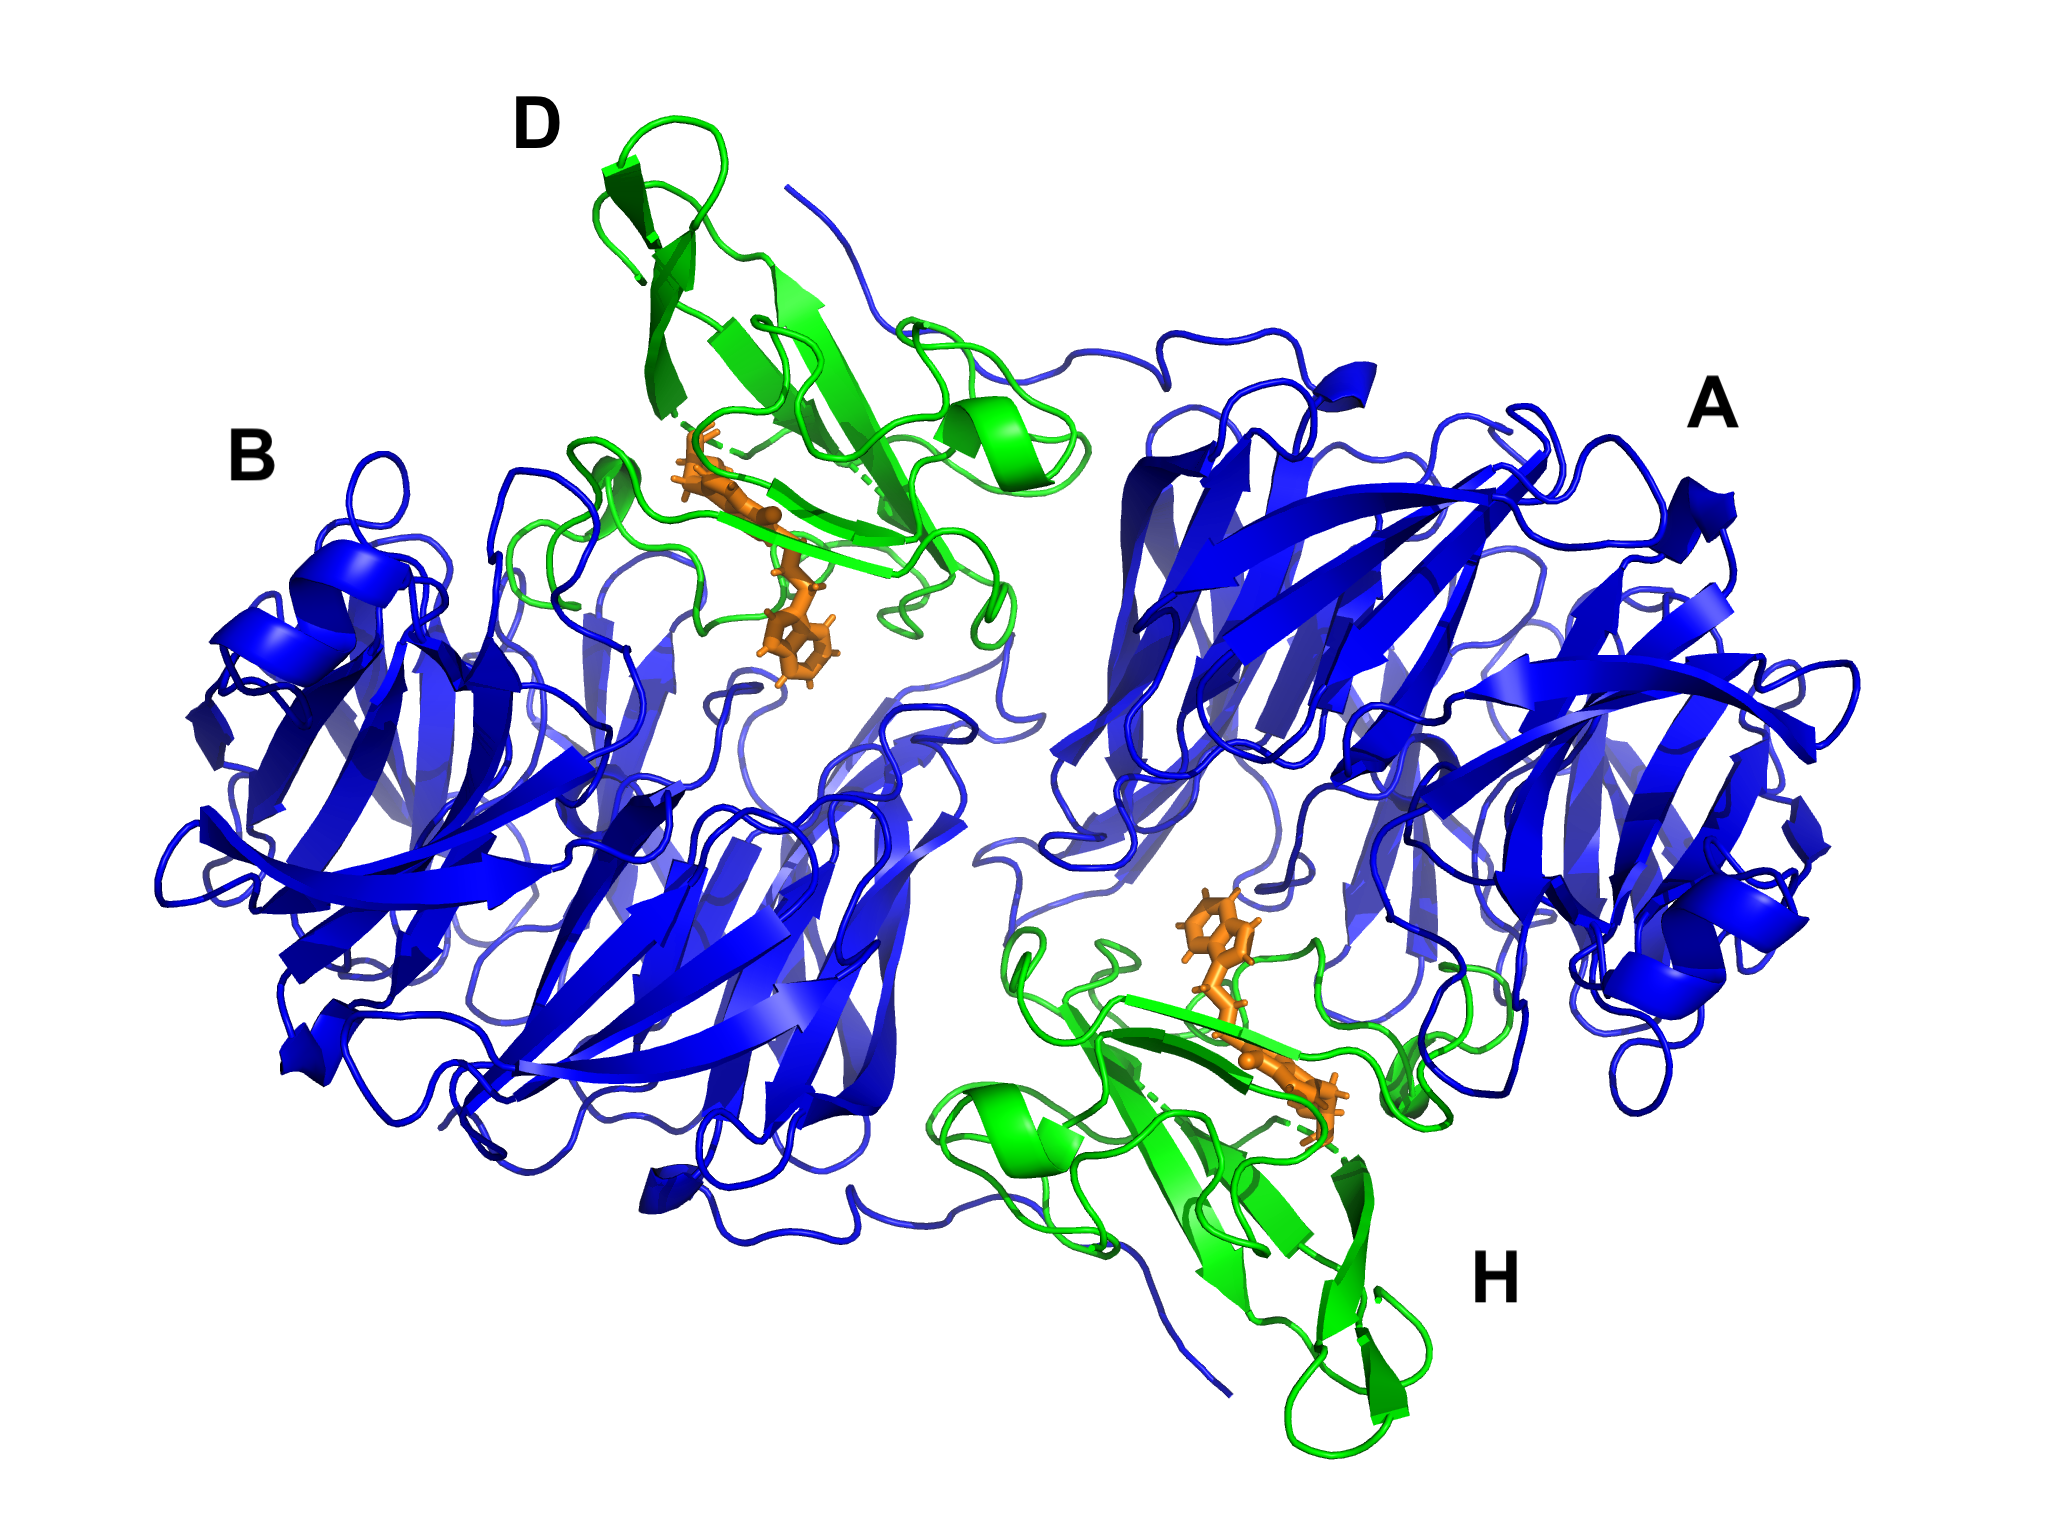
\includegraphics[width=0.8\textwidth]{chapters/aadh/figures/aadh_full_structure.png}
    \label{fig:aadh_full_structure}
\end{figure}

Aromatic amine dehydrogenase (AADH) was isolated from Alcaligenses faecalis \cite{nozakiAromaticAmineDehydrogenase1987} a gram-negative soil bacterium \cite{govindarajAromaticAmineDehydrogenase1994a}. Amines are natural by products of human activity and their degradation is an is an important part of the natural cycle which maintains their balance within organisms and the environment \cite{chistoserdovCloningSequencingMutagenesis2001}. AADH and the other known amine dehydrogenase, methylamine dehydrogenase (MADH) are of continued scientific interest because of their large kinetic isotope effect (KIE) \cite{hyunUnusuallyLargeIsotope1995a}\cite{basranImportanceBarrierShape2001a}\cite{basranEnzymaticHTransferRequires1999}  and the potential role of enzyme dynamics in their function \cite{mcgeaghProteinDynamicsEnzyme2011}\cite{glowackiProteinDynamicsEnzyme2012a}\cite{glowackiTakingOckhamRazor2012b}. Both MADH and AADH contain the tryptophan tryptophylquinone (TTQ) prosthetic group \cite{govindarajAromaticAmineDehydrogenase1994a}\cite{McIntire817}, formed from two cross linked tryptophyl residues. AADH has an $\alpha_{2}\beta_{2}$ structure shown in figure \ref{fig:aadh_full_structure}. The larger $\alpha$ chains have a mass of $\simeq \SI{39}{\kilo\dalton}$ (shown in green and labelled A \& B in the crystal structure) while the smaller $\beta$ chains (shown in red, labelled D and H in the crystal structure) have a mass of $\simeq \SI{18}{\kilo\dalton}$. The D and H chains contain the TTQ prosthetic group that forms part of the active site (shown as purple spheres, after reaction with tryptamine). 


\begin{figure}[p]
    \centering
    \mycaption{The proposed reaction mechanism of AADH, adapted from figure 2 in \cite{masgrauAtomicDescriptionEnzyme2006}. The TTQ prosthetic group is shown in purple, the Asp128$\beta$ group in red and the tryptamine substrate in blue. The boxed step $4$ is the rate determining tunnelling step and step $7$ is the oxidation step. }
    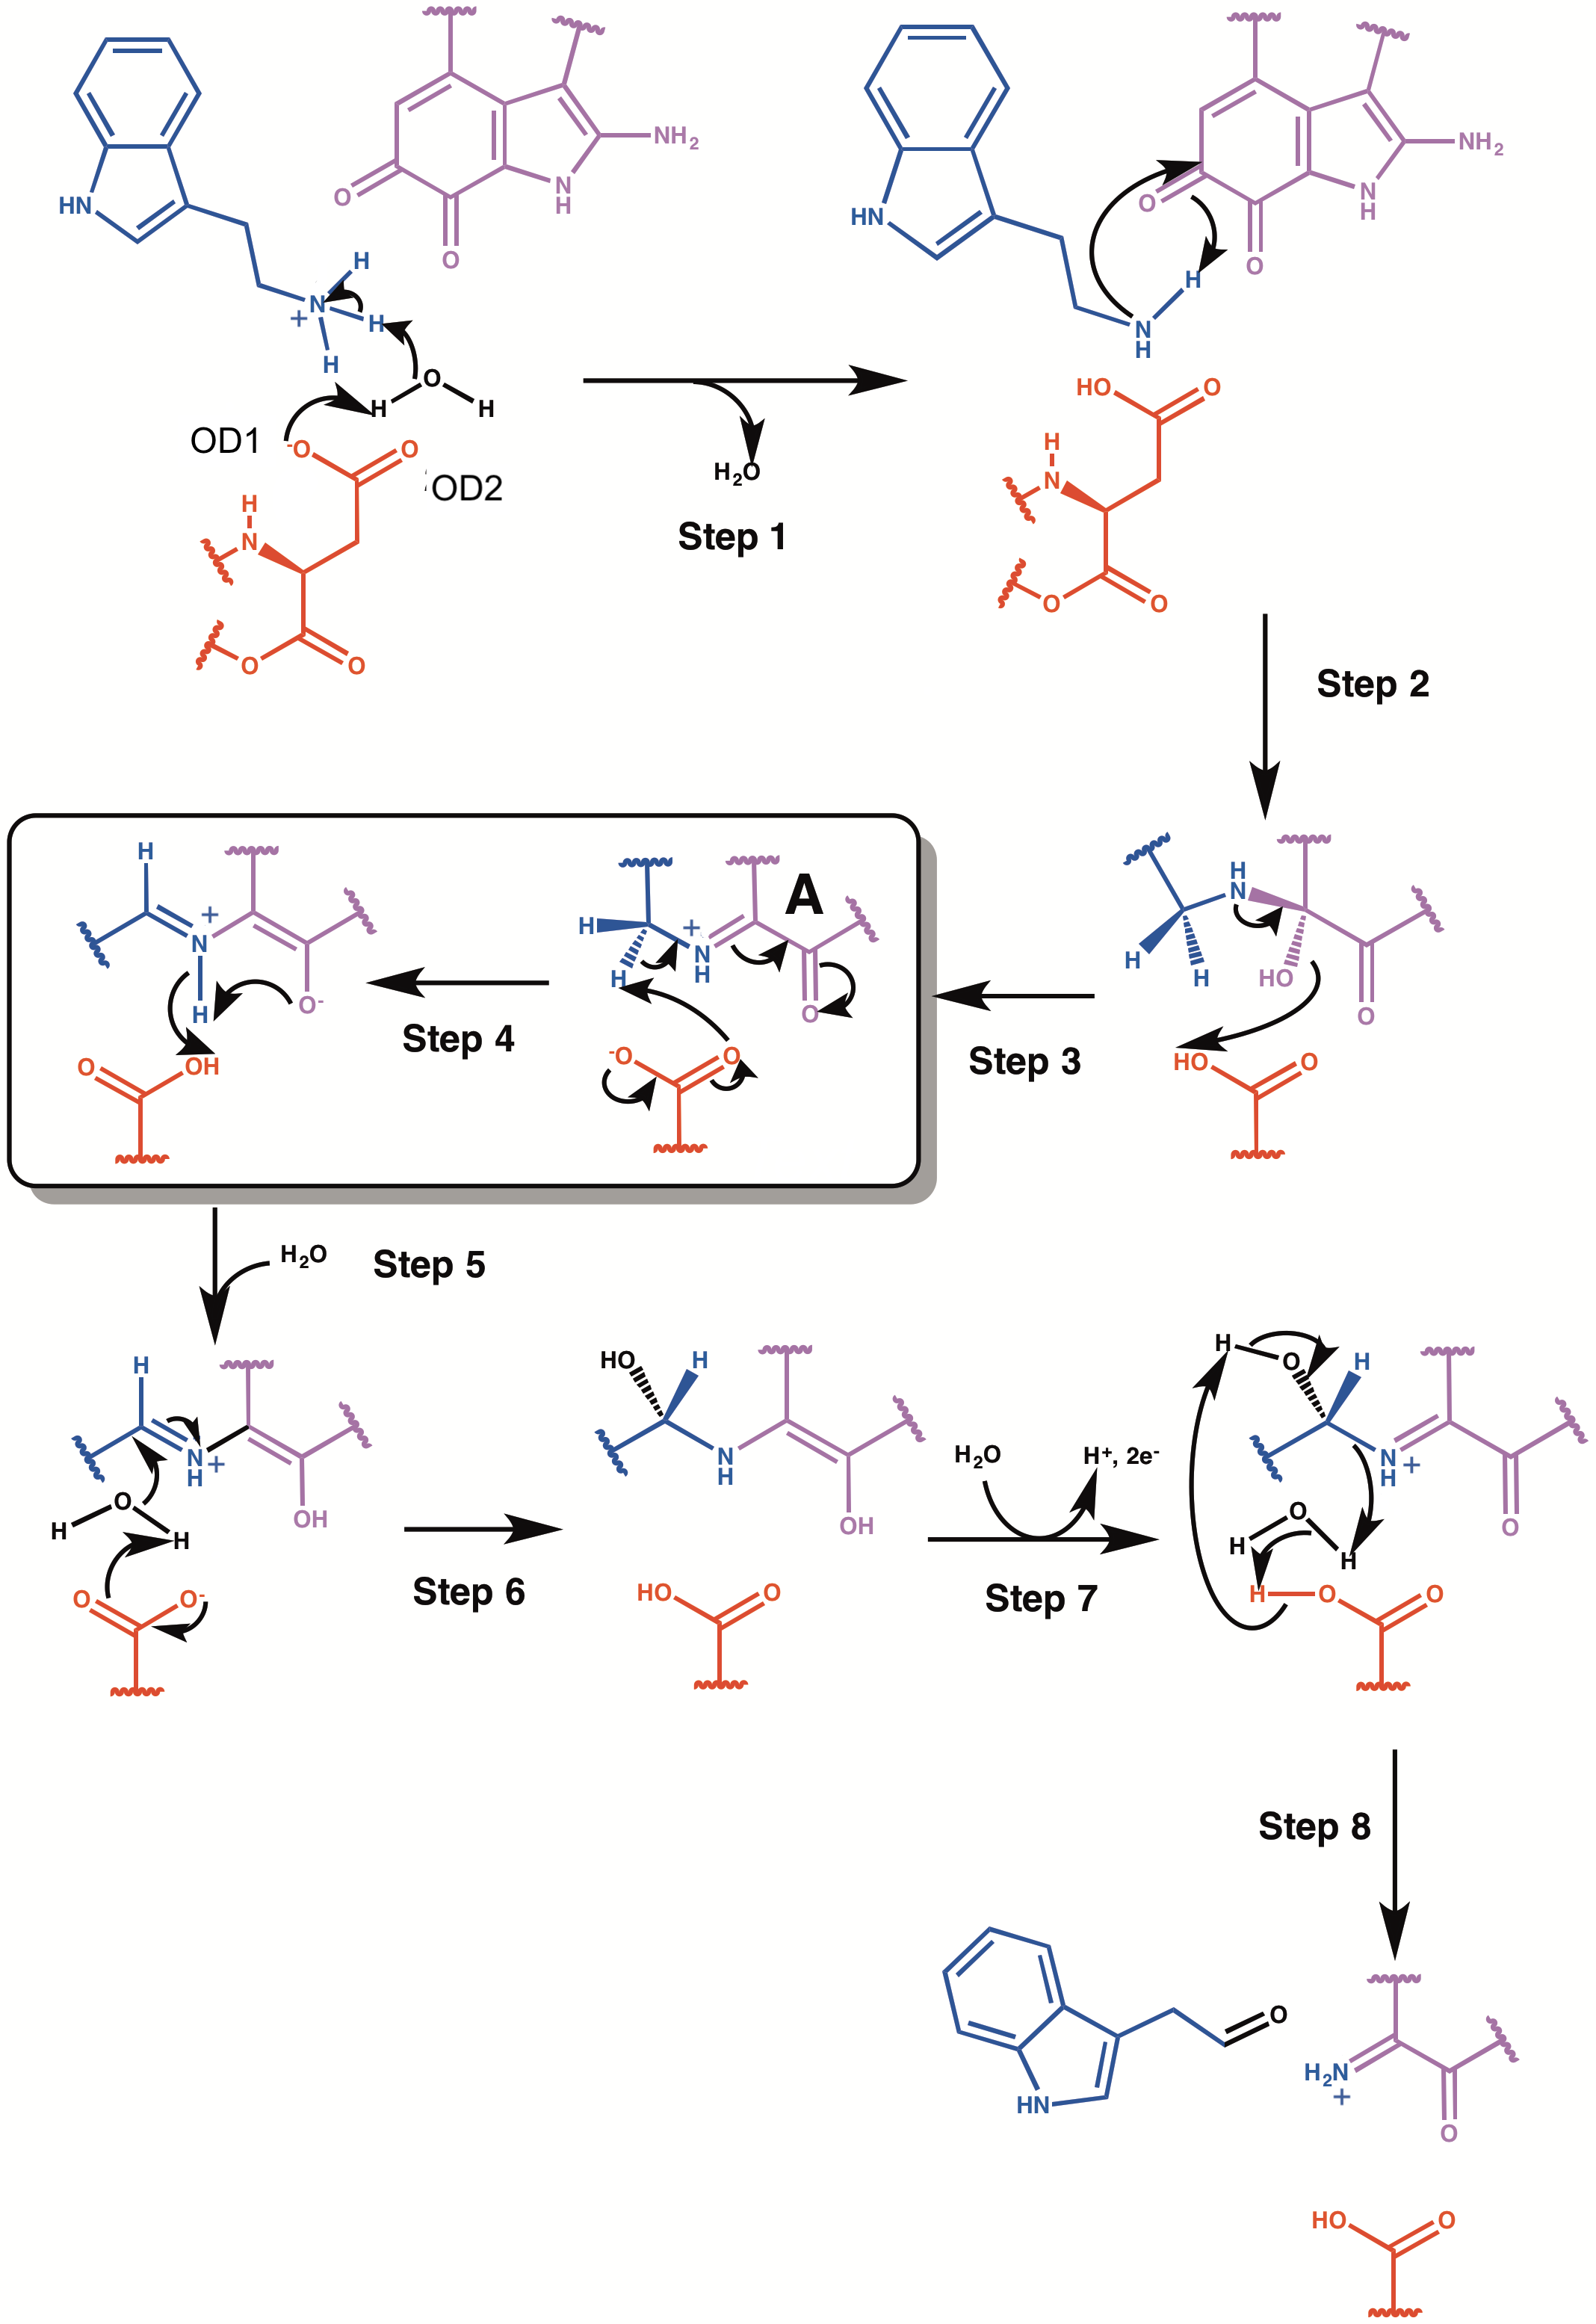
\includegraphics[width=0.8\textwidth]{chapters/aadh/figures/aadh_mechanism.png}
    \label{fig:aadh_mechanism}
\end{figure}

The reaction mechanism of AADH was proposed in \cite{hyunMechanisticStudiesAromatic1995a} and more fully elucidated by a combination x-ray crystallography, experimental and QM/MM (with increasing levels of theory) in \cite{masgrauAtomicDescriptionEnzyme2006}\cite{masgrauTunnelingClassicalPaths2007} and \cite{ranaghanInitioQMMM2017} using tryptamine as a substrate. 
The reaction mechanism is shown in figure \ref{fig:aadh_mechanism}, adapted from figure 2 in \cite{masgrauAtomicDescriptionEnzyme2006}.  The TTQ prosthetic group, attached to the $\beta$ sub-unit, is shown in purple, the protonated tryptamine substrate is shown in blue and the Asp128 residue is shown in red.  The mechanism starts with the enzyme substrate complex of the protonated tryptamine situated next to the TTQ group and Asp128 residue.  The tryptamine is deprotonated by oxygen 1 of the Asp128 residue via a bridging water molecule (step 1).  The nitrogen atom on the tryptamine attacks one of the carbonyl groups of the TTQ residue to form a carbinol-amine intermediate (step 2) that then goes on to form the iminoquinone intermediate labelled `A' (step 3).  Intermediate A was not observed directly but was inferred from the crystal structure of an analogous complex using phenylhydrazine in place of tryptamine.  Step 4, shown boxed, is the rate determining step and involves the tunnelling of a proton from the tryptamine carbon atom adjacent to the nitrogen, to an oxygen atom of the Asp128 residue.  The proton is shown here accepted by oxygen 2 of the Asp128 carboxylate group, but in principle oxygen 1 could also serve as an acceptor. The oxyanion on the TTQ/substrate group (hereafter referred to as TTW) is then neutralized by protonation from Asp128 via the hydrogen atom on the protonated Schiff base (step 5). Water is introduced and in step 6 attacks the Schiff base to form a carbinolamine intermediate that is then oxidized in step 7.  The carbinolamine is then hydrolysed in step 8 and releases the aldehyde.  


The experimental free energy barrier for this reaction is $\simeq \SI{12.7}{\kilo\cal\per\mol}$ at $T=\SI{300}{\kelvin}$ with a primary kinetic isotope effect of $55 \pm 6$, independent of temperature for $T =$ \SIrange{278}{298}{\kelvin}\cite{masgrauAtomicDescriptionEnzyme2006}. The high KIE is indicative of the hydrogen tunneling through the reaction barrier  \cite{masgrauAtomicDescriptionEnzyme2006}\cite{kohenEnzymeCatalysisClassical1998}\cite{antoniouInternalEnzymeMotions2001}\cite{antoniouLargeKineticIsotope1997}\cite{allemannQuantumTunnellingEnzymecatalysed2009}. The rate determining hydrogen abstraction can proceed to either OD1 or OD2 of the Asp128. These two atoms are distinguished by the hydrogen bonded network: OD2 is hydrogen bonded to Trp160, and OD1 to Thr172 as shown in figure \ref{fig:aadh_active_site}. In the previous AADH simulation studies,  \cite{masgrauAtomicDescriptionEnzyme2006}\cite{masgrauTunnelingClassicalPaths2007}\cite{ranaghanInitioQMMM2017}, the authors labelled OD1 as O2 and OD2 as O1, this convention is not adopted here as the accessible conformations allow OD1 and OD2 to bond to both Trp160 and Thr172, the force-field atoms names will be retained. 

The authors of \cite{ranaghanInitioQMMM2017} calculated the potential energy surface for pathways to both oxygen atoms using nudged elastic band with QM/MM using DH\&HLYP/6-311+G(d)/MM. Although not the aim of this study, they incorporated zero-point energy, tunneling and entropic contributions of previous studies \cite{masgrauAtomicDescriptionEnzyme2006}\cite{masgrauTunnelingClassicalPaths2007} to estimate the free energy barriers to O2 and O1 as $\SI{11.5}{\kilo\cal\per\mol}$ and $\SI{8.84}{\kilo\cal\per\mol}$ respectively, meaning both pathways are distinct but indistinguishable from the experimental free energy.  

The role of protein dynamics in promoting tunneling has proved controversial in part due to the problems with identifying the contribution of the enzyme over a suitable reference reaction [][][]. However, current theory \cite{kuznetsovProtonHydrogenAtom1999a}\cite{masgrau2004hydrogen} uses two types of protein dynamics to explain the rate constants and the temperature dependence of the KIE. `Active dynamics' which enhance the probability of tunneling occurring in a given conformation, and `passive dynamics' which re-arrange the enzyme to achieve such a suitable conformation. Active vibrations, on the sub-picosecond timescale,  have been identified in AADH \cite{johannissenEnzymeAromaticAmine2008}\cite{johannissenProtonTunnelingAromatic2007} which act to promote the tunneling reaction.  However, the KIE in AADH is independent of temperature \cite{masgrauAtomicDescriptionEnzyme2006}, indicative of passive dynamics being the dominant factor in explaining the observed rate constant. Furthermore in  \cite{glowackiProteinDynamicsEnzyme2012a}\cite{glowackiTakingOckhamRazor2012b} the authors showed that the kinetics and KIEs of a number of enzymes with large KIEs, including AADH, could be fitted to a simple extension of Transition State Theory (TST). This model posits two inter-converting enzyme conformations each linked to a reaction coordinate with different reaction barriers. While this model can be made to  realistically fit experimental data, the conformers, their number and the exact values of the model parameters have not been fully validated. 

It is clear that an accurate and comprehensive description of the conformational dynamics of AADH would be useful in adding to the ongoing debate of enzyme dynamics and their role in catalysis. This chapter describes the first step towards this goal, the creation of molecular dynamics data set and the estimation of important parameters of the system for use in later chapters. The structure is as follows: section \ref{sec:aadh_md} describes the creation of a molecular dynamics data set; section \ref{sec:aadh_validation} validates the data set, in particular active sites and compares to previous work; section \ref{sec:aadh_msm} describes the creation of a Markov State Model in order to estimate the Markov lag time and the number of dominant eigenvalues which will be used in the optimisation of MSM hyper-parameters in chapters \ref{chap:msm} and \ref{chap:hmm}. 

\section{Molecular dynamics}\label{sec:aadh_md}

The starting point was crystal structure of AADH in Schiff base form after reaction with tryptamine, PDB accession code 2AGY \cite{masgrauAtomicDescriptionEnzyme2006}. Dr Kara Ranaghan prepared the PDB file by adding the missing hydrogen atoms, determining the protonation states of titratable residues, created the disulphide bridges and parameterized the TTQ/Tryptamine Schiff base (structure A in figure \ref{fig:aadh_mechanism}, custom residue name TTW) for use with the CHARMM-22 forcefield \cite{a.d.mackerellAllAtomEmpiricalPotential1998} as part of the computational part of \cite{masgrauAtomicDescriptionEnzyme2006}, \cite{masgrauTunnelingClassicalPaths2007} and \cite{ranaghanInitioQMMM2017}.  The first 23 residues of the D and H chains, which were unobserved in the crystal structure, were not modelled. This concludes Dr Ranaghan's contribution to this work. 

The atom types in TTW were changed to be compatible with the CHARMM-36 \cite{huangCHARMM36AllatomAdditive2013} force-field although the TTW parameters remained the same. The CHARMM package, version 42a2 \cite{brooksCHARMMBiomolecularSimulation2009} was used to create a protein structure file (PSF). 

A solvation shell tracking the surface of the protein was created using the package Solvate version 1.0 \cite{grubmullerSolvate} which I modified to take into account the CHARMM extended PSF format. The shell was $\SI{12.0}{\angstrom}$ thick, the maximum boundary curvature radius of the solvent surface was $\SI{100}{\angstrom}$, and $10$ Gaussian functions were used to determine the solvent surface. This structure was further solvated to create a cubic simulation cell of size $\SI{130}{\angstrom}$ using the package Visual Molecular Dynamics (VMD) version 1.9.3 \cite{HUMP96} with a boundary parameter equal to $\SI{1.2}{\angstrom}$. The size of the box was chosen so that the minimum distance between the enzyme and the edge of the simulation cell was  $\SI{14}{\angstrom}$. The system was neutralized with VMD using sodium chloride to attain a concentration of $\SI{0.15}{\molar}$. 
The minimization, heating and equilibration steps were performed in CHARMM with the OpenMM \cite{OpenMMRapidDevelopment} plug-in using the CHARMM-36m \cite{huangCHARMM36AllatomAdditive2013} force-field. The electronic non-bonded forces in all steps were treated with partial mesh Ewald summation with a cut-off of $\SI{14}{\angstrom}$, all other parameters were set to their default values. The SHAKE \cite{ryckaertNumericalIntegrationCartesian1977b} algorithm was used throughout to constrain the hydrogen atoms. The minimization proceeded by first constraining all heavy atoms  using a Root Mean Square Deviation (RMSD) constraint with a mass weighted force constant of $\SI{5}{\kilo\cal\per\mol\per\angstrom}$ and then minimizing with $100$ step using the steepest descent algorithm and $3000$ steps of Adopted Basis Newton-Raphson (ABNR) minimization. This was repeated and sequentially limiting the  constraint to the heavy protein atoms, heavy protein backbone atoms, and finally with no constraints. The final unconstrained minimization proceeded with $5000$ instead of $3000$ ABNR minimization. 

The system was heated from $\SI{10}{\kelvin}$ to $\SI{310}{\kelvin}$ in steps of $\SI{25}{\kelvin}$ with a harmonic constraint on the heavy protein backbone atoms with mass weighted force constant of $\SI{5}{\kilo\cal\per\mol\per\angstrom}$ and . At each heating step $\SI{10}{\pico\second}$ of Langevin dynamics in a constant volume, constant temperature ensemble were run with a time-step of $\SI{2}{\femto\second}$ and collision frequency of $\gamma=\SI{5}{\per\pico\second}$. 

The system underwent equilibration in two stages: restrained equilibration and unrestrained equilibration. In the restrained equilibration stage $11 \times \SI{20}{\pico\second}$ iterations of Langevin dynamics were run in an constant pressure, constant temperature ensemble ($P=\SI{1}{\atm}$, $T=\SI{310}{\kelvin}$), with a Langevin collision frequency $\gamma=\SI{1}{\per\pico\second}$, a Monte Carlo barostat with volume moves performed every  $\SI{50}{\femto\second}$, and a time-step of $\SI{2}{\femto\second}$. On the first iteration the backbone atoms had a harmonic constraint with a mass weighted force constant of  $\SI{10}{\kilo\cal\per\mol\per\angstrom}$. On each subsequent iteration the force constant was reduced by $\SI{1}{\kilo\cal\per\mol\per\angstrom}$ until the last iteration had no harmonic constraint. The unconstrained equilibration consisted of $\SI{200}{\pico\second}$ of equilibration was run under the same conditions as before with no constraints. 

The simulation system was transferred from CHARMM to AMBER 16 \cite{caseAMBER} to make use of the improved user interface and post-simulation analysis tools. A single  $\SI{100}{\nano\second}$ trajectory was produced in a constant volume, constant temperature ($T=\SI{310}{\kelvin}$) ensemble, using Langevin dynamics with a collision frequency of $\gamma=\SI{5}{\per\pico\second}$, and a time step of $\SI{2}{\femto\second}$. The non-bonded cut-off distance was reduced to $\SI{12}{\angstrom}$ and SHAKE was used to constrain the hydrogen atoms. Coordinates and velocities were written to disk every $\SI{100}{\pico\second}$.  

The coordinates and velocities at every \SIlist[list-final-separator = { ... }]{1; 2; 100}{\nano\second} were used to seed $100 \times \SI{100}{\nano\second}$ new trajectories, run under the same conditions. These $100$ trajectories constituted the AADH data set. 

\section{Validation}\label{sec:aadh_validation}

An error was found in the preparation of the initial structure \emph{after} completion of the simulations. The disulphide bridge between Cys81 and Cys113 on the H chain (but not on the D chain) had not been created, instead the two thiol groups were left unoxidized. This will be discussed in full below. 

\begin{figure}
    \centering
    \mycaption{Structural similarity of trajectory used to seed the the final production trajectories. Panel (a) shows the $\alpha$-Carbon RMSD relative to the crystal structure, (b) shows the distribution of all pairwise $\alpha$-Carbon RMSD.   }
    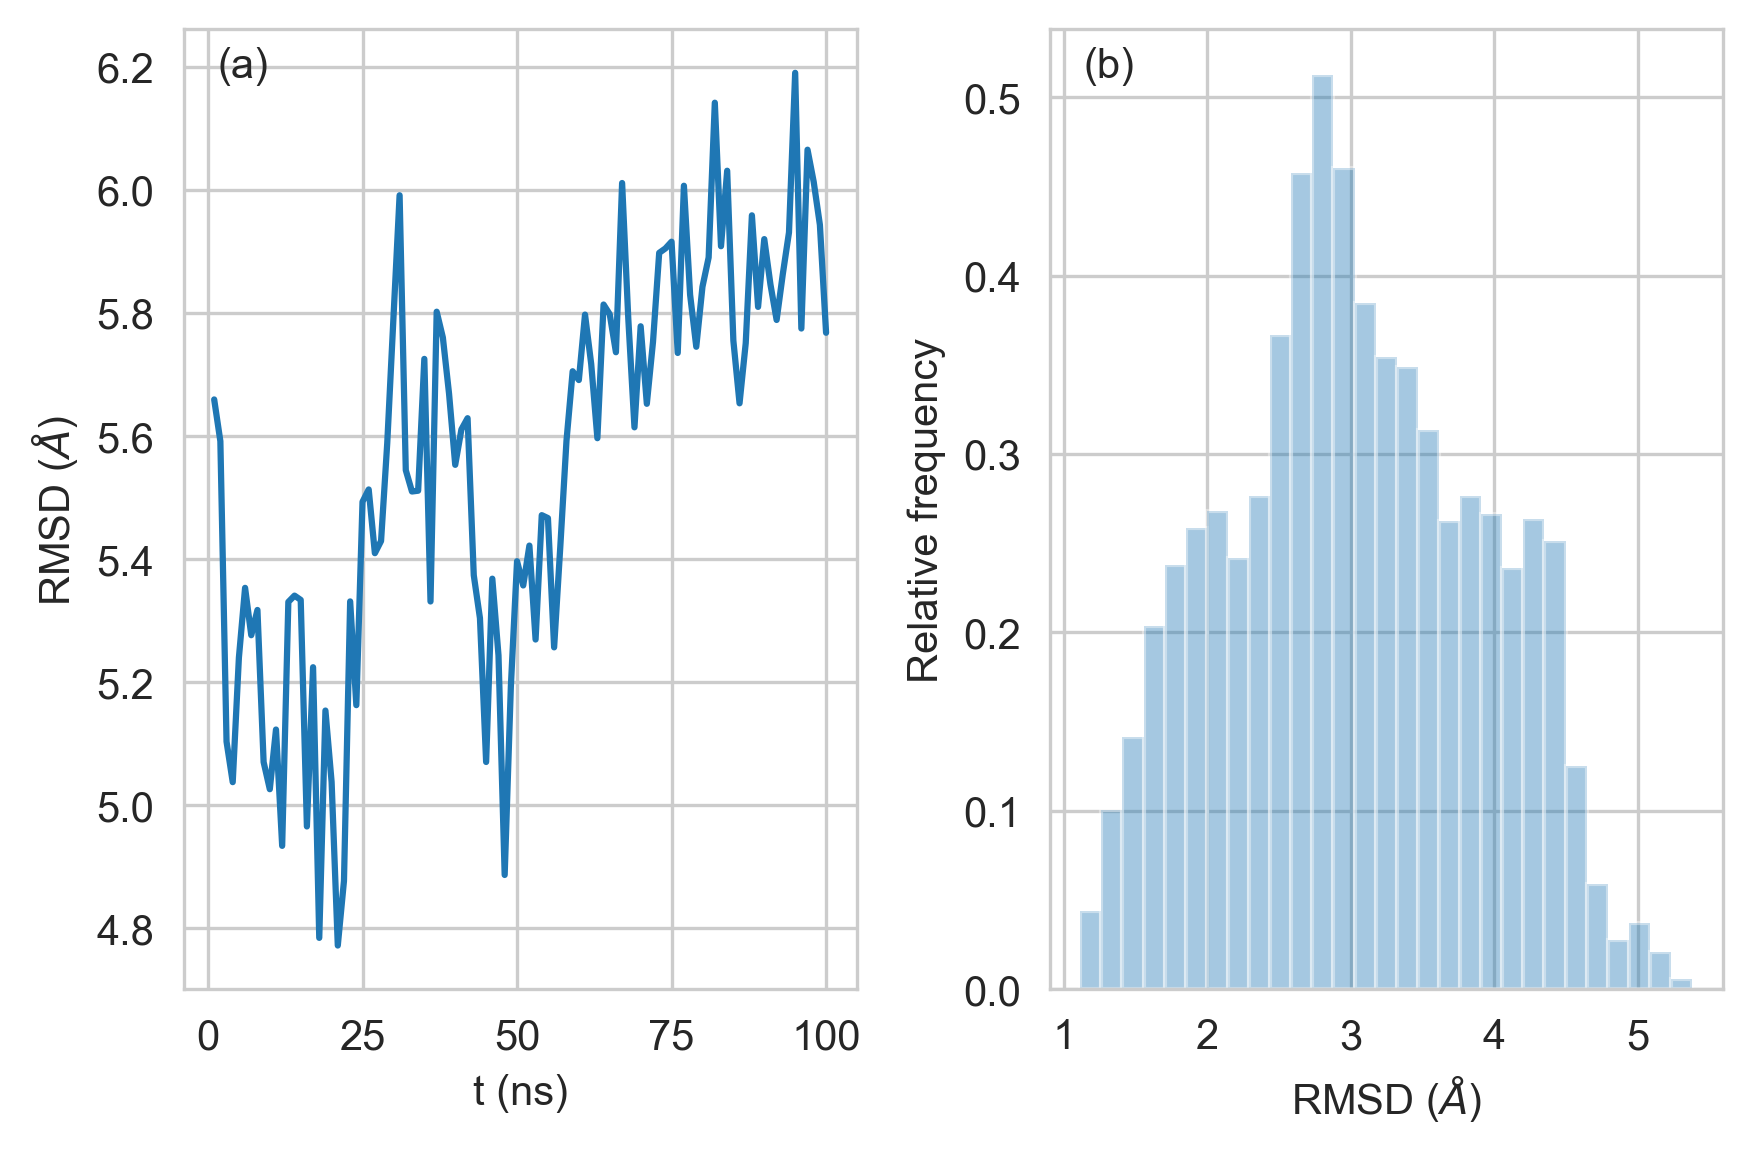
\includegraphics[width=0.8\textwidth]{chapters/aadh/figures/rmsd_seed_trajectory.png}
    \label{fig:rmsd_seed_traj}
\end{figure}

 The structural similarity between the initial frame of the each of the $100$ production trajectories is shown in figure \ref{fig:rmsd_seed_traj}. Panel (a) shows the $\alpha$-Carbon RMSD, relative to the crystal structure, which clearly shows serial correlation between initial frames, especially for those at $t>\SI{60}{\nano\second}$. Panel (b) shows the distribution of $\alpha$-Carbon RMSD values between each pair of initial frames (so there are $\sfrac{1}{2}\cdot 100\cdot 99 = 4950$ values) which demonstrate a range of differences between the initial conformations. $\SI{50}{\percent}$ of the initial structures have an RMSD of $\SI{3.0}{\angstrom}$ or larger.  

Each trajectory was checked for structural stability over the course of the simulations by calculating the RMSD of the $\alpha$-Carbons atoms relative to the crystal structure, shown in figure \ref{fig:rmsd_ca}. The majority of the trajectories showed no breakdown in structure, with  \SI{95}{\percent} of the frames within \SIrange{4.5}{6.4}{\angstrom} of the crystal structure. However, seven of the trajectories ($24, 27, 30, 42, 78, 87$ and $97$) had an RMSD trajectory which increased over time, leaving the upper \SI{95}{\percent} bound by at least the final frame, shown in figure \ref{fig:rmsd_ca}. To check that these trajectories weren't losing their secondary structure the number of residues in each simplified secondary structure class \cite{kabschDictionaryProteinSecondary1983} over time was calculated. Each trajectory showed a stable number of residues in each class as shown in figure \ref{fig:dssp_trajs}.

\begin{figure}
    \centering
    \mycaption{The crystal structure of the active site of AADH. This definition is taken from \cite{ranaghanInitioQMMM2017}. The yellow dashed lines show the important stabilizing hydrogen bonds as well as the H/O distances involved in the rate determining step.  The reactive hydrogen atoms are labelled HI-2 and HI-3. The acceptor oxygen atoms are labelled OD2 and OD1 which correspond to O1 and O2 in \cite{masgrauAtomicDescriptionEnzyme2006} respectively. All other hydrogen atoms are hidden. Backbone carbonyl bonds may appear as single bonds due to the camera angle.}
    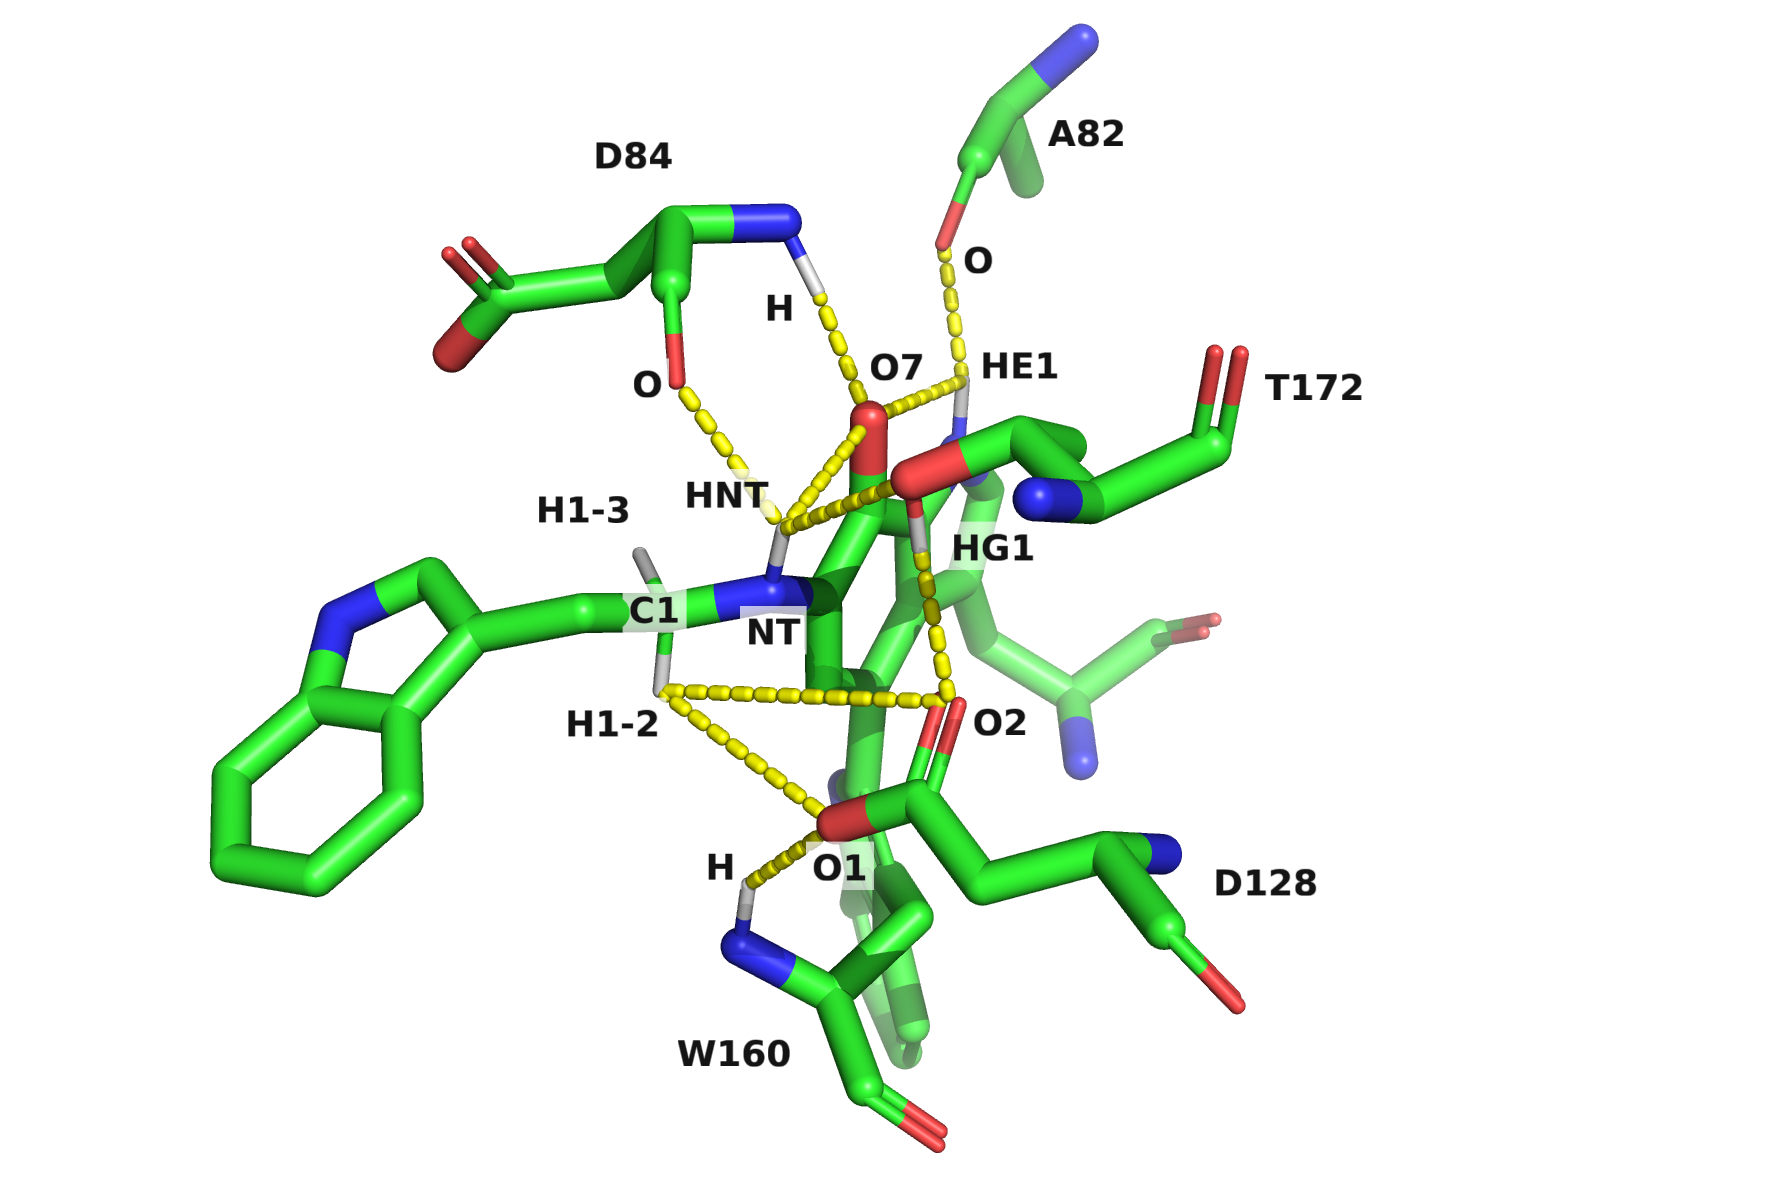
\includegraphics[width=0.8\textwidth]{chapters/aadh/figures/aadh_active_site.png}
    \label{fig:aadh_active_site}
\end{figure}

\begin{figure}
    \centering
    \mycaption{The distribution of heavy atom RMSD, relative to the crystal structure of the active sites in chain D (blue) and H (orange). }
    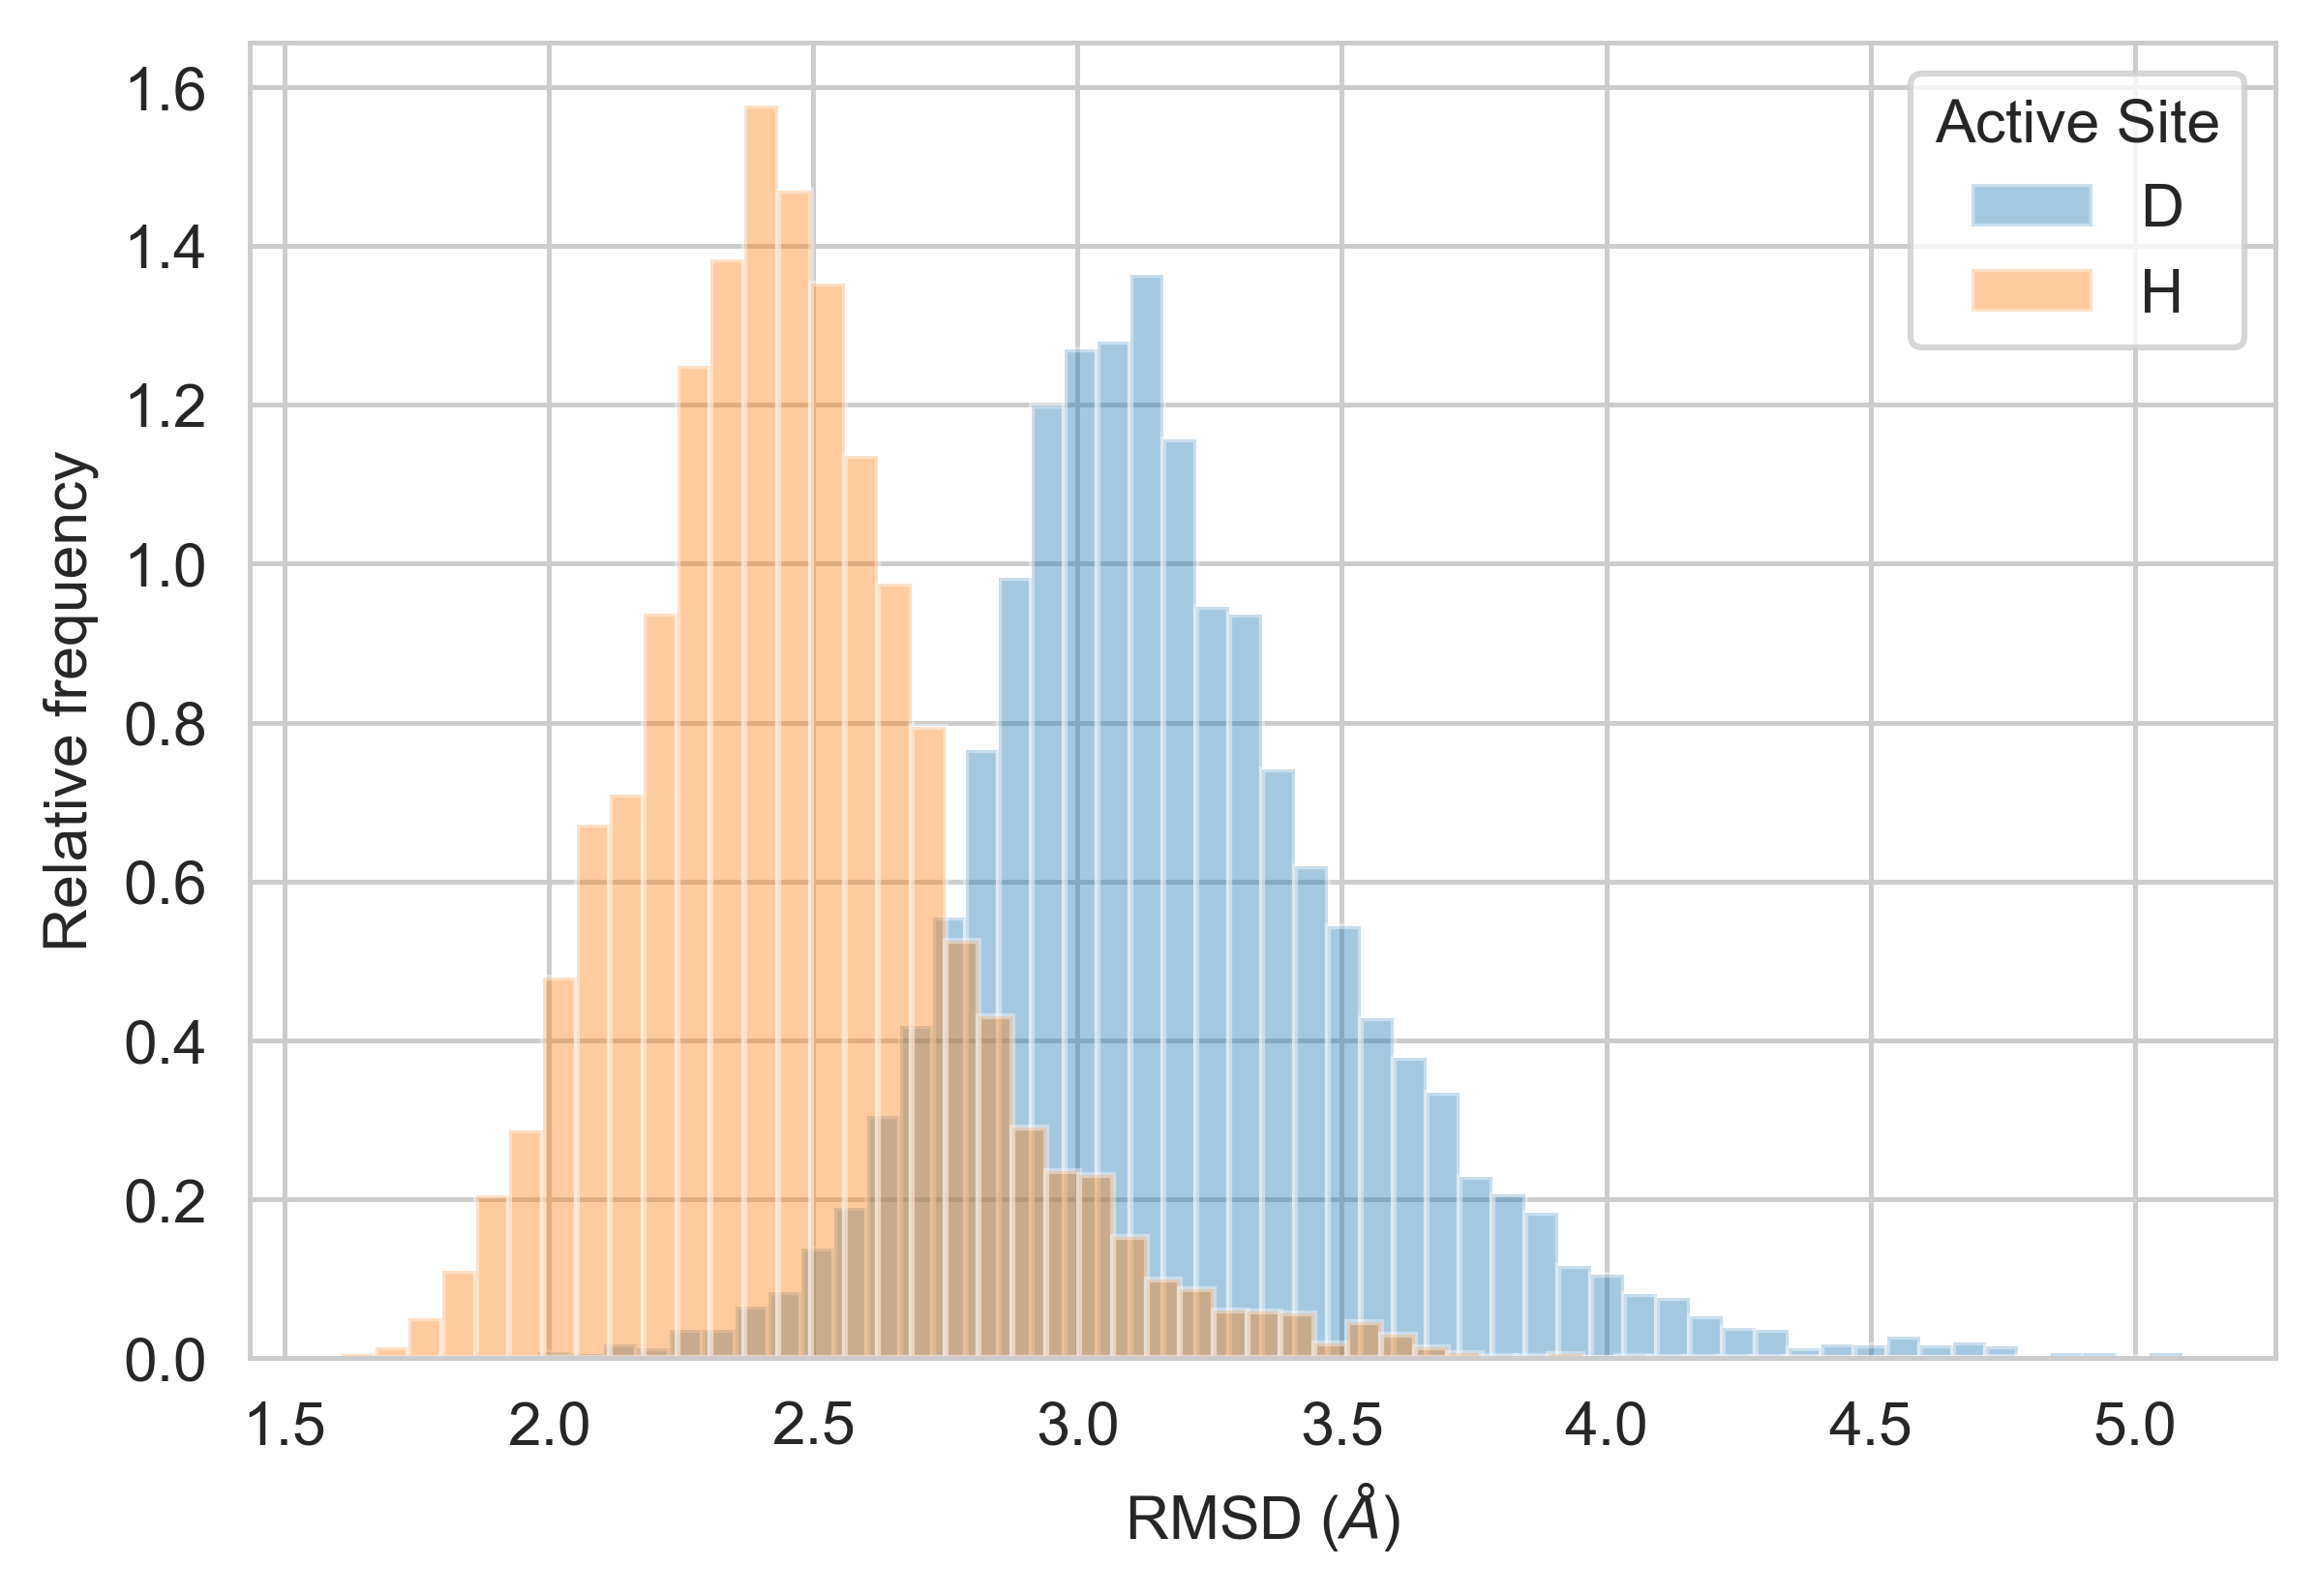
\includegraphics{chapters/aadh/figures/rmsd_dististribution.png}
    \label{fig:as_rmsd_dist}
\end{figure}

The active site of the enzyme was defined (following \cite{ranaghanInitioQMMM2017}, \cite{masgrauAtomicDescriptionEnzyme2006} and \cite{masgrauTunnelingClassicalPaths2007}) as the following residues in both chains D and H: Ala82, Asp84, TTW109, Asp128, Trp160 and Thr172. The TTW residue is the TTQ prosthetic group after reaction with the tryptamine substrate to form the Schiff base intermediate. Any references to TTQ will refer to the potion of TTW coming from TTQ originally and not the unreacted prosthetic group. The crystal structure of the active site is shown in figure \ref{fig:aadh_active_site}. 

The structures of the two active sites were compared to the crystal structure. The distribution of the heavy atom RMSD, relative to the crystal structure, is shown in figure \ref{fig:as_rmsd_dist}. This shows that, surprisingly, the H active site, without the di-sulphide bridge is more structurally similar to the crystal structure than the D active site. 

\begin{figure}
    \centering
    \mycaption{Distribution of bond distances in the active site. Panels (a) - (d) show the four combinations of acceptor ion (O1, O2) - proton (H1-2, H1-3) distances; panels (e) and (f) are the two donor (C1) acceptor (O1, O2) distances; the remaining panels are the hydrogen bonds in the active site.}
    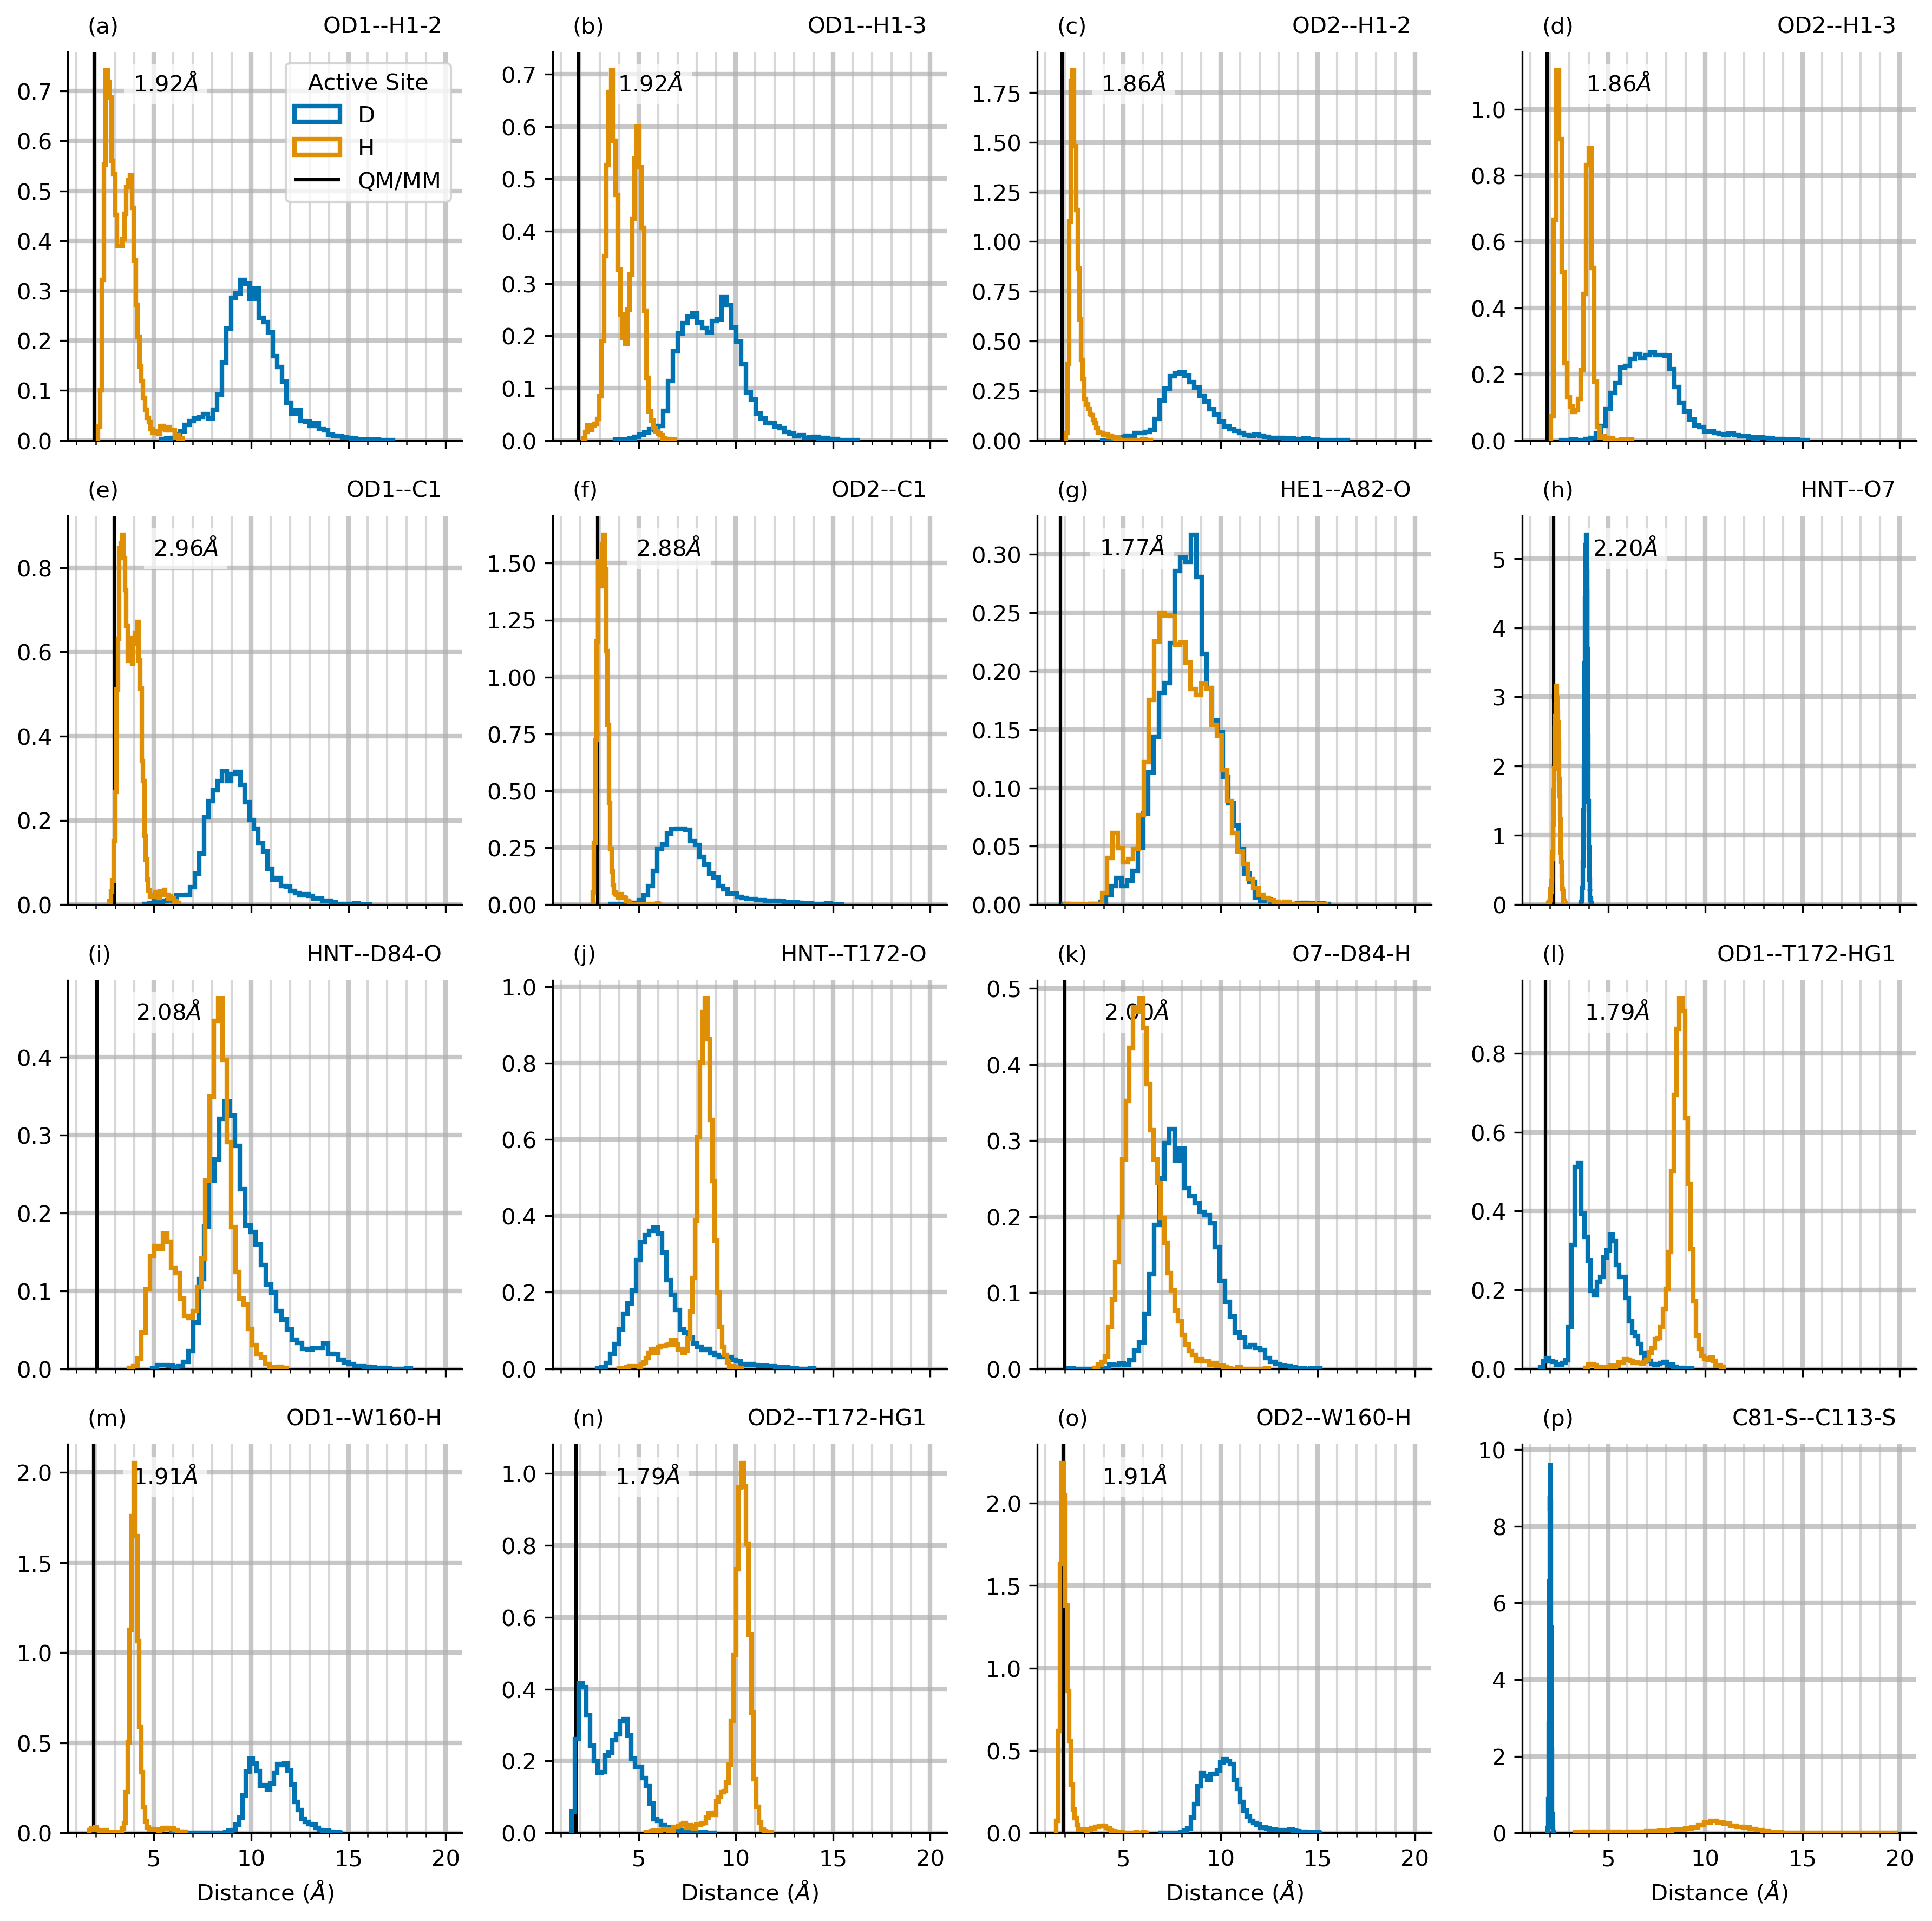
\includegraphics[width=0.8\textwidth]{chapters/aadh/figures/bond_distances_dist.png}
    \label{fig:bond_dist}
\end{figure}

To understand this difference between the active sites further and to explore the similarities between these simulations and the most accurate previous work in \cite{ranaghanInitioQMMM2017}, the distribution of important interatomic distances were calculated and compared. Figure \ref{fig:bond_dist} shows these bond distributions in blue for the D active site and in orange for the H active site. The black vertical lines with labels are the QM/MM interatomic distances in the reactant state\footnote{An average over the pathways to OD1 and OD2 are taken where appropriate.}, taken from table 3 of \cite{ranaghanInitioQMMM2017}. Where possible I have kept the atom labels the same as \cite{ranaghanInitioQMMM2017}, the exceptions are the atoms directly involved in bond breaking and formation. The correspondence between the interatomic distances in \cite{ranaghanInitioQMMM2017} and figure \ref{fig:bond_dist}, and their description are as follows: 
\begin{enumerate}
    \item OD1/OD2---H1:  The bond being formed. These correspond to all four combinations of distances between OD2/OD1 (respectively) and H1-2, H1-3. Shown in panels (a) through (d). 
    \item OD1/OD2---C1: The donor/acceptor distance. These are the two combinations of distances between OD2/OD1 (respectively) and C1. Shown in panels (e) and (f). 
    \item HE1---A82-O: Inter-residue hydrogen bond between HE1 of the TTQ prosthetic group and the Ala82 backbone oxygen atom, shown in panel (g). 
    \item HNT---O7: Intra-residue hydrogen bond in the TTW residue. Shown in panel (h). 
    \item HNT---D84-O: Inter-residue hydrogen bond between the TTW residue and the backbone oxygen atom of the Asp84 residue. 
    \item HNT---T172-O: This is not described in \cite{ranaghanInitioQMMM2017} but is included because of its potential to form a hydrogen bond in certain conformations. Shown in panel (j). 
    \item O7---D84-H: Inter-residue hydrogen bond between the TTW residue and the backbone amide hydrogen atom of the Asp84 residue. Shown in panel (k). 
    \item OD1---T172-HG1/W160-H: The inter-residue hydrogen bond between the acceptor oxygen atom OD1 of D128 and hydrogen atoms on the Thr172 and Trp160 residues respectively. Shown in panels (l) and (m).
    \item OD2---T172-HG1/W160-H: The inter-residue hydrogen bond between the acceptor oxygen atom OD2 of D128 and hydrogen atoms on the Thr172 and Trp160 residues respectively. Shown in panels (n) and (o).\label{o1_t172}
    \item C81-S---C113-S: The di-sulphide bond in the D and H chains. Shown in panel (p). \label{cs_cs} 
\end{enumerate}

The missing di-sulphide bond has clearly had a large effect on H active site.  The distribution of the S---S distances in the H active site, shown in panel (p) varies between  \SIrange{3}{20}{\angstrom} compared to the effectively fixed distance of $\simeq \SI{2}{\angstrom}$ in the D active site. The distributions in the D active site show greater variance and do not, in general, overlap with those in the H active site.

The O---H distances are smaller, closer to the QM/MM values, and show less variation in the H active site compared to the D active site by a significant margin (panels (a) - (d)). The distances in the H site are almost all less than \SI{5}{\angstrom} (within $\simeq\SI{3}{\angstrom}$ of the QM/MM values), where almost all the D active site values are between \SIrange{5}{10}{\angstrom}. The donor/acceptor distances, C---O (panels (e) and (f)) show a similar story. The closest hydrogen atom to both acceptor oxygen anions in the H active site is H1-2, the differences in the D active site are less obvious. These differences are due to the crystal structure preparation and missing di-sulphide bond as: (1) there is no difference between the active sites in the crystal structure (the difference in heavy atom RMSD is $\SI{0.00}{\angstrom}$); and (2) the broken di-sulphide bond is incompatible with the pathways determined in \cite{masgrauTunnelingClassicalPaths2007}
and \cite{ranaghanInitioQMMM2017}. 

There is no conclusive similarity between the QM/MM results and these simulations with respect to the stabilization of OD1 and OD2 by Thr172 and Trp160 by hydrogen bonds. This is important as it is these hydrogen bonds which help define the difference in between the hydrogen abstraction pathways. The orientation of Trp160-H, OD2, OD1 and Thr172-HG1 in the crystal structure and QM/MM is approximately linear. For OD1 to be hydrogen bonded with Thr172, the bond lengths would be ordered OD1---Thr172-HG1 $<$ OD1-Trp160-H, i.e. panel (l) $<$ panel (m). While for OD2 to be hydrogen bonded with Trp160, the bond lengths would be ordered OD2---Thr172-HG1 $>$ OD2-Trp160-H, i.e. panel (n) $>$ panel (o). This is clearly the case for the H active site. In the D active site, Asp128 has moved away from Trp160 entirely as seen by comparing the distributions in  panels (m) and (o)  with panels (l) and (n). Noting that TTW is covalently bonded to Trp160, this is then consistent with the picture in panels (a) through (f) where OD1 and OD2 are between \SIrange{5}{15}{\angstrom} from the relevant atoms on TTW.  

The TTW intra-residue hydrogen bond, HNT---O7, shows good agreement with the QM/MM value in the H active site, while in the D active site it is larger by almost \SI{2}{\angstrom}. The two distinct HNT---O7 bond lengths define whether the NT---C1 bond is either syn or anti the C---O7 carbonyl bond in the tryptophan ring system of TTQ. The anti conformation, with has the shorter HNT---O7 distance, is adopted in active site H and in the crystal structure as shown in figure \ref{fig:aadh_active_site}.  Here the NT---HNT bond points in the same direction as the C---O7 bond and forcing the NT---C1 bond into the anti-conformation. The syn conformation has the has the NT---HNT bond pointing in the opposite direction, forcing the NT---C1 bond to eclipse the the C---O7 carbonyl bond. 

The syn and anti conformations allow radically different conformational states to be accessed as demonstrated in figure \ref{fig:ttw_wiggle}. Each panel shows $500$ conformational states, selected evenly across all trajectories, for the D (panel (a)) and H (panel (b)) active site. The entire TTW residue and carbonyl group of Asp128 is shown and the conformations have been aligned to the tryptophan part of the TTW residue. The only two hydrogen atoms shown are H1-2 \& H1-3 and are coloured white. The syn conformation of the D active site clearly demonstrates a `looser' set of conformations with the  C1-H1 bond pointing away from the acceptor Asp128 residue. The anti conformation of the H active site shows a `tighter' set of conformations with the C1-H1 bond pointing towards the Asp128 residue. 


\begin{figure}
    \centering
    \mycaption{Conformations of the TTW residue in the D and H active sites. Five conformations were taken from each trajectory at intervals of $\SI{20}{\nano\second}$ and aligned along the heavy atoms of the trypotophan part of the TTW residue.  The hydrogen atom shown is the donor atom, all other hydrogen atoms are hidden.}
    \subbottom[Active site D]{
    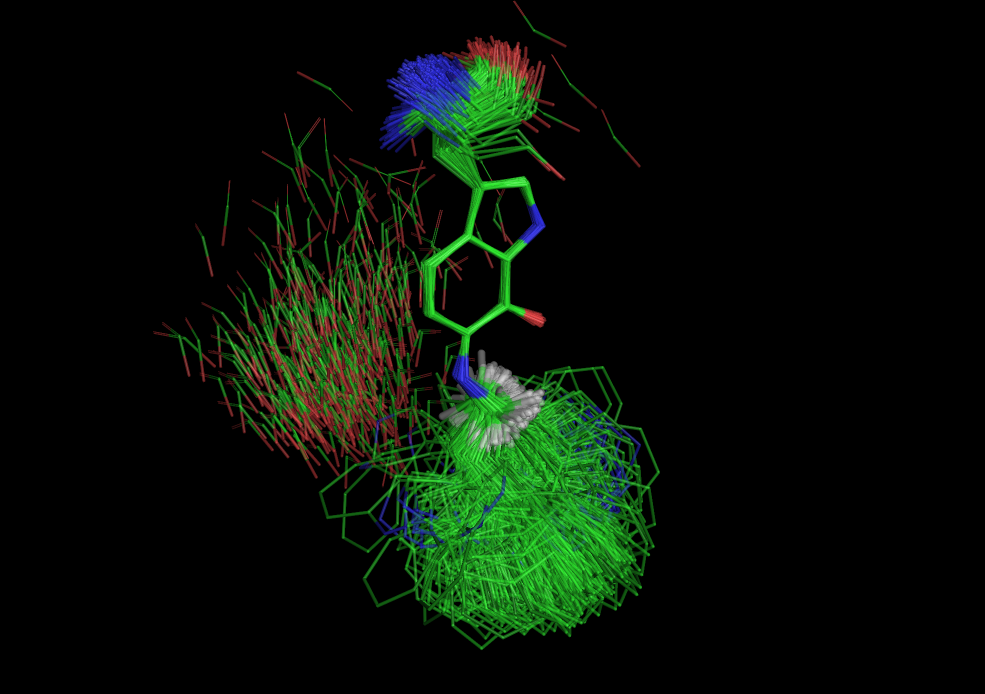
\includegraphics[trim={1cm, 0, 1cm, 0}, clip=True]{chapters/aadh/figures/as_d_wiggle.png}}
    \subbottom[Active site H]{
    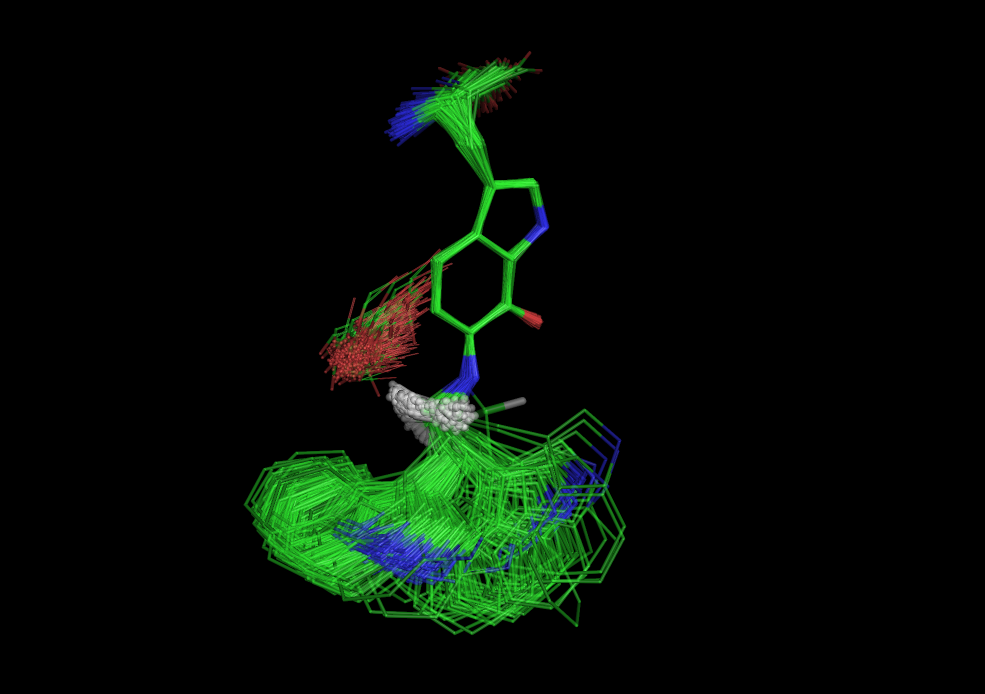
\includegraphics[trim={1cm, 0, 1cm, 0}, clip=True]{chapters/aadh/figures/as_h_wiggle.png}
    }
    \label{fig:ttw_wiggle}
\end{figure}

In summary, the two active sites show distinct differences in the accessible conformations due to the missing di-sulphide bridge between residues Cys81 and Cys113. The two sites are differentiated in three main ways. First, the relevant interatomic distances and hydrogen bonds between TTW and Asp128 in the H but not in the D active site, are consistent with the QM/MM results. Second, the orientation of the NT-C1 bond is syn the C---O7 carbonyl bond in the D active site, whereas in the H active site and QM/MM results, it is anti. Third, the H site is more constrained with less variation in the available conformations compared to the  D active site. These apparent compatibility of the H active site with QM/MM results are surprising given the missing di-sulphide bridge occurs in the H active site. Despite this, only the  coordinate trajectories for the D active site will be used in all further analysis.  

\section{Estimating $\tau$ and $k$}\label{sec:aadh_msm}

The conformational dynamics and metastable states of the active site of AADH will be explored later chapters. In particular, chapter \ref{chap:msm} will detail the how to choose the trajectory pre-processing choices (hyper-parameters) to estimate an optimal MSM. This requires fitting and evaluating a number of MSMs which in turn requires the specification of a Markov lag time ($\tau(\mathrm{MSM})$) and the number, $k$, of dominant eigenvalues. 

In order to estimate these two values for AADH the eigenvalue and implied timescale spectra, resulting from a single set of pre-processing choices, were investigate. The following results are for the D active site only, given the error in the H active site simulation. A similar analysis, albeit with different conclusions, was originally performed for the H site, these are not described. 

The trajectories were discretized by first projecting the cartesian coordinates onto a set of features, applying TICA to reduce the dimension of the feature space and then clustering the frames into a small set of discrete states.  The features used were the bond lengths identified in \cite{ranaghanInitioQMMM2017} i.e. those whose histograms are depicted in panels (a) - (f), (g), (i), (k), (l), (o) of figure \ref{fig:bond_dist}. The intra-molecular hydrogen bonds in panel (h) were excluded due to their small variance. The trajectories were sub-sampled resulting in a time step of $\SI{0.1}{\nano\second}$. TICA was applied with a lag time of $\tau=\SI{1}{\nano\second}$ and the number of components retained set so as to retain $\SI{95}{\percent}$ of the variance which equated to $m=10$ components retained. The k-means clustering was used to cluster the trajectories into $n=\lfloor\sqrt{N}\rfloor = 316$ discrete states. This was based on the heuristic described in \cite{husicWardClusteringImproves2017a} where $N$ is the number of MD frames.  

The Markov lag time must be chosen large enough so that the Markov assumption holds. This equates to the implied timescales ($t_{i}=-\sfrac{\tau(\mathrm{MSM})}{\ln{|\lambda_{i}|}}$) being independent of $\tau(\mathrm{MSM})$. However, the eigenvalue spectrum will be heavily influenced by choice of hyper-parameters, in particular the protein feature. So a suitable lag time for this particular set of hyper-parameters may not prove suitable for another set. In other words, a suitable lag time cannot be chosen independent of the hyper-parameters, but the hyper-parameters cannot be optimised without specifying a lag time. The same reasoning also applies to the number of dominant eigenvalues, except that the number of dominant processes determines the number of eigenvalues used in the VAMP-2 score. 

\begin{figure}
    \centering
    \mycaption{The implied timescales and relative VAMP-2 scores as a function of the Markov lag time $\tau(\mathrm{MSM})$. The TICA lag time was set to $\tau=\SI{1}{\nano\second}$, with \SI{95}{\percent} of the variance retained meaning $m=10$ components were retained. The number of cluster centres was set to $n=316$. Panel (a) shows the first five implied timescales for $\SI{0}{\nano\second} < \tau(\mathrm{MSM}) < \SI{5}{\nano\second}$, panel (b) shows the first five implied timescales for $\SI{0}{\nano\second} < \tau(\mathrm{MSM}) < \SI{50}{\nano\second}$. The solid lines and coloured shaded areas are the mean and \SI{95}{\percent} credible intervals respectively, estimated using MCMC with $500$ posterior samples. The grey shaded area is the region for which the implied timescales are smaller than the lag time. Panel (c) and (d) show the VAMP-2 scores, scored on the first $2-5$ eigenvalues for the same ranges. The VAMP-2 scores are indexed to $1$ at their initial value. The colour coding is consistent between the implied timescale plots and VAMP-2 plots. So that $k=2$, in blue, is the score including the first eigenvalue $\lambda = 1$ and the eigenvalue of the longest implied timescale also shown in blue in panels (a) and (b). }
    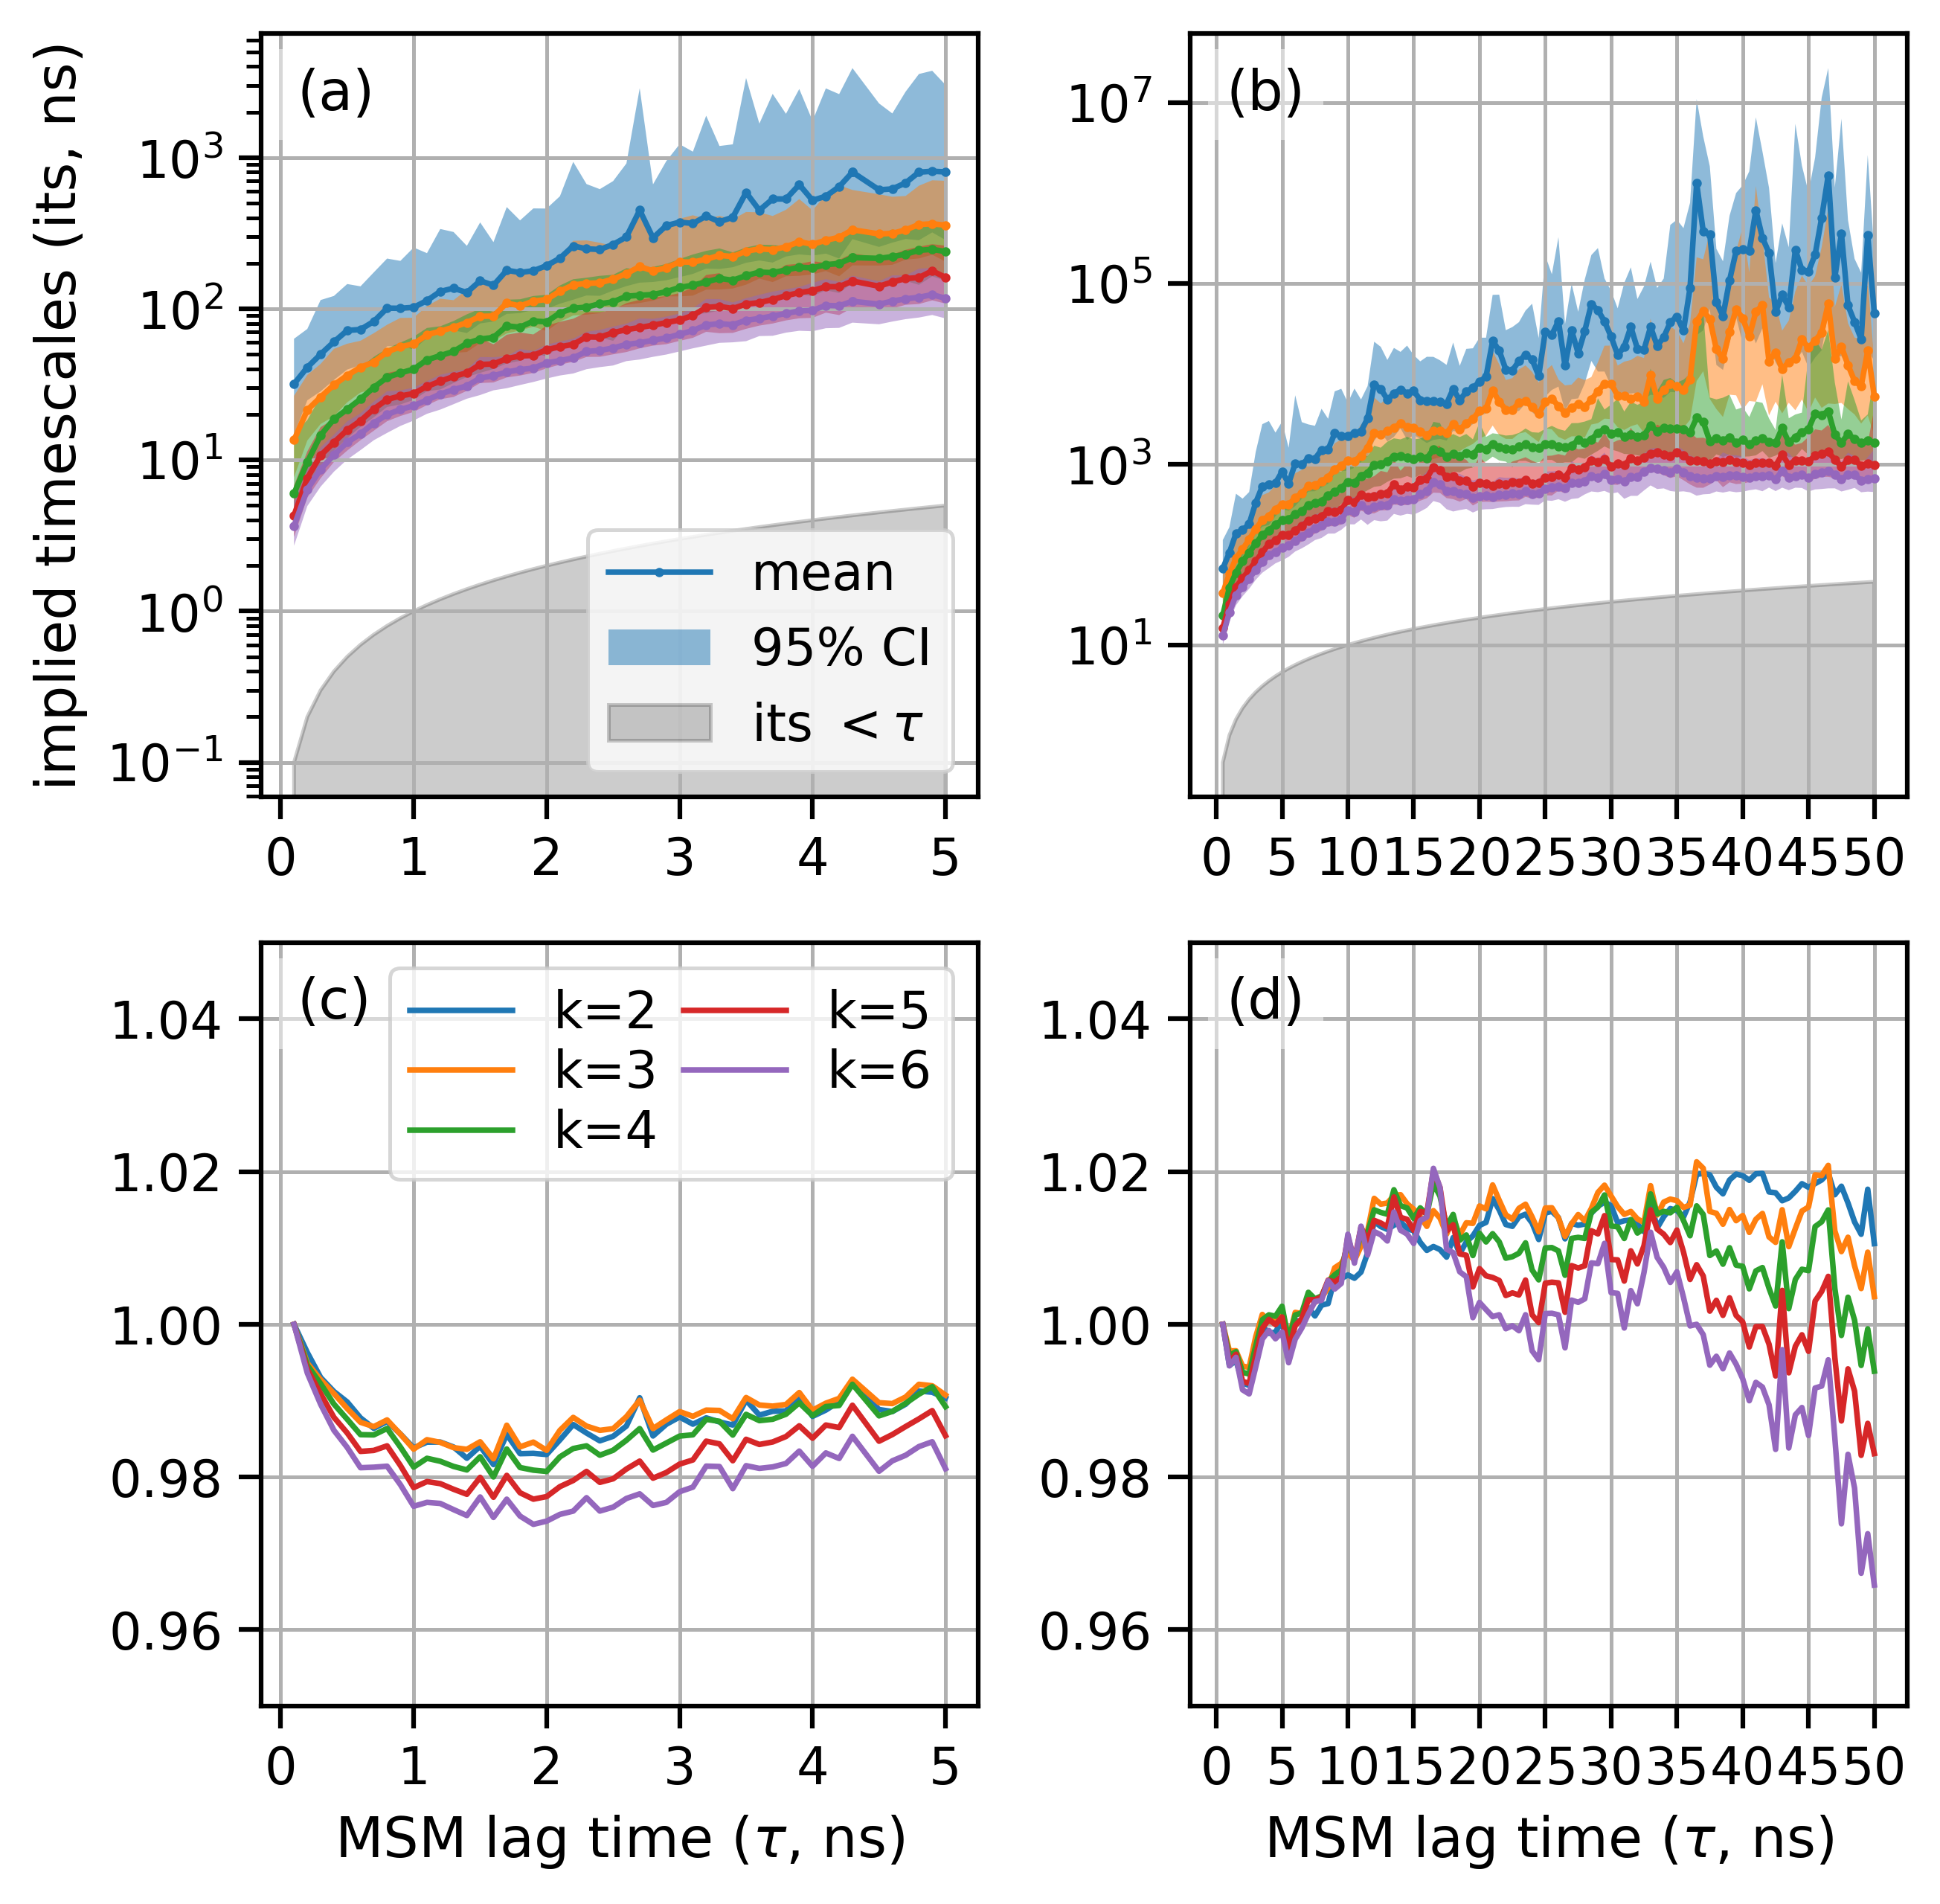
\includegraphics[width=0.8\textwidth]{chapters/aadh/figures/implied_timescales_D.png}
    \label{fig:its_d}
\end{figure}

A way out of this circular reasoning problem can be found by noting the following. First, the purpose of specifying the lag time and number of dominant processes is to provide a starting point from which the hyper-parameters of the MSM will be optimised. It is therefore only necessary that the choices do not affect the optimisation, rather than provide a strictly valid MSM specification. The lag time and number of dominant processes has only a small effect on the value of the VAMP-2 score as demonstrated by figure \ref{fig:its_d}. The first five implied timescales are shown a panel (a)  for $\SI{0}{\nano\second} < \tau(\mathrm{MSM}) < \SI{5}{\nano\second}$) and panel (b) for $\SI{0}{\nano\second} < \tau(\mathrm{MSM}) < \SI{50}{\nano\second}$. Underneath in panels (c) and (d) are shown the VAMP-2 scores with $k$ ranging from $2$ to $5$, which correspond to successively including the implied timescales shown in panels (a) and (b). The implied timescale (shown in blue) appears to become independent of the lag time from approximately \SI{10}{\nano\second}. However as panels (c) and (d) show the lag time has little effect on the VAMP-2 scores which vary by less than $\pm\SI{4}{\percent}$ from their initial values over all lag times. The value of $k$ also has little effect on VAMP-2 scores, at least up to $\tau(\mathrm{MSM})=\SI{15}{\nano\second}$ where their relative values start to diverge. Third, a  value of $\tau(\mathrm{MSM})$ and $k$ used for inference can be determined after optimisation through appropriate sensitivity analysis. A value of $\tau(\mathrm{MSM})=\SI{2}{\nano\second}$ was chosen based on the relatively small variation of the VAMP-2 score (panel (c) of figure \ref{fig:its_d}) and the larger number of observations that a small value affords. 

\begin{figure}
    \centering
    \mycaption{The ratio of successive implied timescales for a Markov state model with $\tau(\textrm{MSM})=\SI{2}{\nano\second}$, estimated using MCMC with $1000$ posterior samples. The TICA lag time was set to $\tau=\SI{1}{\nano\second}$, with \SI{95}{\percent} of the variance retained meaning $m=10$ components were retained. The number of cluster centres was set to $n=316$. The blue dots and error bars are the mean and \SI{95}{\percent} credible intervals.}
    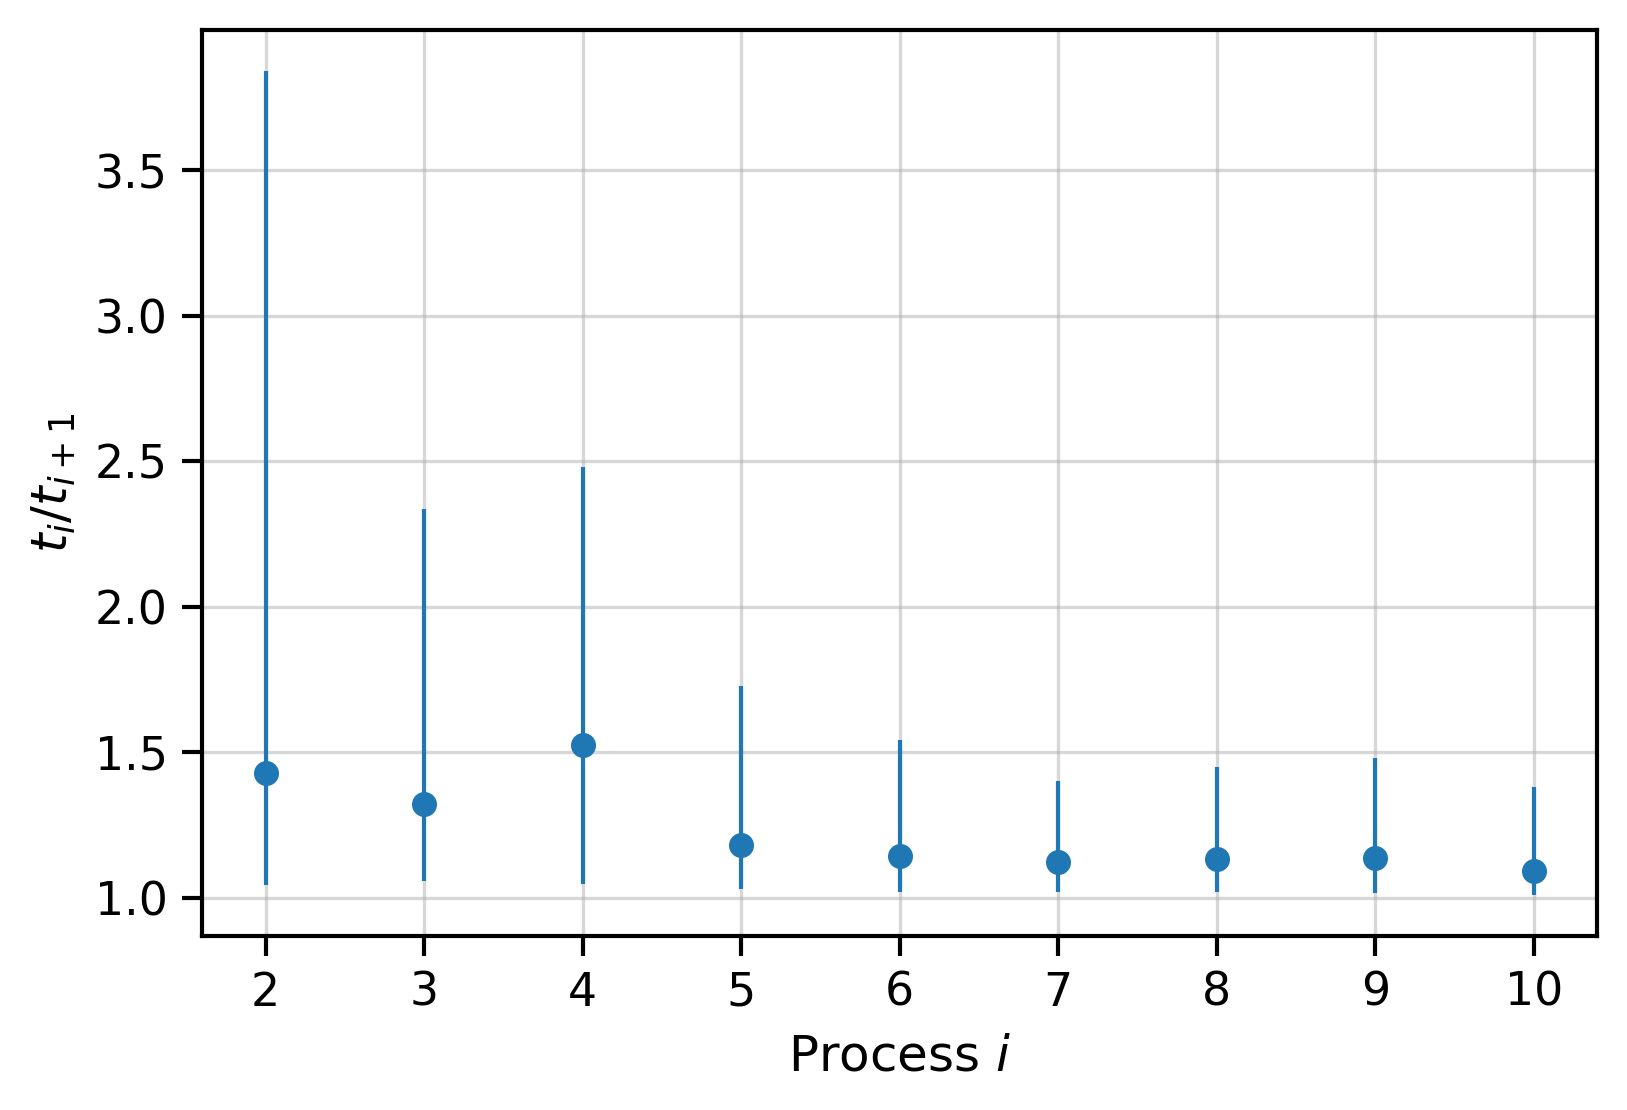
\includegraphics[width=0.8\textwidth]{chapters/aadh/figures/timescale_ratios_D.png}
    \label{fig:ts_ratios_d}
\end{figure}

The number of dominant processes was determined by inspection of the relative gaps in the eigenvalue spectrum at $\tau(\mathrm{MSM})=\SI{2}{\nano\second}$ shown in figure \ref{fig:ts_ratios_d}. The largest gap in the eigenvalues is between the fourth and fifth relaxation process. Therefore a value of $k=4$ was used. 

An alternative analysis was performed using a value of the TICA lag time set to $\tau=\SI{10}{\nano\second}$ with \SI{95}{\percent} of the variance retained meaning $m=8$ components were retained. The same number of cluster centres, $n=316$ was used. The implied timescale plots are shown in figure \ref{fig:its_d_sens}, these results do not change the Markov lag time suggestion of \SI{2}{\nano\second}. The ratio of implied timescales for an MSM with $\tau(\textrm{MSM})=\SI{2}{\nano\second}$ is shown in figure \ref{fig:ts_ratios_d_sens}. These suggest a single dominant relaxation process, i.e., $k=2$. The higher value of $k=4$ is retained however on the basis that including extra, potentially fast timescales processes in the definition of $\operatorname{VAMP-2}$ will not significantly affect the optimisation results. The issue of whether this is an appropriate value will be further investigated in the sensitivity analyses of chapter \ref{chap:msm} and in chapter \ref{chap:hmm} where the issue of the number of metastable states implied by a MSM will be addressed quantitatively. 

{\huge This has been copied `as-is' from chapter \ref{chap:msm}}
\section{MSM Optimisation}\label{subsec:aadh}

Having explored the use of response surfaces and Bayesian optimisation in the well known alanine dipeptide system with a two-dimensional hyper-parameter space. These techniques were applied to the unknown case of the active site of AADH. 

[TM: give summary of what's coming next]

\subsection{Response surface}\label{subsubsec:aadh_rsm}

\begin{figure}[p]
    \centering
    \mycaption{The $\operatorname{VAMP-2}$ scores of the hyperparameter trials for MSMs of AADH. The test response, $f^{test}=f\left(\chi, \tau, m, n; \mathbf{X}^{test}\right)$, is shown in blue, for (a) the $\phi, \psi, \chi$ torsions, (c) all distances between heavy atoms, (e) alpha-Carbon contact distances, (g) heavy atom contact distances, (i) root mean square deviation of heavy atoms. The difference between $f^{train}$ and $f^{test}$ is shown in orange for (b) the the $\phi, \psi, \chi$ torsions and so on. The horizontal axis is the rank of the trial according to the test score. Each trial was scored with $20$ iterations of 50:50 shuffle split cross-validation. The error bars represent the 25th and 75th quantiles of the cross-validation folds. The features are ordered according to the mean of the their test scores.}
    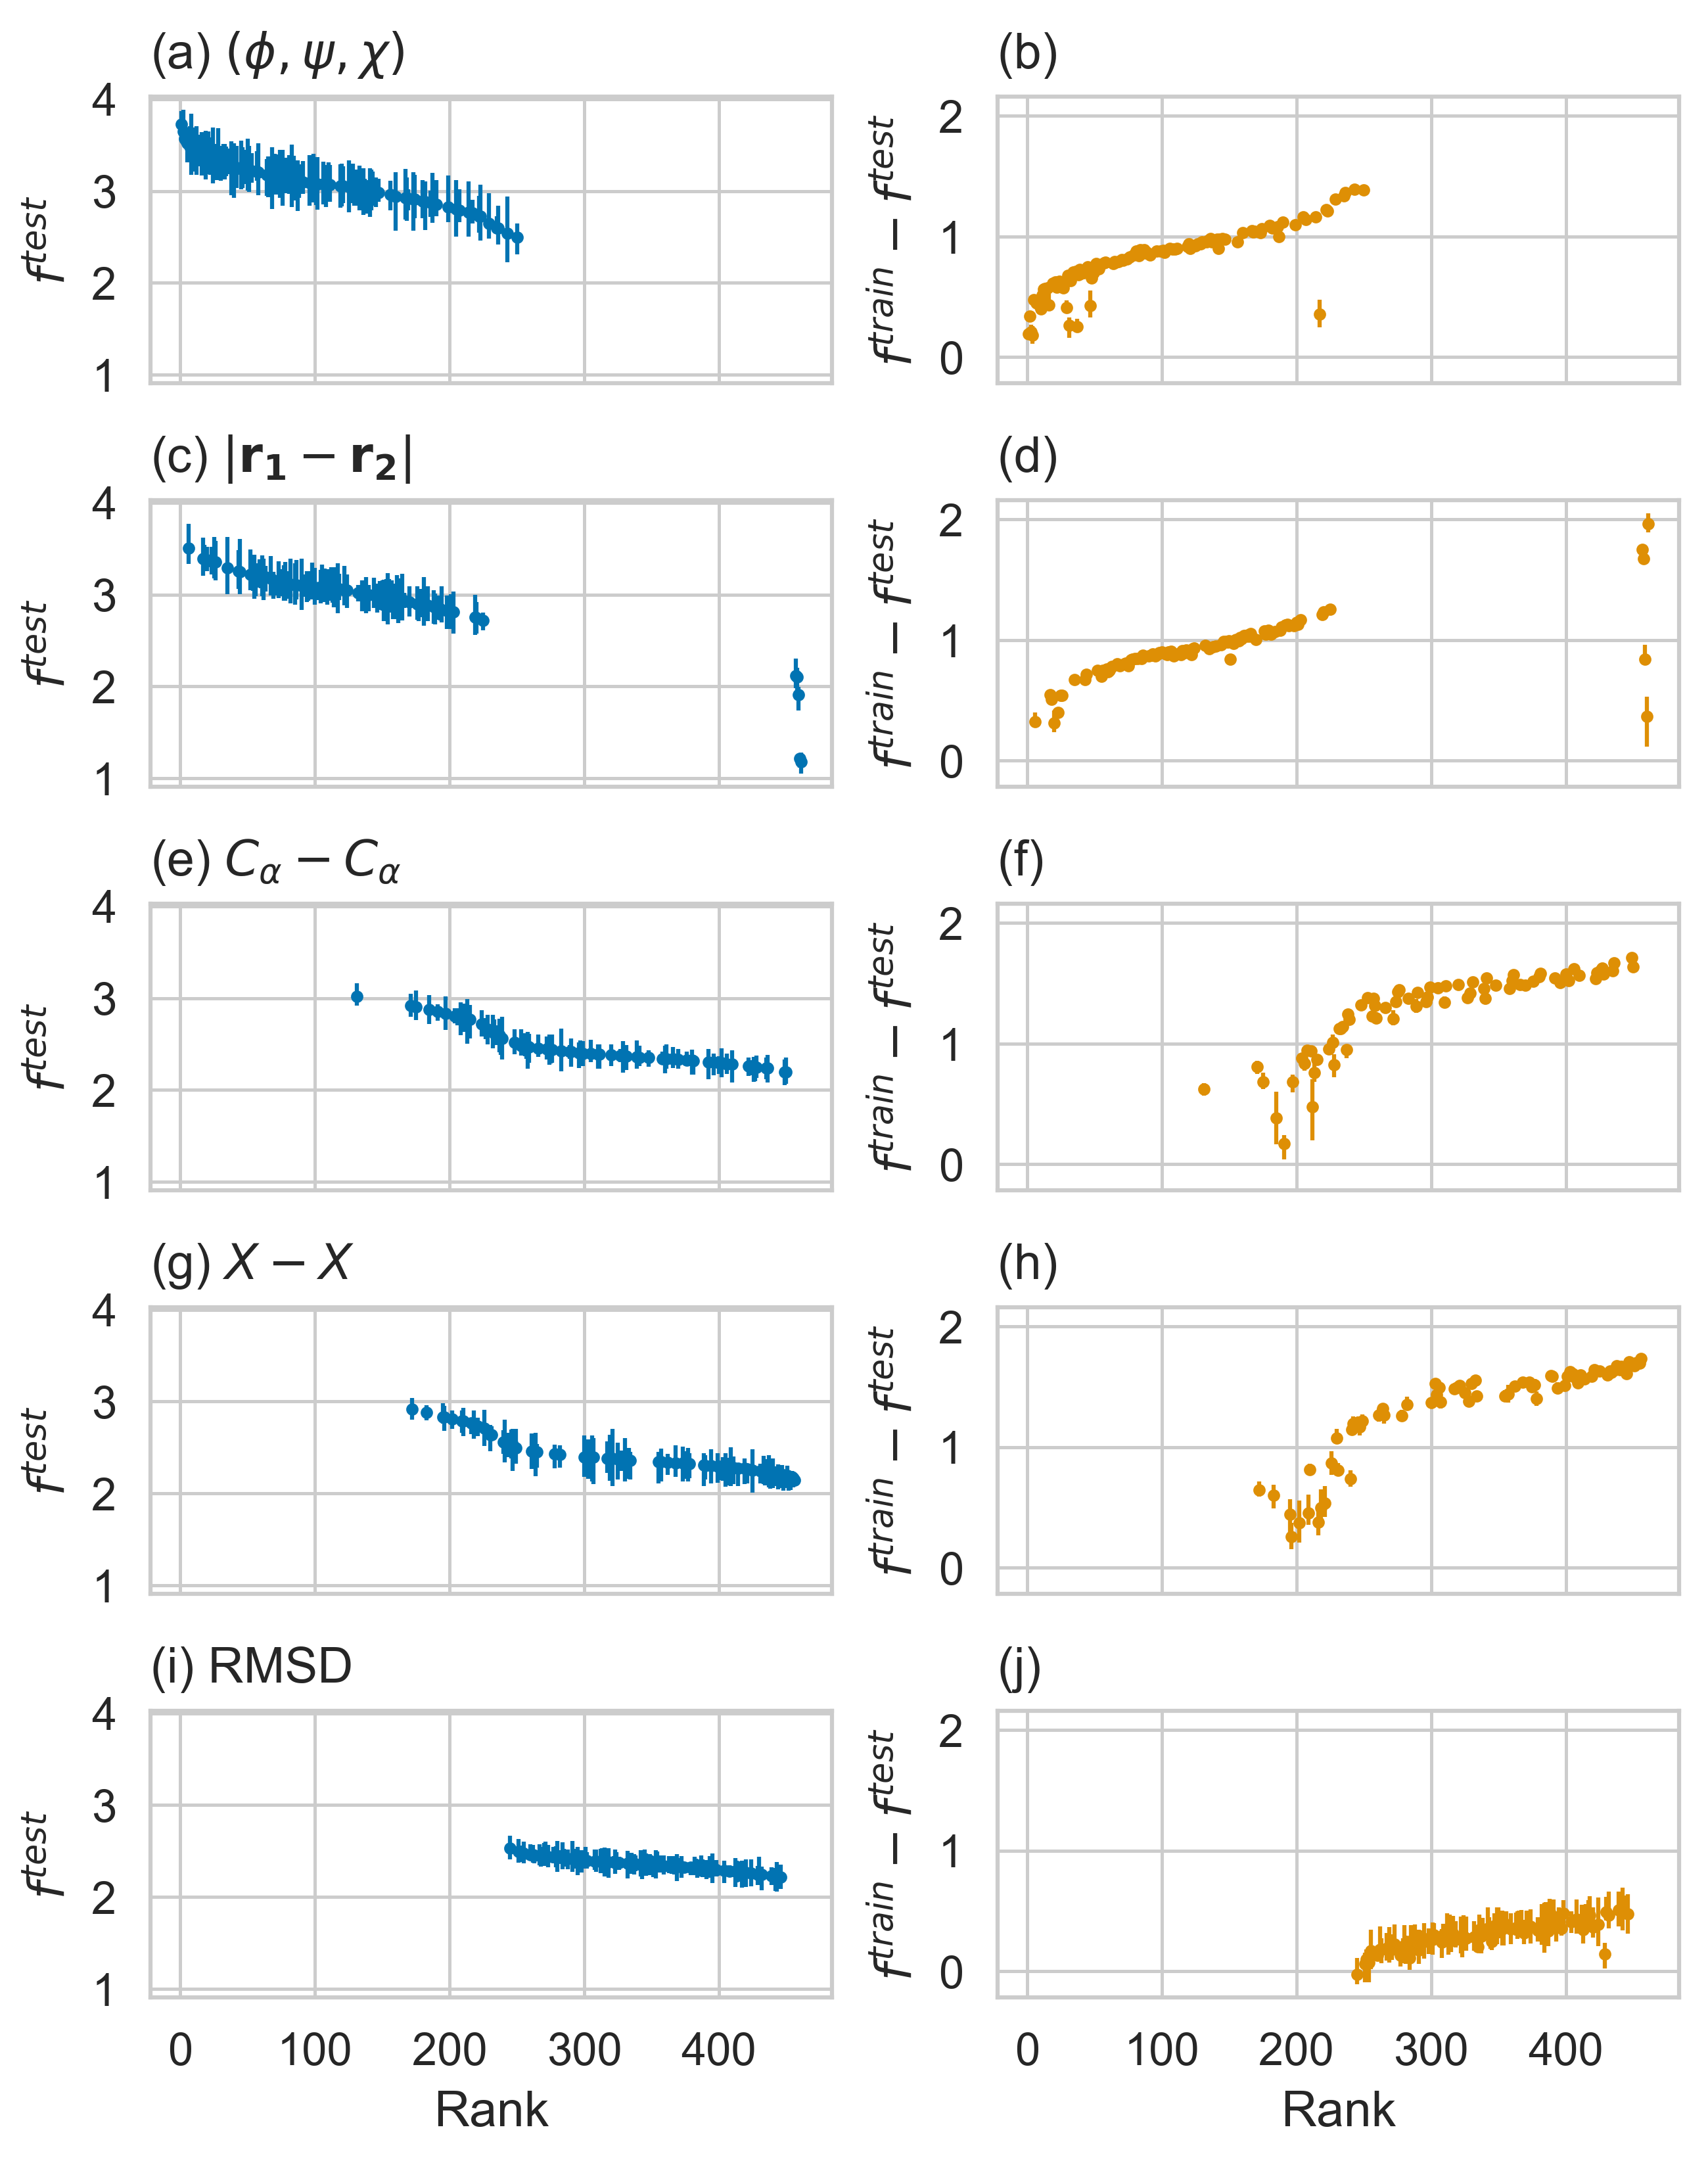
\includegraphics[width=0.8\textwidth]{chapters/msm_optimization/figures/aadh_train_test_results.png}
    \label{fig:aad_train_test}
\end{figure}

The mean MSM response for the randomly sampled hyper-parameter trials are shown in  figure \ref{fig:aad_train_test} with the test response shown in blue and the difference between the training and test response shown in orange.  The panels correspond to the value $\chi$ and are ordered according to their average of the test responses. The horizontal axis is the rank of the trial determined by their test response. There is clear range of response values in the range $2 < \operatorname{VAMP-2} < 4$ with the $(\phi, \psi, \chi)$ torsions  (panel (a)) and the interatomic distances feature ( $\left|\mathbf{r}_{1}-\mathbf{r}_{2}\right|$) (panel (c)) both performing the best out of the five features. 

In contrast to the case of alanine dipeptide, all features show a marked degree of over-fitting $\Delta f$. However, within each feature there are combinations of the remaining hyper-parameters for which $\Delta f=0$ implying that it is possible to create a consistent picture of relaxation processes which generalize well for each feature. The response of the $(\phi, \psi, \chi)$ feature  approaches the maximum response of $VAMP-2 = 4$ for the highest ranked trials, indicating the possibility of the three slow relaxation processes. 

\begin{figure}
    \centering
    \mycaption{[TM: label with Pearson R for each panel?] Goodness of fit for the response surface of AADH conditional on each feature. The horizontal axis ($y$) are the observed trial values and the vertical axis is the mean response ($f(\mathbf{x})$). The error bars are $\pm 2\sigma$ where $\sigma$ is the standard deviation of the response surface including the noise term $\sigma_n$.}
    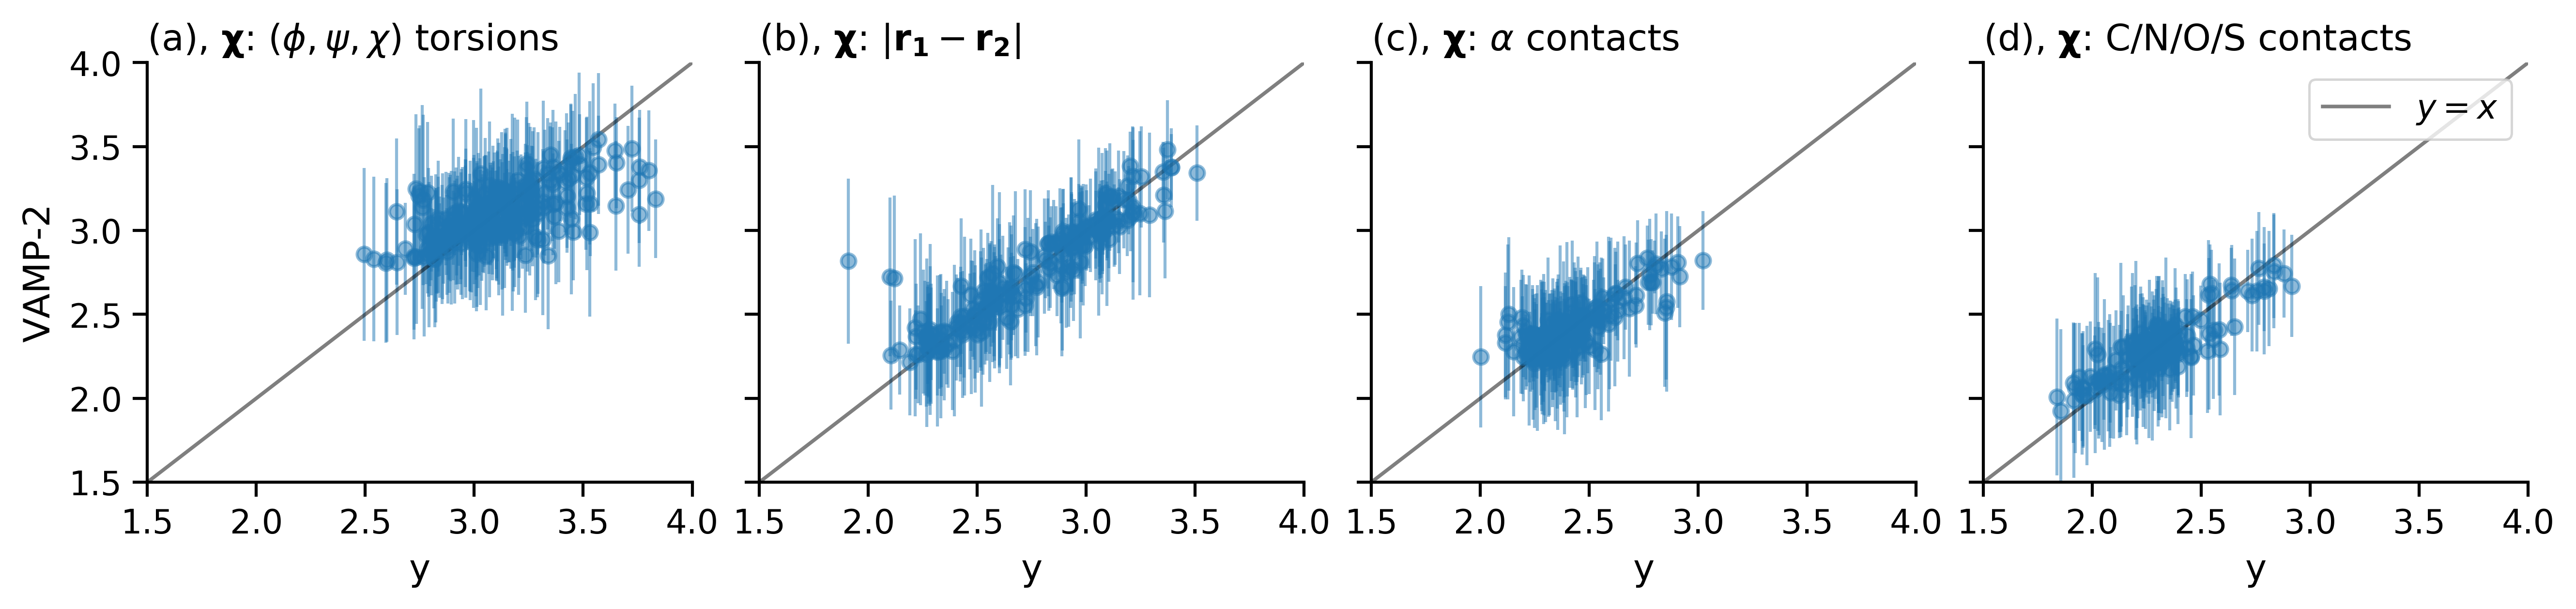
\includegraphics[width=0.8\textwidth]{chapters/msm_optimization/figures/aadh_response_surface_fit_d.png}
    
    \label{fig:aadh_rsm_fit}
\end{figure}

The response surface as a function of the feature, $\chi$, TICA lag time, $\tau$, number of TICA components retains $m$, and the number of cluster centres, $n$ was estimated with a GP. The RMSD feature was left out of the response surface because the $\tau$ and $m$ hyper-parameters do not apply, creating a \emph{conditional} search space [] which  poses problems GP although there are attempts to mitigate this []. While this is a problem in general for this method, the poor performance of RMSD as a feature both here and in alanine dipeptide mean that this will not affect finding the optimum hyper-parameters. 

[TM: how are kernel and input warping chosen?] Model selection on the kernel and input warping revealed an exponential kernel (equation \ref{eqn:kern_exp}) and a linear input transformation for $\tau, m$ and $n$ were most appropriate, with an MSLL of $-0.01298$ and a SMSE of $0.3087$ (see table \ref{tab:aadh_rsm_metrics_all_data} for the other models' selection metrics). A more intuitive assessment of the fit of the can be found in figure  \ref{fig:aadh_rsm_fit} which shows the observed and predicted values for each feature. There is clearly a good fit for all the features except for the $(\phi, \psi, \chi)$ torsions where the predicted values are slightly under/over estimated for the highest/lowest values with this feature. This creates the possibility of a false bimodal response surface which must be checked when determining the optimal hyper-parameters.  The relatively poor fit on this feature is likely due to the fully multiplicative nature of the kernel. More flexible kernels (as discussed in e.g. \cite{duvenaud2011additive}) which model lower order interactions may be able to overcome this problem. 

\begin{figure}
    \centering
    \mycaption{The relevance of the hyper-parameters of AADH. The distribution of the parameters of the response surface were estimated using MCMC. The relevance of the features (levels of $\chi$) are shown in blue, labelled `Feature'. The relevance of the the other hyper-parameters are shown in orange, labelled `Other'.}
    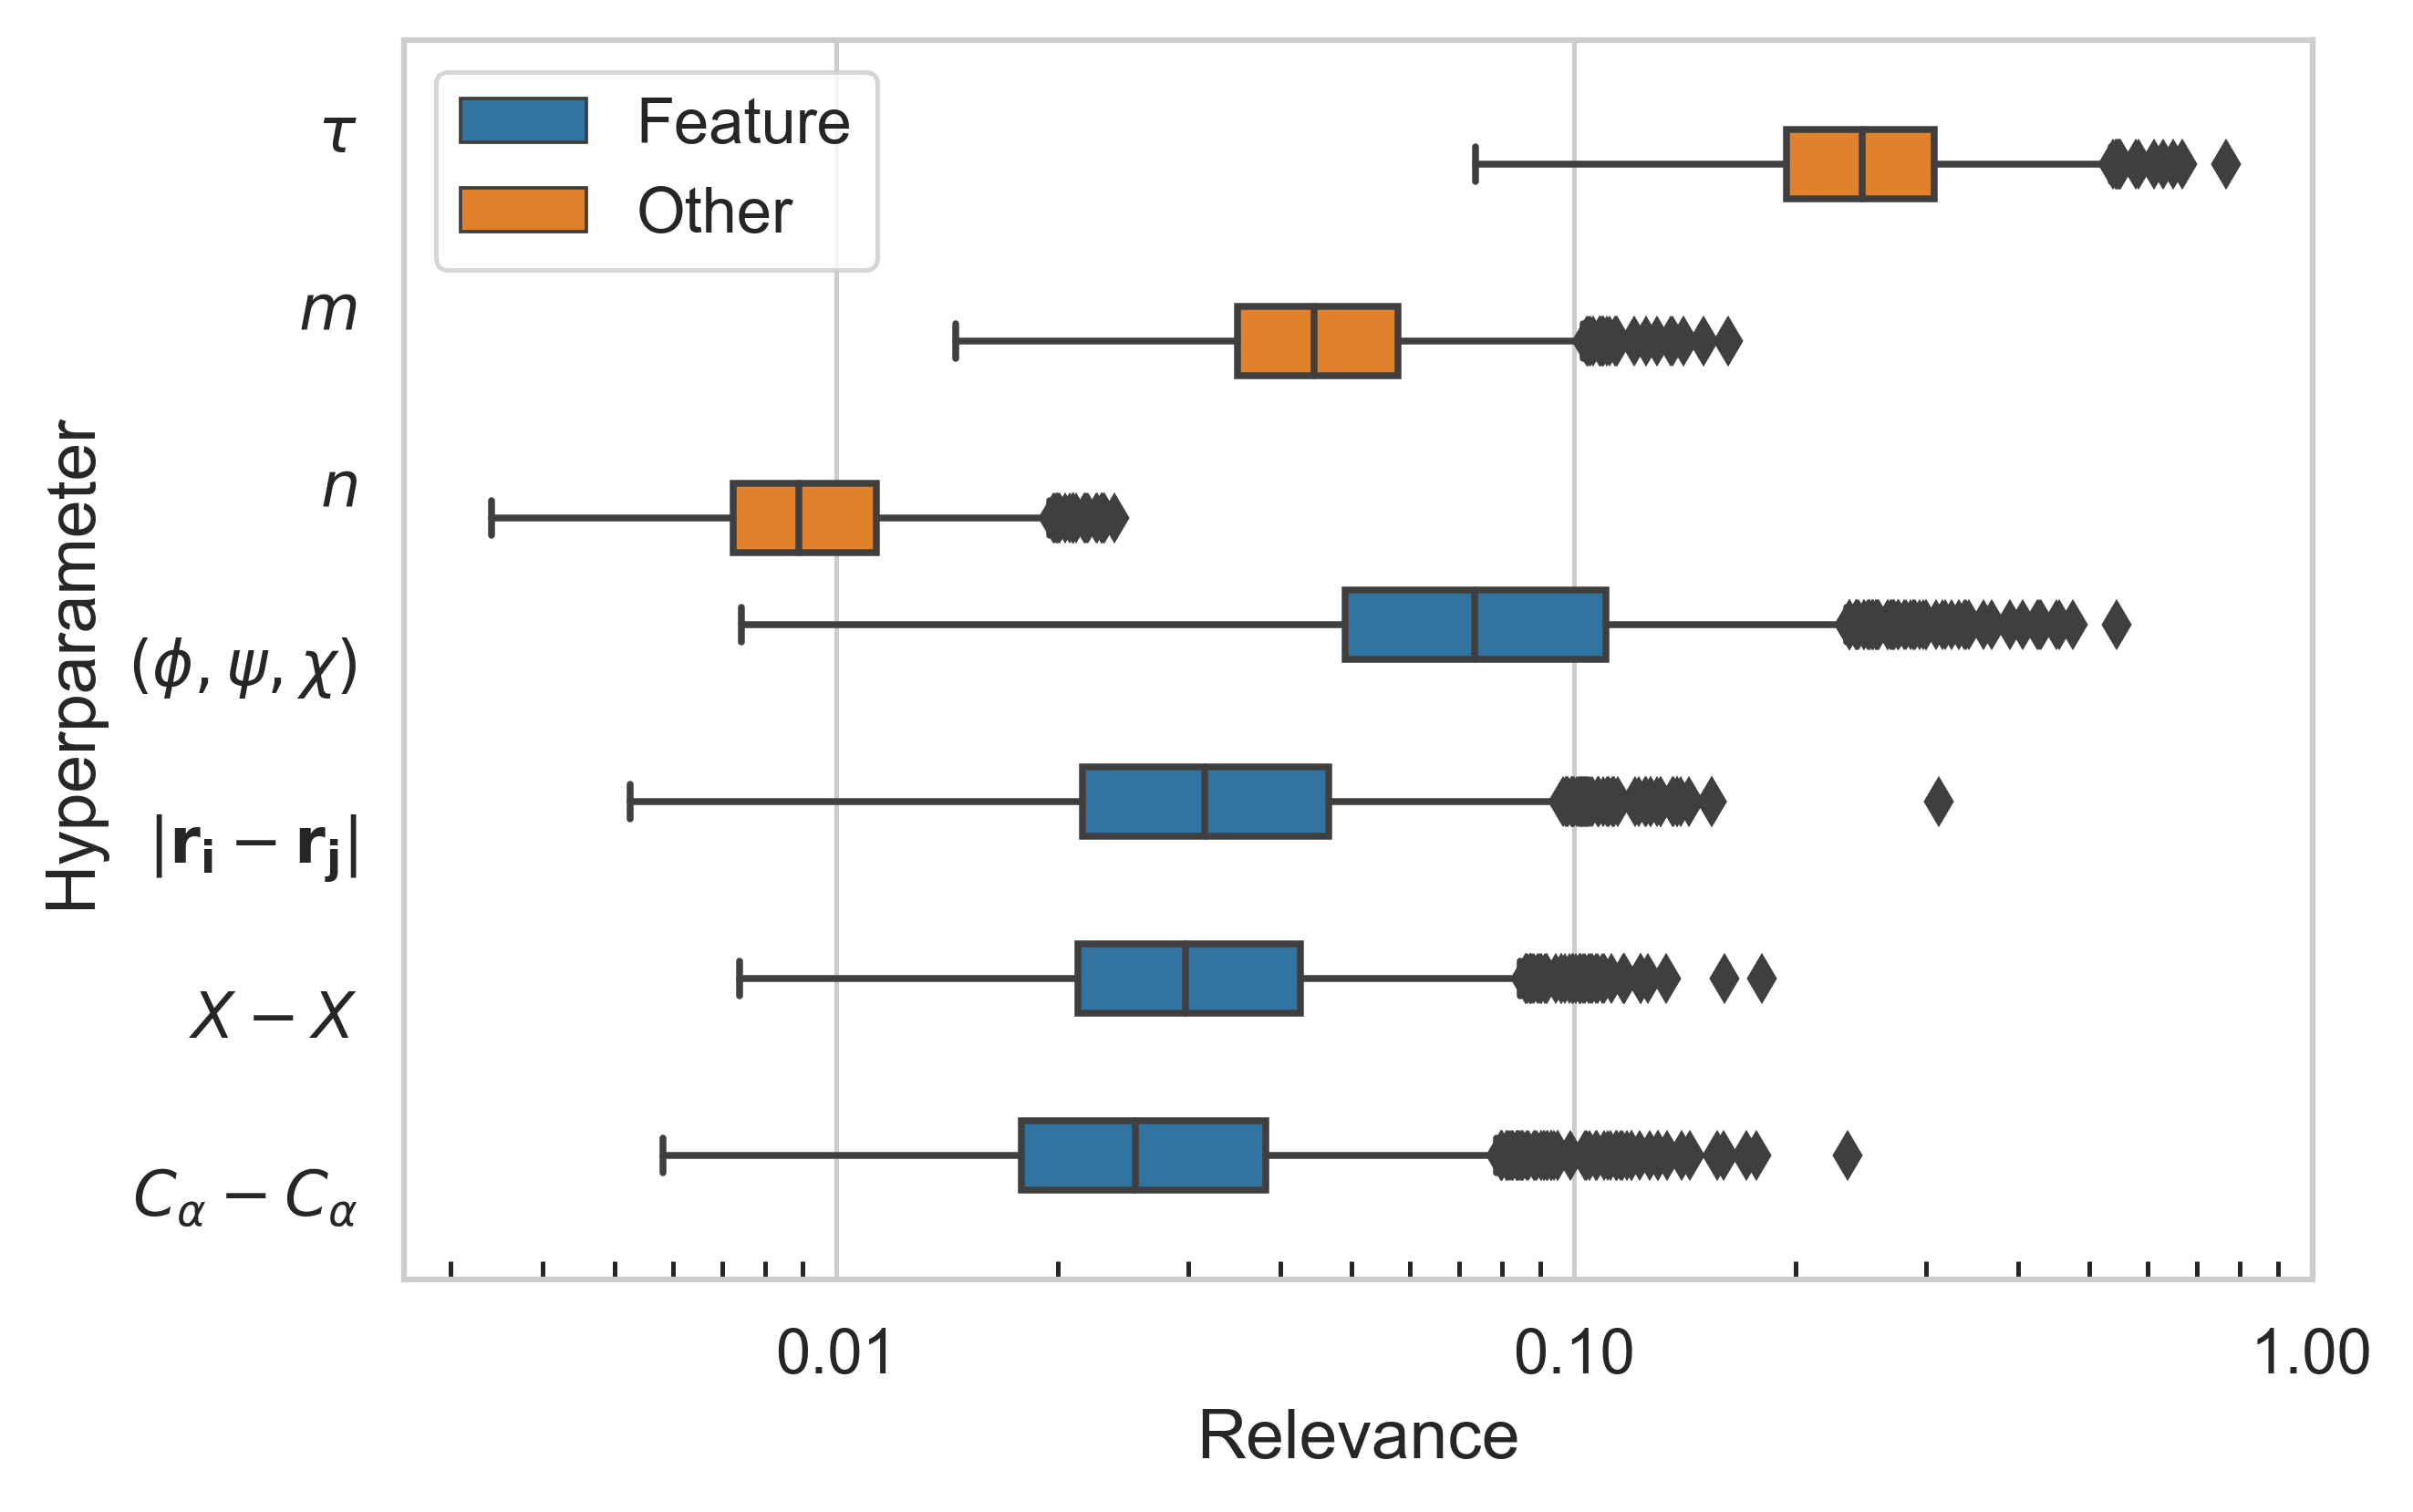
\includegraphics[width=0.8\textwidth]{chapters/msm_optimization/figures/AADH_relevance_d.png}
    \label{fig:aadh_relevance}
\end{figure}

\begin{table}
    \centering
    \mycaption{Median and $\SI{95}{\percent}$ credible intervals for the kernel hyper-parameters of the AADH response surface estimated using MCMC. The length-scale parameters in equation \ref{eqn:kernel_form} are re-written here as relevances.}
    \begin{tabular}{|l|r|l|}
    \hline
                             Hyper-parameter &  Median &     (95\% C.I.) \\
    \hline\hline
                    $R_{(\phi, \psi, \chi)}$ &   0.073 &  (0.021-0.248) \\
     $R_{|\mathbf{r_{1}} - \mathbf{r_{2}}|}$ &   0.032 &  (0.012-0.098) \\
                 $R_{C_{\alpha}-C_{\alpha}}$ &   0.025 &  (0.009-0.084) \\
                                   $R_{X-X}$ &   0.030 &  (0.012-0.083) \\
                                  $R_{\tau}$ &   0.246 &  (0.126-0.474) \\
                                     $R_{m}$ &   0.044 &  (0.022-0.095) \\
                                     $R_{n}$ &   0.009 &  (0.005-0.018) \\
                                      $\eta$ &   1.540 &  (1.117-2.154) \\
                                  $\sigma_n$ &   0.011 &  (0.001-0.035) \\
    \hline
    \end{tabular}
    \label{tab:aadh_rel}
\end{table}

The multidimensional nature of the response surface poses problems for visualisation and for understanding the interaction between the hyper-parameters in determining the response. However, calculating the hyper-parameter relevance can help by suggesting the displayed granularity of the inputs. Figure \ref{fig:aadh_relevance} shows the posterior distribution of relevance for the features (blue) and the remaining hyper-parameters (orange). The median and $\SI{95}{\percent}$ credible intervals are tabulated in table \ref{tab:aadh_rel}. 

Figure \ref{fig:aadh_rsm} shows  a projection of the response surface, $f(\mathbf{x};\mathcal{D}_{361})$, informed by the relevance. $\tau$ and $m$ are the two highest relevance hyper-parameters ($R_{\tau} = 0.246 (0.126-0.474)$, $R_{m} = 0.044 (0.022-0.095)$) so the response surface is shown as a 2D heat map with $\tau$ on the vertical and $m$ on the horizontal axis. Only odd values of $m$ are shown given the slightly lower relevance of this feature. The number of cluster features is, like the case of alanine dipeptide, the lowest relevance hyper-parameter ($R_{n} = 0.009 (0.005-0.018)$ and so heat maps for only two value of $n$ are shown: the value at the maximum of the response surface ($n=207$ although the value displayed is rounded to $210$) and $n=1000$. With only four features, it is  simple to show the response surface for each of them. With a larger number of features, displaying the high relevance features and \emph{only one} of the low relevance features would be sufficient. This is clearly borne out with this surface - the two lower relevance features, the contact distances, are very similar and including both in the visualisation is redundant. However, as all features have absolutely low relevance ($R<1$) then their response surfaces are expected to be similar. The maximum of the response surface is shown highlighted in white, occurs at $\mathbf{x}=\left(\chi=(\phi, \psi, \chi), \tau = \SI{12.5}{\nano\second}, m=1, n=207\right)$ with a value of $\mu=3.54 3\pm 0.396$. The features of this response surface will be discussed in the context of sensitivity analysis in later sections. 

\begin{figure}[p]
    \centering
    \mycaption{The response surface of AADH using the unoptimised hyper-parameter trial data set. For each feature two heat maps are shown for $n=210, 1000$ with $\tau$ on the vertical axis and $m$ on the horizontal axis: for the dihedrals feature panel (a) shows the heat map for $n=210$  and panel (b) shows the heat map for $n=1000$ and similarly for the remaining features. The white star denotes the approximate location of the maximum of the surface, the true maximum occurs at $\tau=\SI{12.5}{\nano\second}, m=1, n=207$  The value of the response surface denoted by the color (lighter implies higher values) and with the text annotations. }
    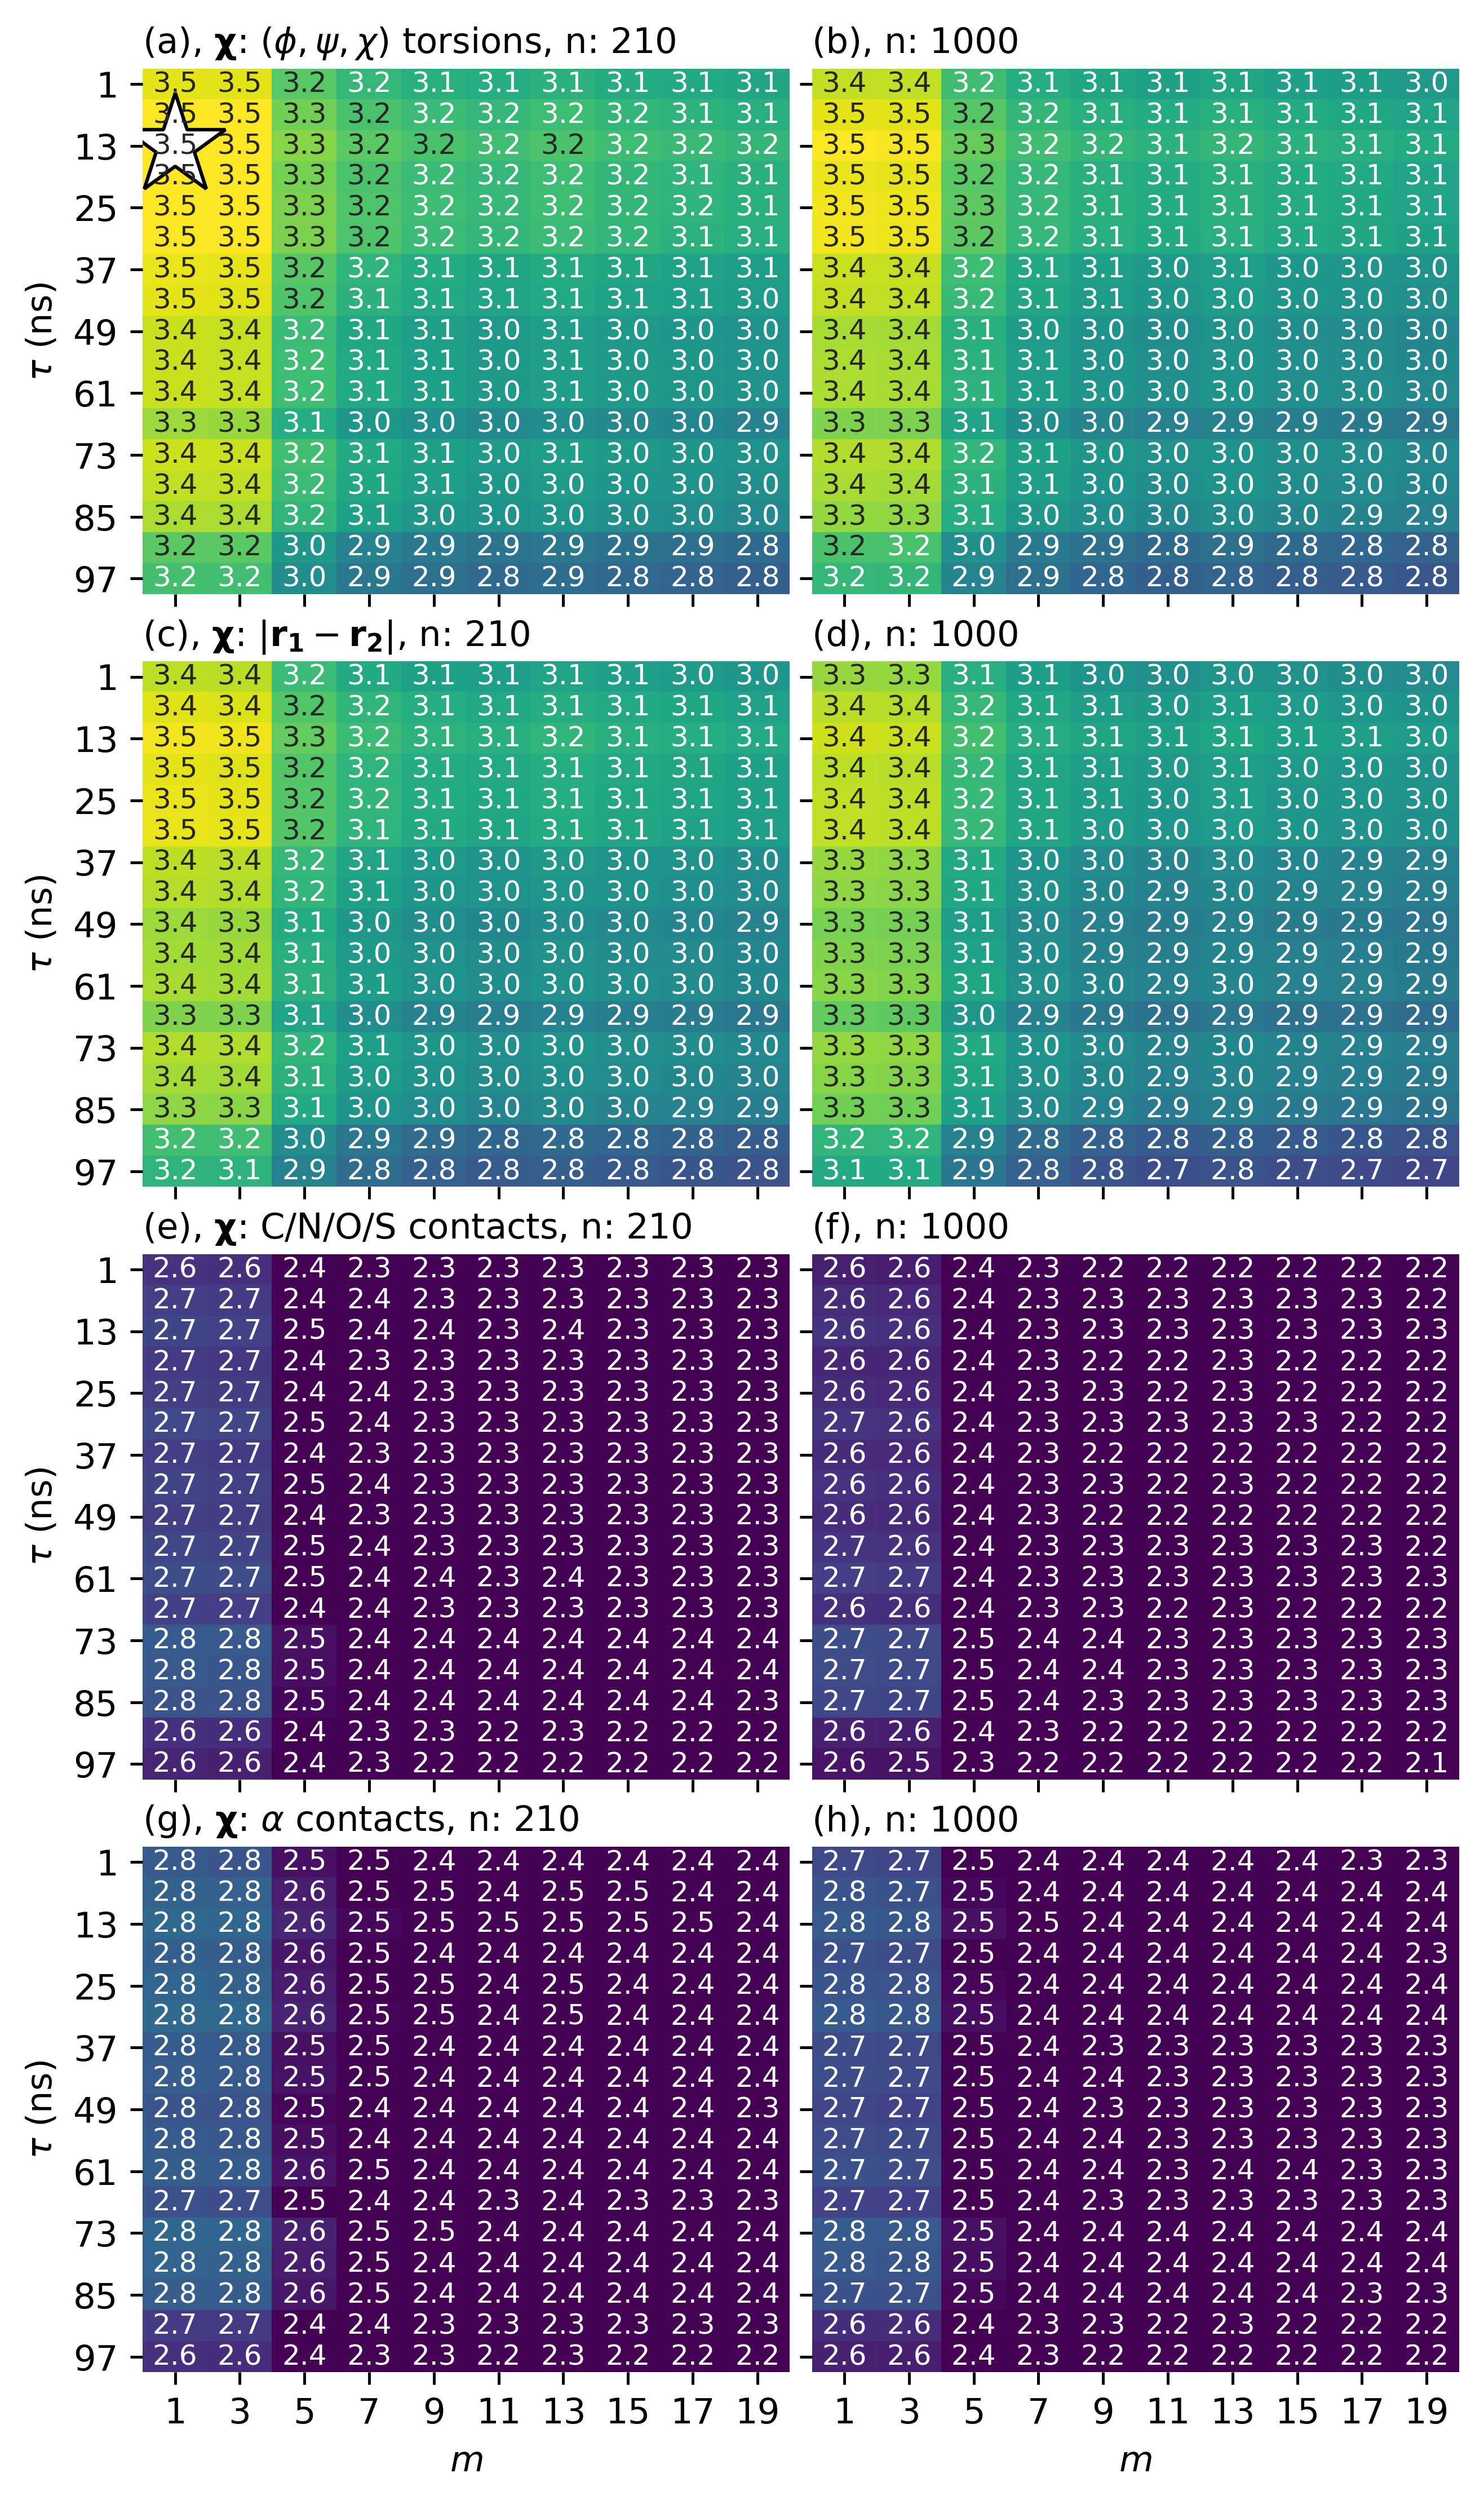
\includegraphics[width=0.7\textwidth]{chapters/msm_optimization/figures/aadh_response_surface_d.png}
    \label{fig:aadh_rsm}
\end{figure}

\begin{table}
    \centering
    \mycaption{Optimum MSM hyper-parameters for AADH pre- and post-Bayesian optimisation (BO). Each column represents a Bayesian optimisation experiment, seeded with $N_{seed}$ randomly sampled hyper-parameter trials. Five iterations of optimisation were run with $N_{seed}=100$ (labelled $\# 1, 2$ etc.) and a single iteration optimising the response surface using all the trial data ($N_{seed}=361$). Each row is a variable or outcome with values associated with the optimum value of $\mu$ before and after the BO.}
    \begin{tabular}{|ll|lllll|l|}
    \hline
    &$N_{seed}$ & 100 & & & & &361\\
    &\#&1&2&3&4&5&1\\
    \hline\hline
    $N_{total}$&Pre&100&100&100&100&100&361\\
    &Post&150&150&150&150&150&410\\
    \hline
    $\mu$&Pre&3.487&3.355&3.599&3.473&3.478&3.543\\
    &Post&3.500&3.558&3.545&3.581&3.569&3.558\\
    \hline
    $\sigma$&Pre&0.152&0.135&0.306&0.234&0.126&0.198\\
    &Post&0.202&0.117&0.101&0.084&0.072&0.091\\
    \hline
    $\chi$&Pre&$(\phi,\psi,\chi)$&$|\mathbf{r_{i}}-\mathbf{r_{j}}|$&$(\phi,\psi,\chi)$&$(\phi,\psi,\chi)$&$|\mathbf{r_{i}}-\mathbf{r_{j}}|$&$(\phi,\psi,\chi)$\\
    &Post&$(\phi,\psi,\chi)$&$(\phi,\psi,\chi)$&$(\phi,\psi,\chi)$&$(\phi,\psi,\chi)$&$(\phi,\psi,\chi)$&$(\phi,\psi,\chi)$\\
    \hline
    $\tau$&Pre&51.0&57.8&12.5&12.5&18.0&12.5\\
    &Post&1.0&4.0&3.0&1.0&1.0&10.0\\
    \hline
    $m$&Pre&1&3&1&1&1&1\\
    &Post&2&1&2&1&1&2\\
    \hline
    $n$&Pre&396&234&207&207&79&207\\
    &Post&10&180&10&230&540&310\\
    \hline
    \end{tabular}
    \label{tab:aadh_opt_results}
\end{table}

In order to test the convergence of the maximum of $f(\mathbf{x}; \mathcal{D}_{361})$, $50$ steps of Bayesian optimisation was performed. The values of the response and associated hyper-parameters pre- and post-optimisation (i.e. $f(\mathbf{x}; \mathcal{D}_{361})$ and $f(\mathbf{x}; \mathcal{D}_{410})$) are tabulated in table \ref{tab:aadh_opt_results}. The optimisation resulted in a small improvement in the response from $\mu=3.543 \pm 0.396 \rightarrow 3.558 \pm 0.182$ (a $\SI{0.4}{\percent}$ improvement) with no change in the optimum feature ($(\phi, \psi, \chi)$ dihedrals) and only small changes in the other hyper-parameters.  

In order to see whether this maximum could be reached with a fewer number of trials, five response surfaces fit on random subsets of the trial data with $100$ observations, $f^{i}(\mathbf{x};\mathcal{D}_{100}), i = 1 - 5$, were optimized with $50$ steps of Bayesian optimisation. The kernel and input warping for $f^{i}(\mathbf{x};\mathcal{D}_{100})$ were determined for each $i$ separately. The model selection metrics for each combination of kernel and input warping are tabulated in tables \ref{tab:aadh_rsm_metrics_iter_1} - \ref{tab:aadh_rsm_metrics_iter_5}. The results of the optimisation trials are shown in table \ref{tab:aadh_opt_results} and the incumbent trajectories are shown in are shown in figure \ref{fig:aadh_opt_traj_d}. Also shown in figure \ref{fig:aadh_opt_traj_d} are the maximum of the response surface $f(\mathbf{x};\mathcal{D}_{361})$ shown as orange lines, and the maximum of $f(\mathbf{x};\mathcal{D}_{410})$ shown as blue lines. 

\begin{figure}[p]
    \centering
    \mycaption{The Bayesian optimisation trajectories for AADH. Each column shows the trajectories of the incumbent $\mu\pm 2\sigma$ (panels (a) - (e)), and the accompanying value of: $\chi$ (panels (f) - (j)), $m$ (panels (k) - (o)), $\tau$ (panels (p) - (t)) and $n$ (panels (u) - (y)). The location of the final value of the trajectory is highlighted with a black star. For reference the corresponding values determined from the response surface using all the hyper-parameter trials are shown as solid horizontal lines: the response surface before optimisation are shown in orange and after Bayesian optimisation in blue.}
    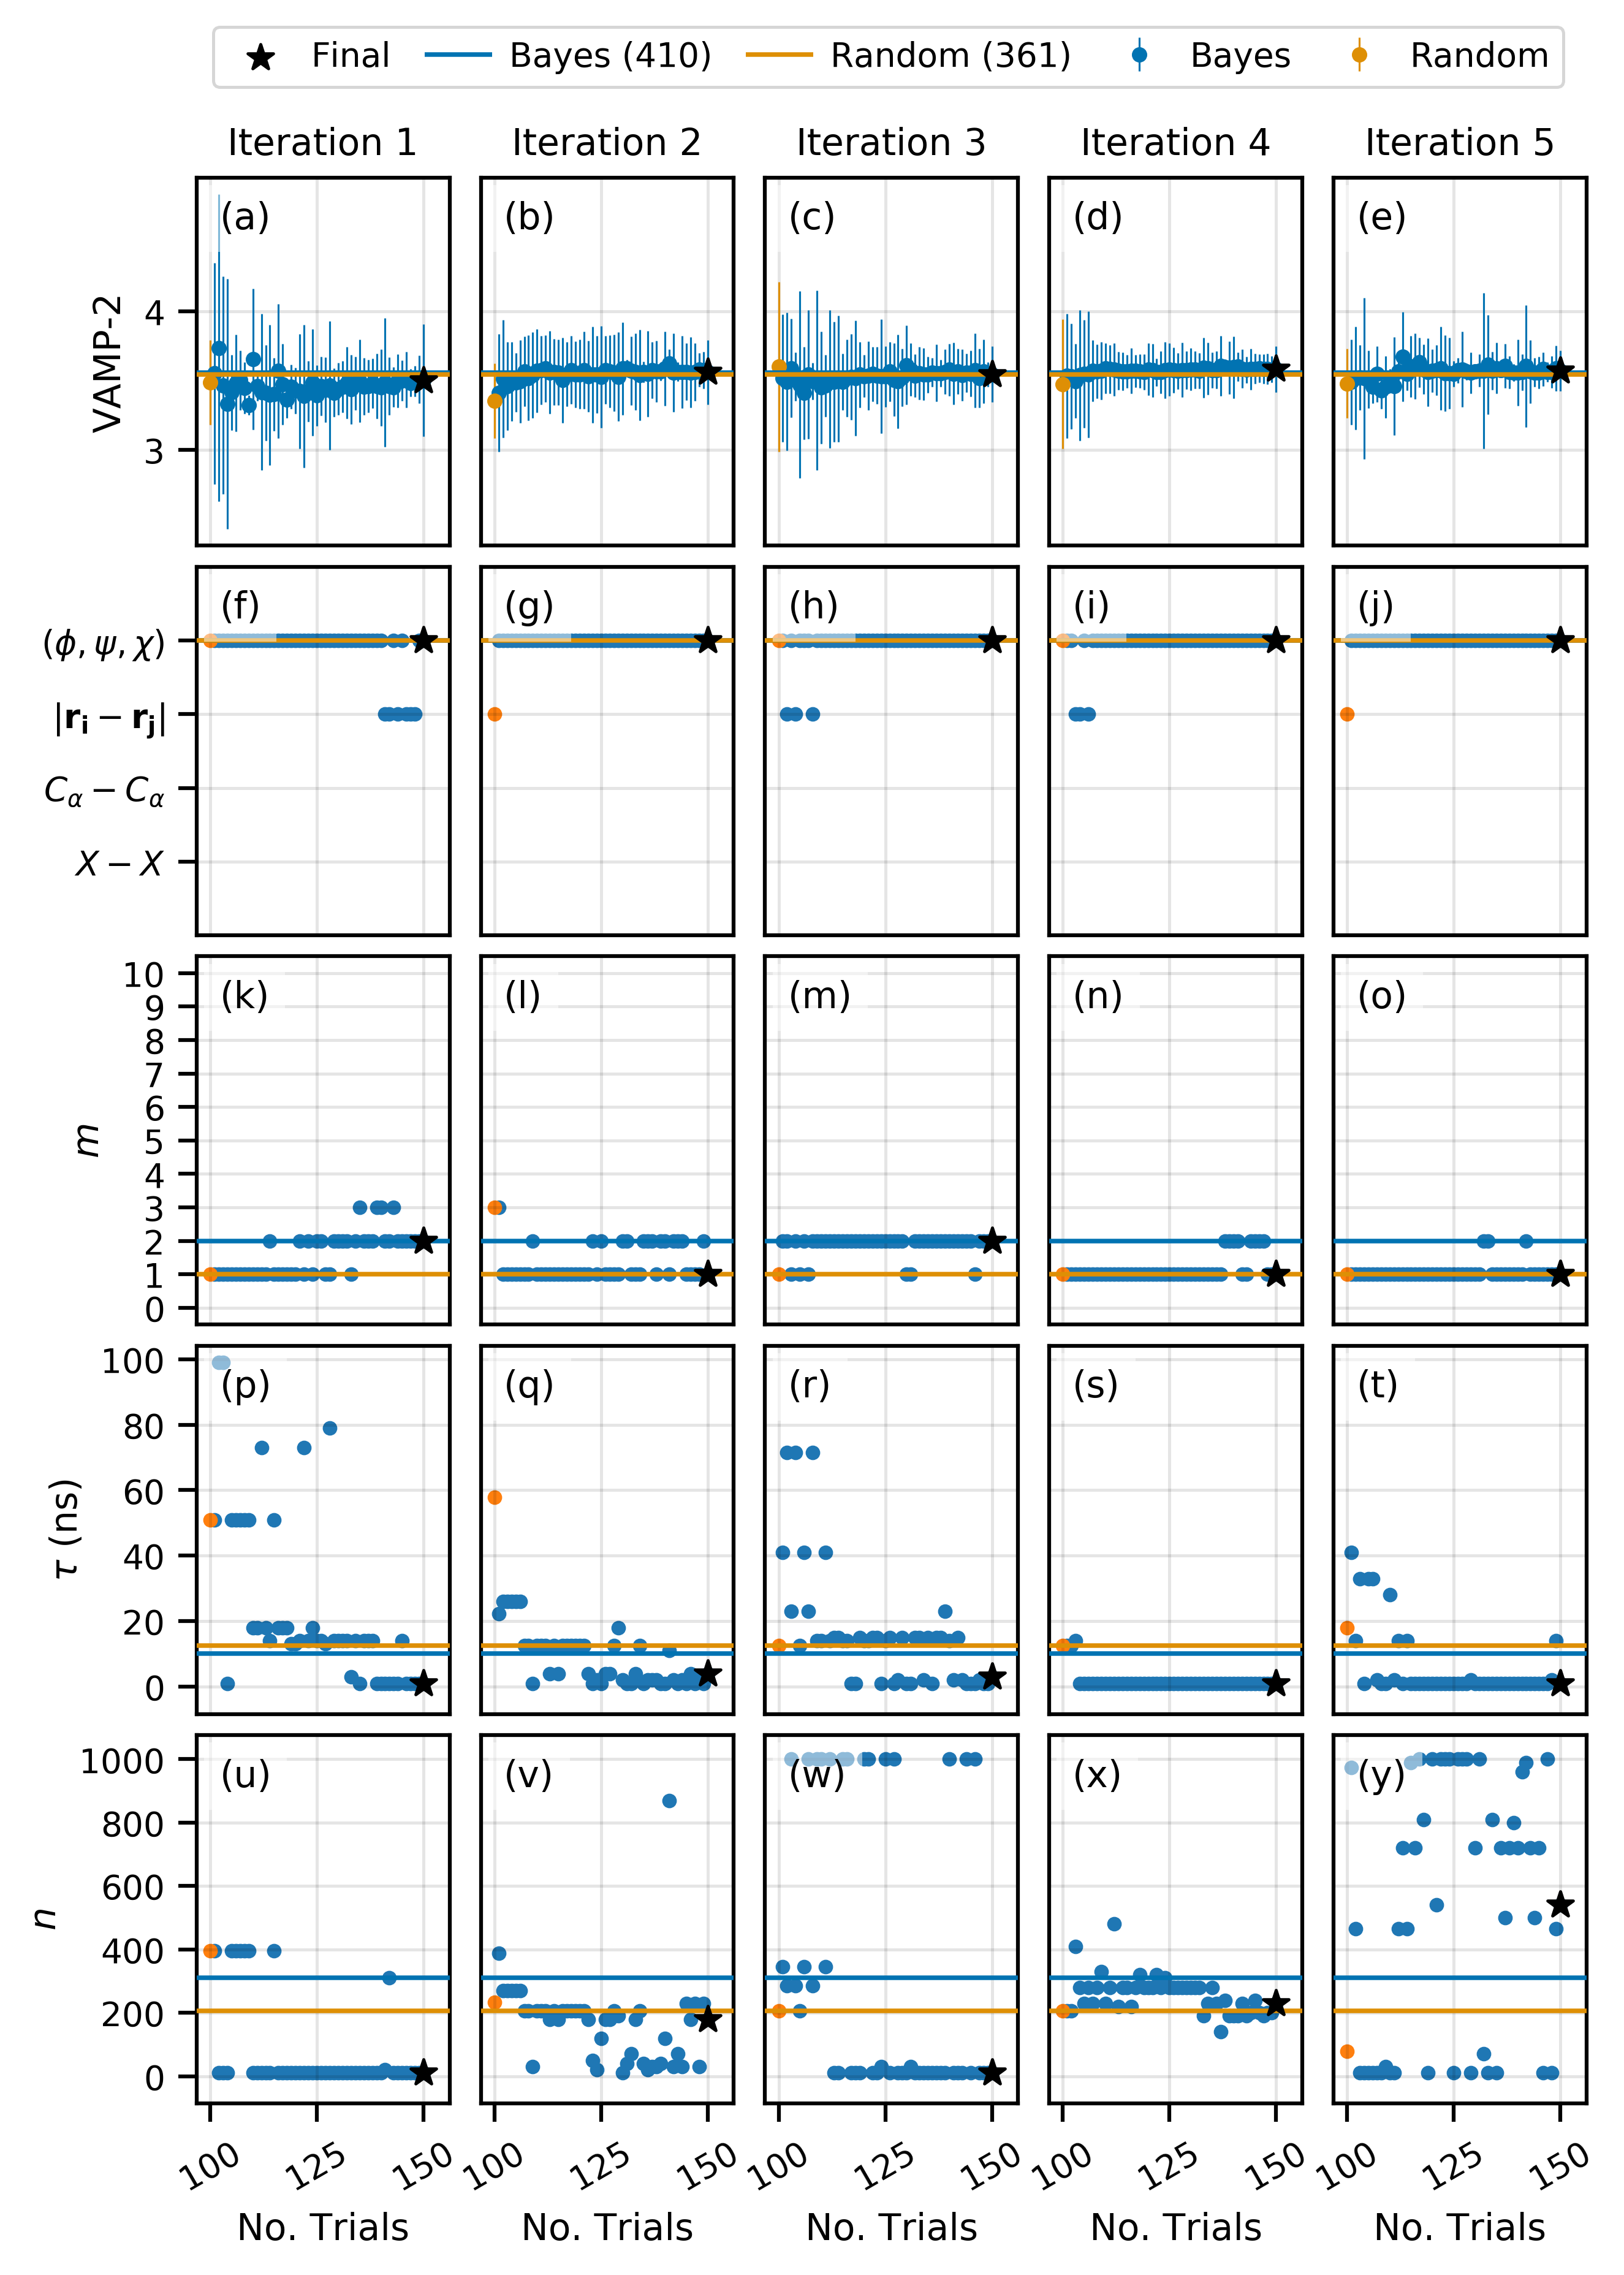
\includegraphics[width=0.8\textwidth]{chapters/msm_optimization/figures/aadh_opt_traj_act_s_d.png}
    
    \label{fig:aadh_opt_traj_d}
\end{figure}

 It is clear from  table \ref{tab:aadh_opt_results} that after Bayesian optimisation each subset had maxima indistinguishable from the maxima of $f(\mathbf{x};\mathcal{D}_{461})$: each had the same optimal feature ($(\phi, \psi, \chi)$ dihedrals), slightly smaller values of $\tau$ ($1 - \SI{4}{\nano\second}$ cf. $\SI{10}{\nano\second}$), similar values of $m$ ($1 - 2$ cf. $2$) but with a range of different values of $n$ ($10 - 540$ cf. $310$). The extent to which these differences to make a difference the final MSM and its interpretation will be discussed in section \ref{subsubsec:sensitivity_analysis} in the context of several sensitivity analyses. 
 
It is also clear that Bayesian optimisation only had a small effect on the value of the incumbent and on the optimum hyper-parameters.  The value of incumbent throughout the procedure (figure \ref{fig:aadh_opt_traj_d} panels (a) - (e)) remain relatively flat. The largest increase came from iteration $4$, with $\Delta \mu 0.108$ and there was even a slight decrease in iteration $3$ with $\Delta \mu = -0.054$. The optimisation procedure also had negligible effects on the value of $\chi$, $m$ and $n$. It did however explore large values of  $\tau$ before settling on its final optimum value in most of the iterations.

The maxima and optimum hyper-parameters of the optimized response surfaces $f^{i}(\mathbf{x};\mathcal{D}_{150})$ are almost indistinguishable from $f(\mathbf{x};\mathcal{D}_{461})$. However the optimisation procedure did not strongly affect the optima of $f^{i}(\mathbf{x};\mathcal{D}_{100})$ compared to $f^{i}(\mathbf{x};\mathcal{D}_{150})$. This suggests that the Bayesian optimisation procedure could be seeded with much fewer trials if a GP model of the response surface could be estimated reliably. 

\subsection{Sensitivity analysis}\label{subsubsec:sensitivity_analysis}

\begin{figure}
    \centering
    \mycaption{Implied timescales of the MSM of AADH with optimized hyper-parameters, estimated using MCMC with 500 posterior draws. Panel (a) shows the implied timescales for $0.1 < \tau(\mathrm{MSM})< \SI{5}{\nano\second}$ and panel (b) for $1 < \tau(\mathrm{MSM}) <\SI{50}{\nano\second}$. The solid lines are the mean of the posteriors, the coloured shaded areas are the  $\SI{95}{\percent}$ credible intervals. The grey shaded area is the region for which the implied timescales are smaller than $\tau(\mathrm{MSM})$.}\label{fig:aadh_its}
    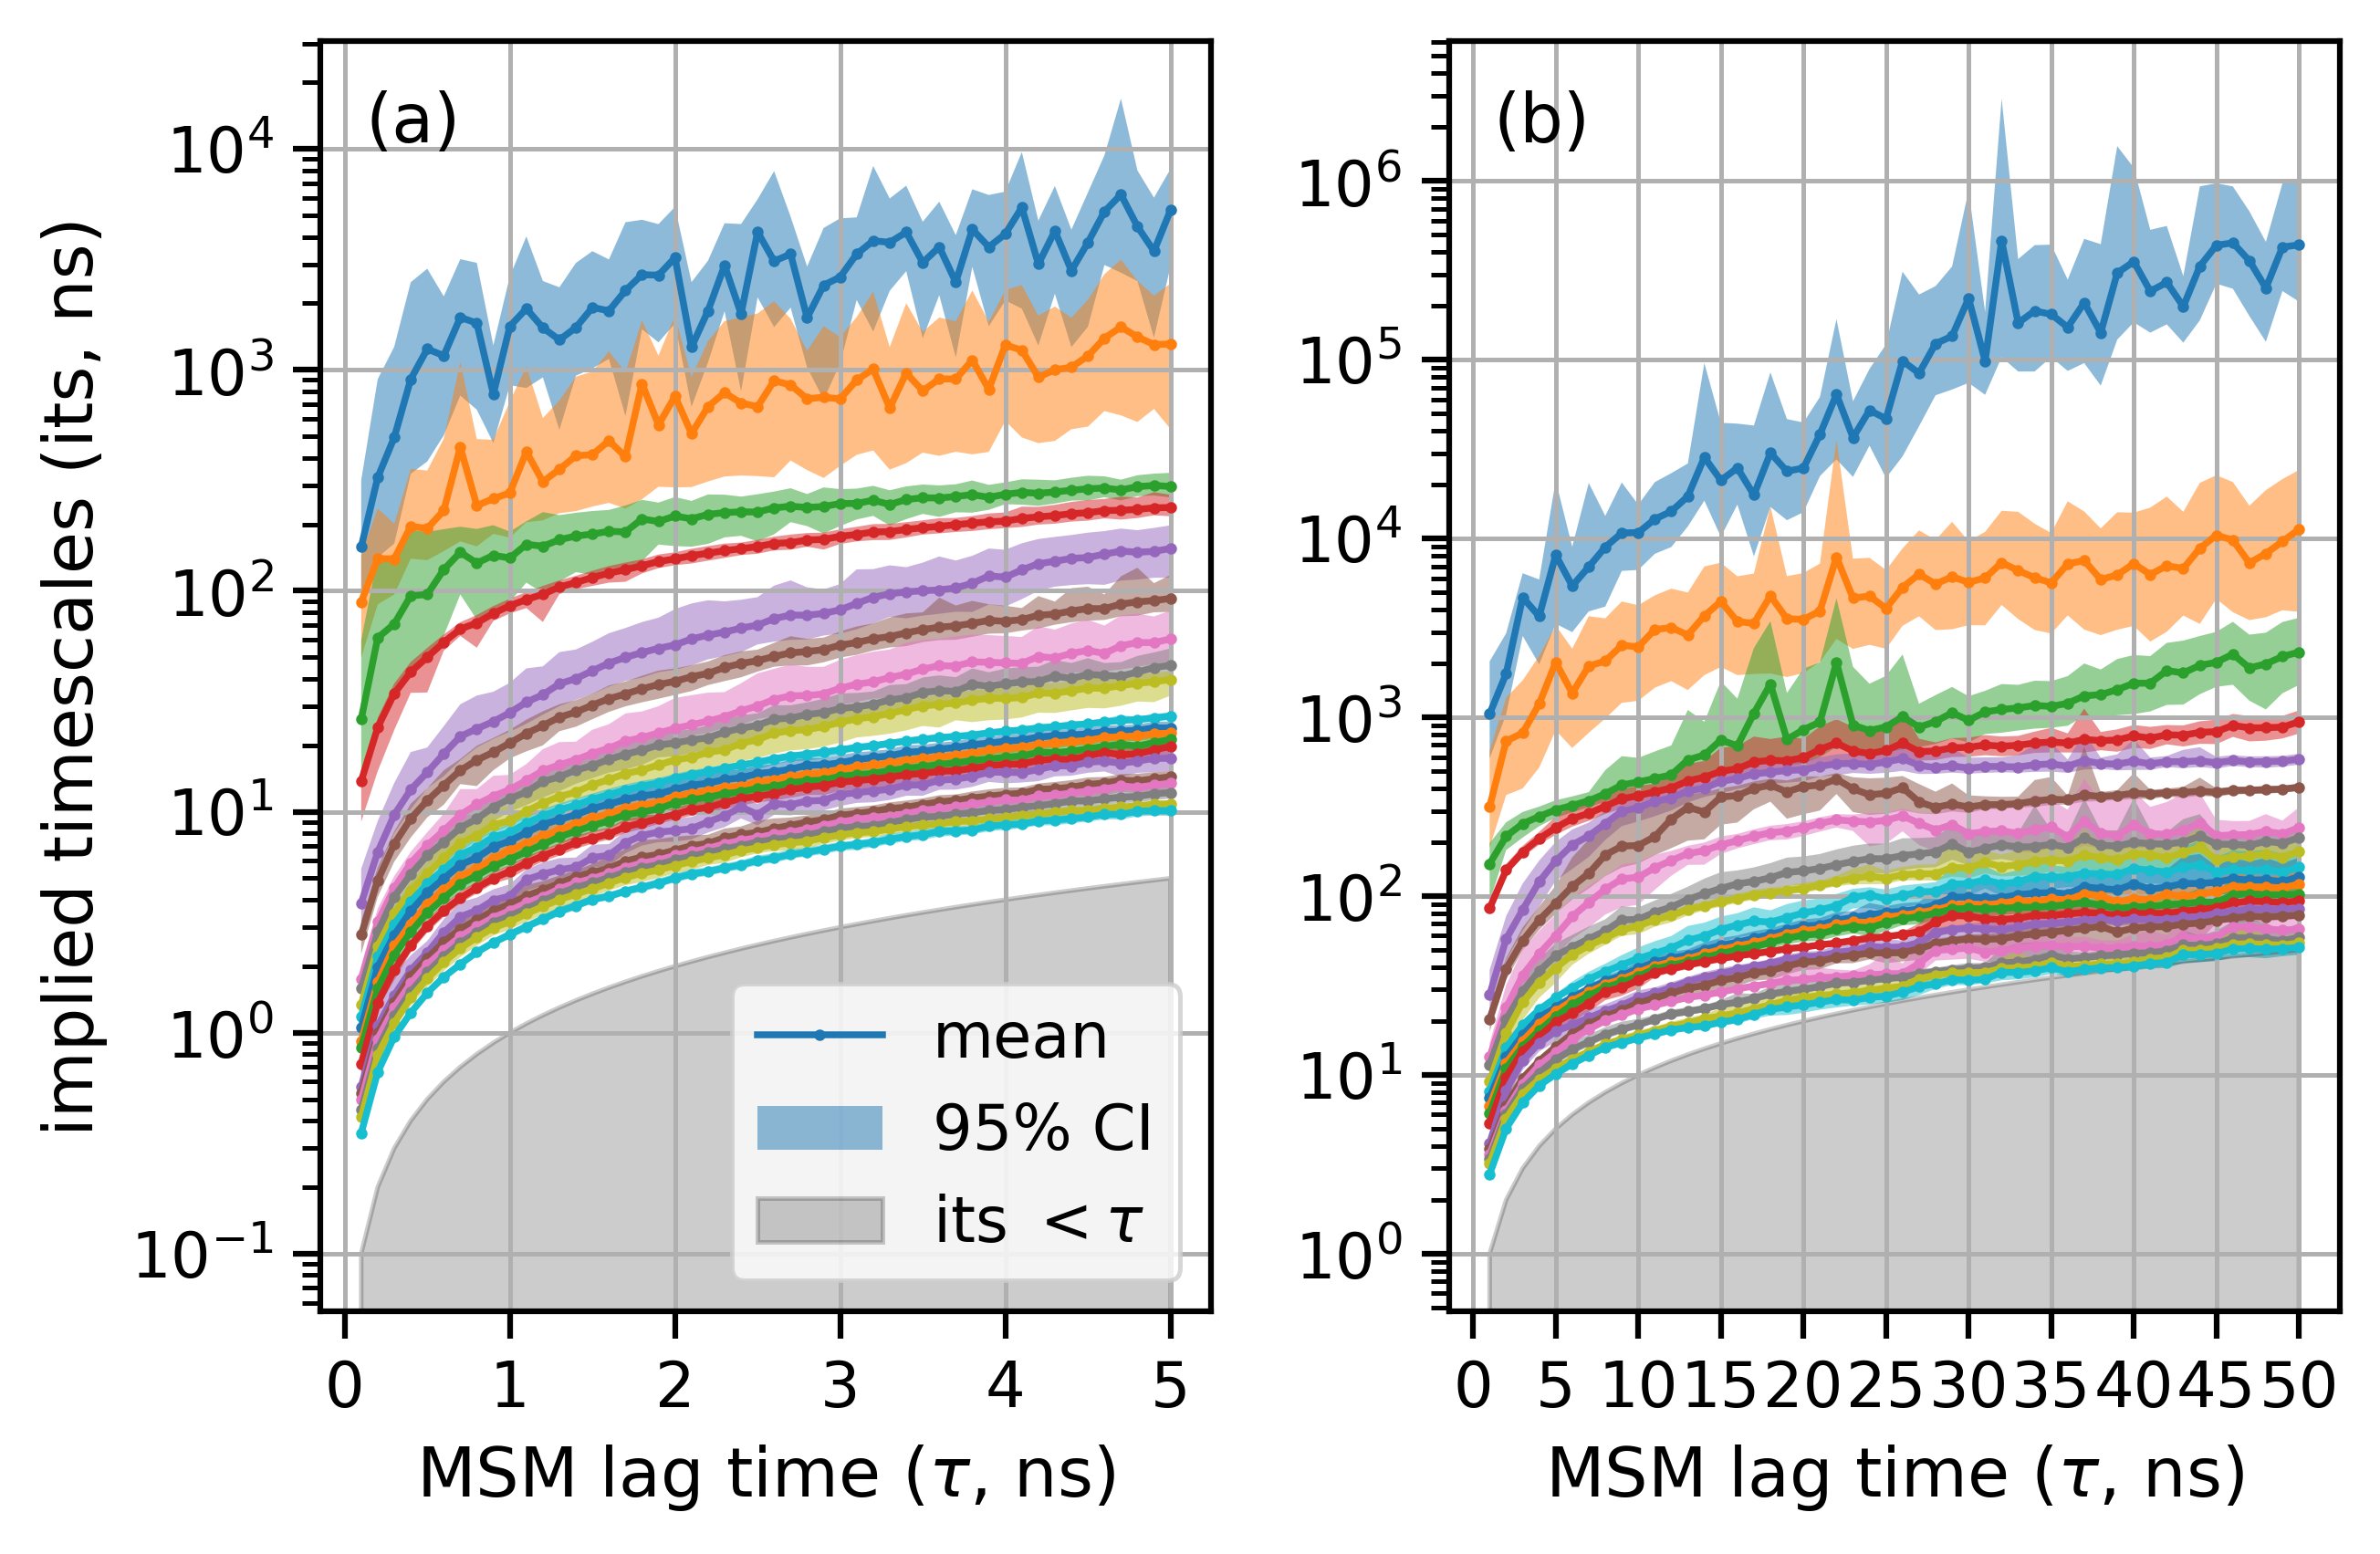
\includegraphics[width=0.9\linewidth]{chapters/msm_optimization/figures/aadh_implied_timescales.png}
\end{figure}

So far the response surface for AADH has been modelled and optimised with a combination of random hyper-parameter sampling and Bayesian optimisation under two assumptions about the model specification: that $\tau(\mathrm{MSM}) = \SI{2}{\nano\second}$ and $k=4$, the number of eigenvalues in the VAMP-2 score, are reasonable assumptions about the lag time and number of slow relaxation processes. As these were established on the basis of the reference MSM it is important to to test these assumptions are still reasonable with the final optimized MSM. 

To test the suitability of $\tau(\mathrm{MSM})$ the eigenvalue spectra of a series of MSMs fit with the optimum hyper-parameters (with $N_{total}=410$, table \ref{tab:aadh_opt_results}) but different lag times are shown in figure \ref{fig:aadh_its}. Panel (a) shows shows lags of  $\SI{0.1}{\nano\second} < \tau(\mathrm{MSM}) < \SI{5}{\nano\second}$ which clearly shows there is a slight increase in the top two implied timescales ($t_{2}$ and $t_{3}$\footnote{I'm using the convention that $t_{1} = \infty$, whose associated eigenvector is the stationary distribution}), suggesting that $\tau^{MSM}$ may be too small. Looking at the implied timescales on a longer timescale $1 < \tau^{MSM} < \SI{50}{\nano\second}$ (panel (b)) shows that there is a small plateau in $t_{2}$ and $t_{3}$  around  $\SIrange{15}{20}{\nano\second}$. It is therefore not possible on this evidence alone to say definitively whether $\tau(\mathrm{MSM})$ should be $2$ or $\SI{20}{\nano\second}$ or whether it makes a difference to non-quantitative aspects of the final model.  

At $\tau = \SI{2}{\nano\second}$ there is no clear separation of timescales between the first four relaxation processes (taking into account the uncertainty in $t_{2}$ and $t_{3}$), however there is a gap between $t_{5}$ and $t_{6}$ suggesting $k=5$ would be more appropriate. This means the fourth relaxation process ($t_{5}$, shown in red in figure \ref{fig:aadh_its}) has not been factored into the response. In principle this means that there may be different hyper-parameters which maximize $\operatorname{VAMP}-2(k=5)$,  given the similarity in $t_{4}$ and $t_{5}$ this may not be very plausible or significant if true. At $\tau = \SI{20}{\nano\second}$ there is a clear separation between $t_{2}$ and $t_{3}$ suggesting $k=2$ is appropriate. In this case we have included potentially too many fast processes. While changing the value of $k$ will certainly change the value of the optimal hyper-parameters, given the mixed evidence in the eigenvalue spectrum there is no reason to reject this optimized MSM. The associated question of how many metastable states and dominant relaxation processes actually matter for explaining the observed data will be investigated further in chapter \ref{chap:hmm}. 

Knowledge of the response surface and of the eigenvalue spectrum suggests sensitivity analyses to understand the validity and robustness of the optimum MSM.  The goal of sensitivity analyses is to have faith that reasonable changes in model choices and hyper-parameters do not materially affect inferences from the model. Typically we are concerned with inferring relaxation timescales ($t_{i}$), the character of the relaxation process ($\Psi_{i}$) and the lumping of the microstates into metastable states. The VAMP-2 score has served as a proxy for the quality of the inferences required from the model but this is not sufficient  for a number of reasons.  First, as discussed above it will be sensitive to both the MSM lag time and the number of eigenfunctions used in the definition. Second, as figure \ref{fig:ala1_evcompare} has demonstrated, VAMP-2 is not sensitive to the discretisation error. This is also evident in the fact that in both iteration $1$ and $3$ (table \ref{tab:aadh_opt_results}) the optimal value of $n=10$ with only a very small difference in response at these values $\mu = 3.500$ and   $\mu=3.545$ cf. $\mu=3.558$). Third, the phenomenon of the Rashomon effect \cite{breiman2001} in statistical modelling, where  multiple \emph{different} statistical models result in the performance metric, could be at play here.

The standard validation check of MSMs, the Chapman-Kolmogorov test (equation \ref{eqn:ck_test}), relies on coarse graining transition matrix, which will be discussed in detail in chapter \ref{chap:hmm}. The current discussion will center on the eigenvalue spectrum and qualitative aspects of the free energy surface and eigenfunctions. For the optimal MSM, these are all shown in figure \ref{fig:aadh_msm_best}: panels (a) - (c) show the normalised eigenvectors of the first three relaxation processes ($\Psi_{2} - \Psi_{3}$) in the space of the first two TICA components. A coarse grained color map has been applied to make the sign structure, rather than the absolute value of eigenvector, more apparent: $|\Psi_{2}| < 1e^{-2}$ are coloured white, $\Psi_{2}> 0$ red,  and $\Psi_{2} < 0$ blue. Panel (d) shows the implied timescales for the first $10$ relaxation processes (coloured according to whether they were included in the $\operatorname{VAMP-2}$ score), and panel (e) shows the free energy surface in the space of the first two TICA components. 

\begin{figure}
    \centering
    \mycaption{The final, optimised response surface of AADH fit using the $361$ randomly sampled hyper-parameter trials and the $50$ trials selected in the Bayesian optimisation procedure. For each feature a single heat map are shown for $n=310$, with $\tau$ on the vertical axis and $m$ on the horizontal axis. All values of $m$ in the range $1\le m \le 10$ are shown. The white star denotes the approximate location of the maximum of the surface, the true maximum occurs at $\tau=\SI{10}{\nano\second}, m=2, n=310$. The value of the response surface denoted by the color (lighter implied higher values) and with the text annotations. }
    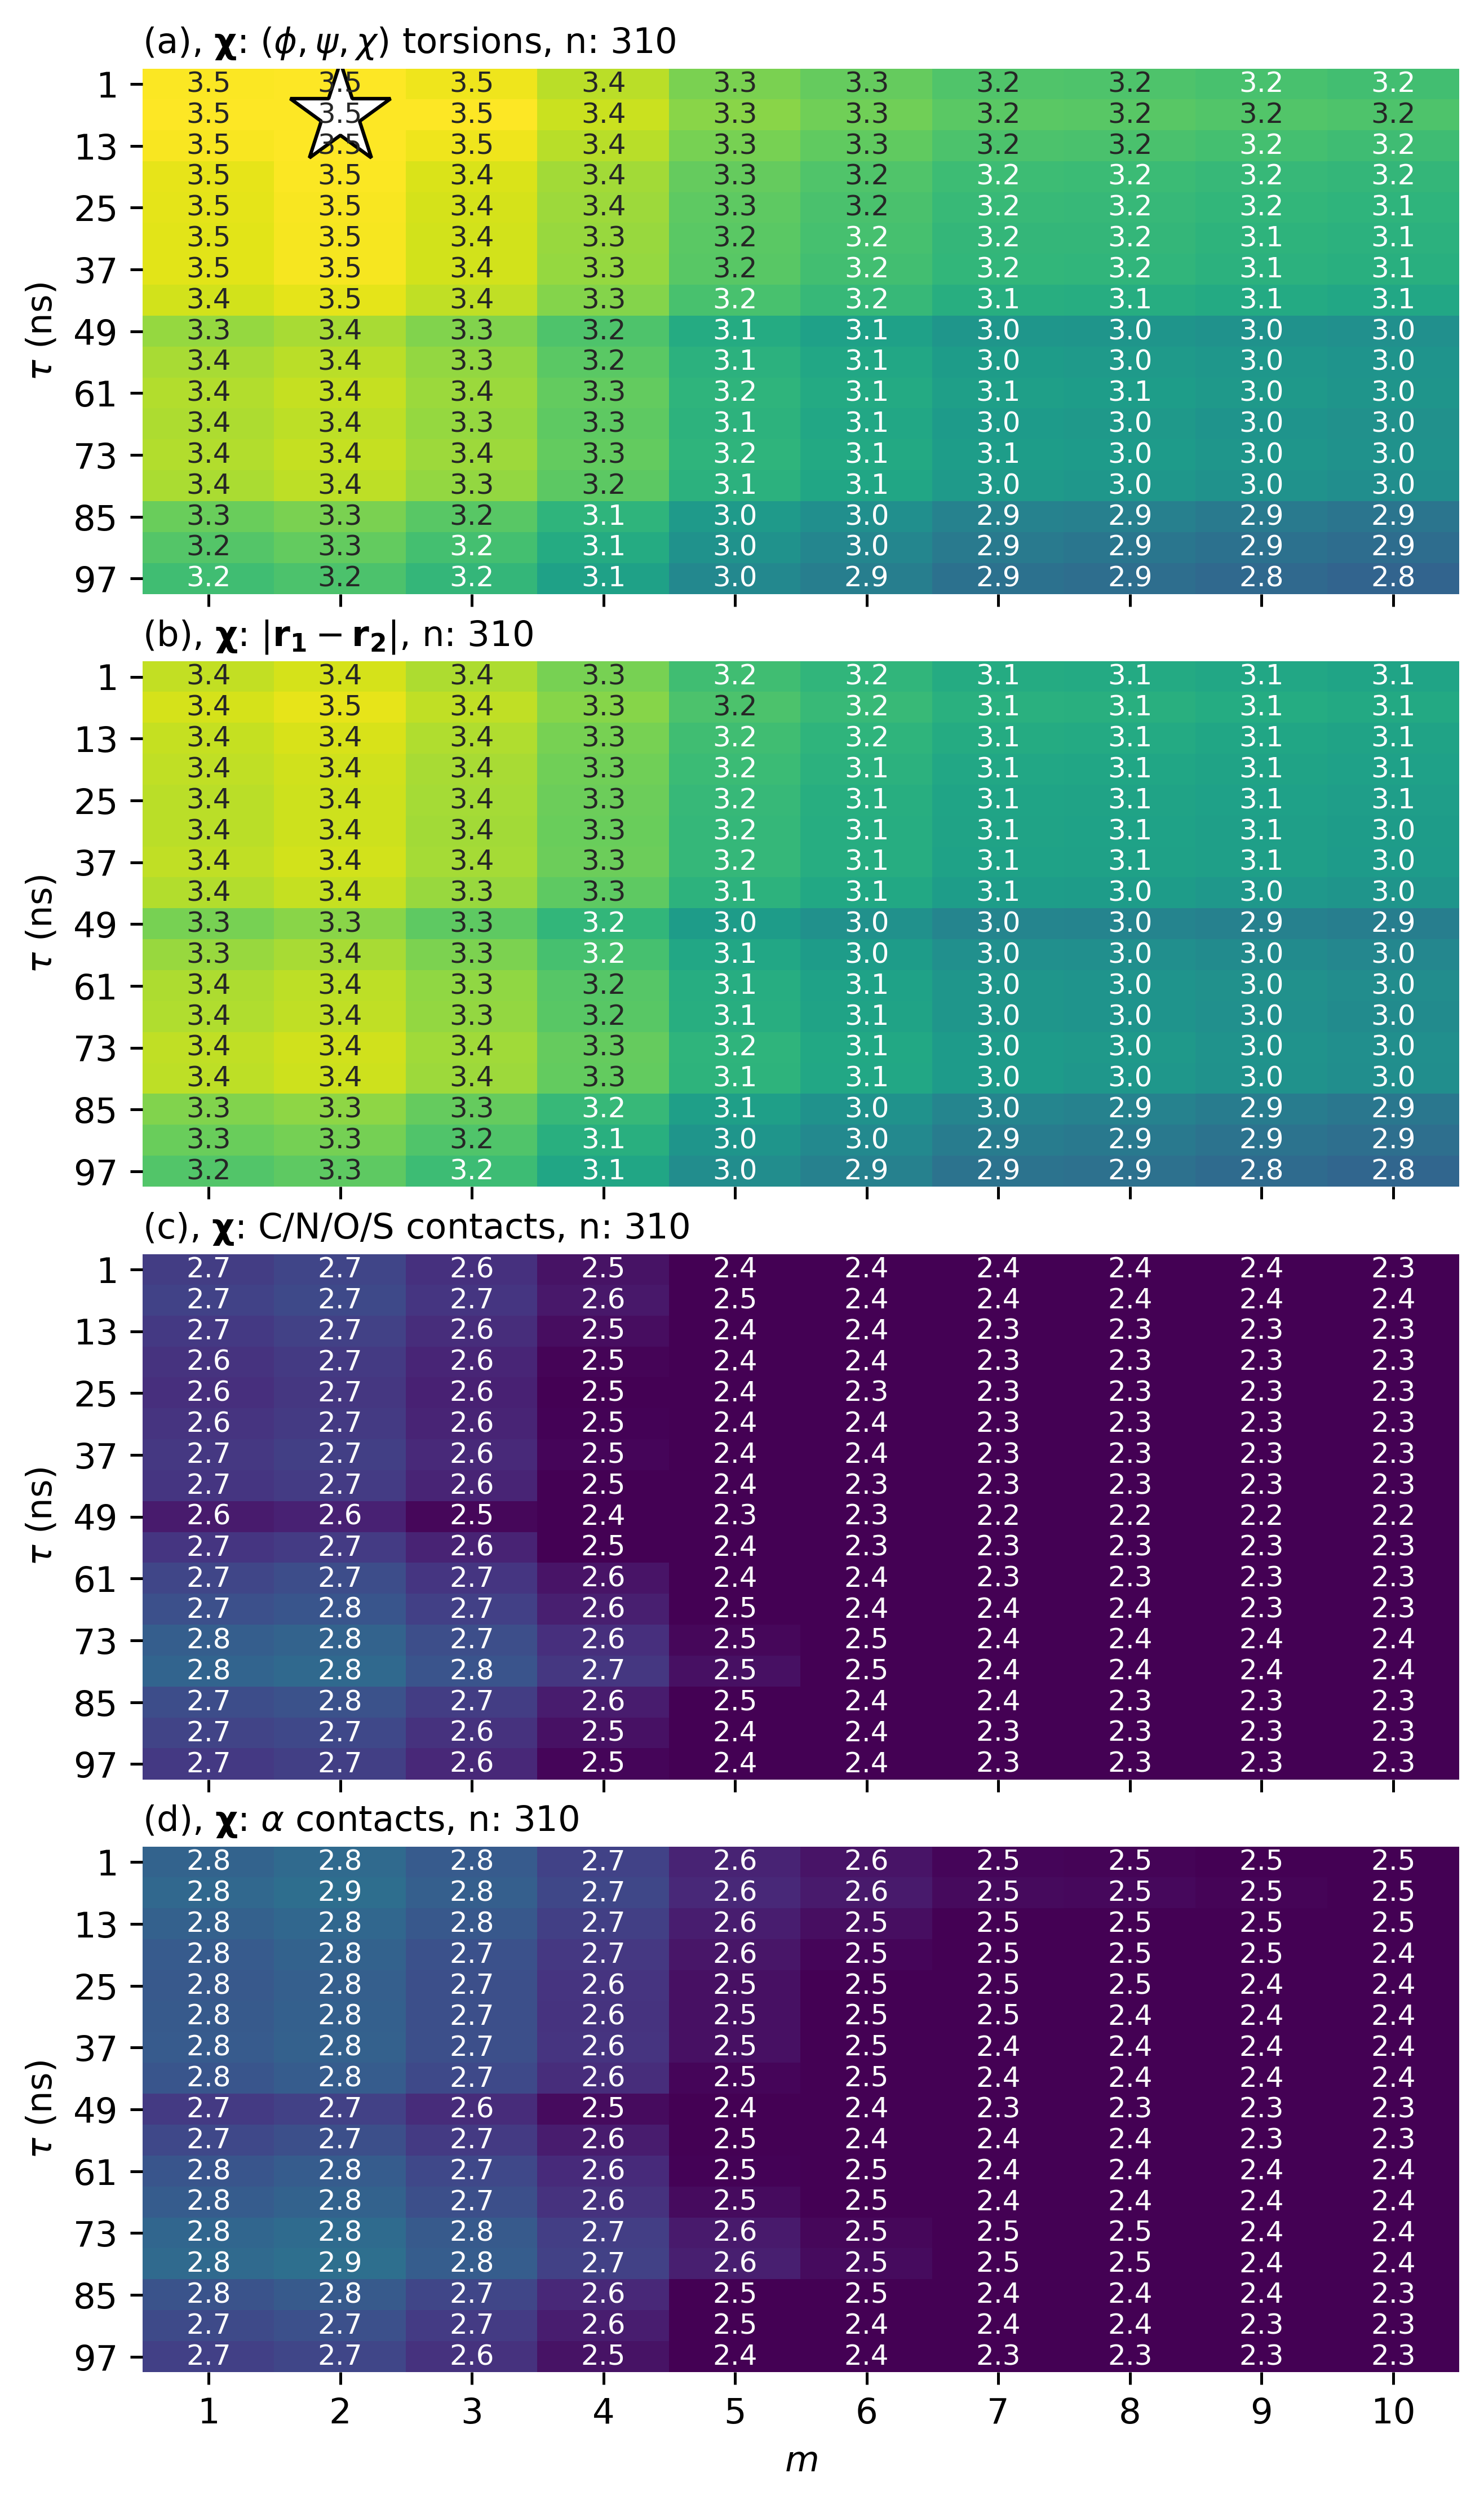
\includegraphics[width=0.6\textwidth]{chapters/msm_optimization/figures/aadh_response_surface_d_opt.png.png}
    \label{fig:aadh_rsm_opt}
\end{figure}


\begin{figure}
    \centering
    \mycaption{[TM: label axes] MSM of AADH with optimum hyper-parameters: $\chi= (\phi, \psi, \chi)$ torsions, $\tau=\SI{10}{\nano\second}$, $m=2$ and $n=310$. Panels (a), (b) and (c) show the non-trivial eigenvectors used in the VAMP-2 score, the horizontal and vertical axes are the first two TICA components. Panel (d) are the first ten implied timescales, colored according to whether they were used in the VAMP-2 score. The error bars are the $\SI{95}{\percent}$ credible intervals.  Panel (e) is the free energy with the same axes as panels (a) - (c). The MSM was estimated using MCMC with 1000 samples of the posterior.}
    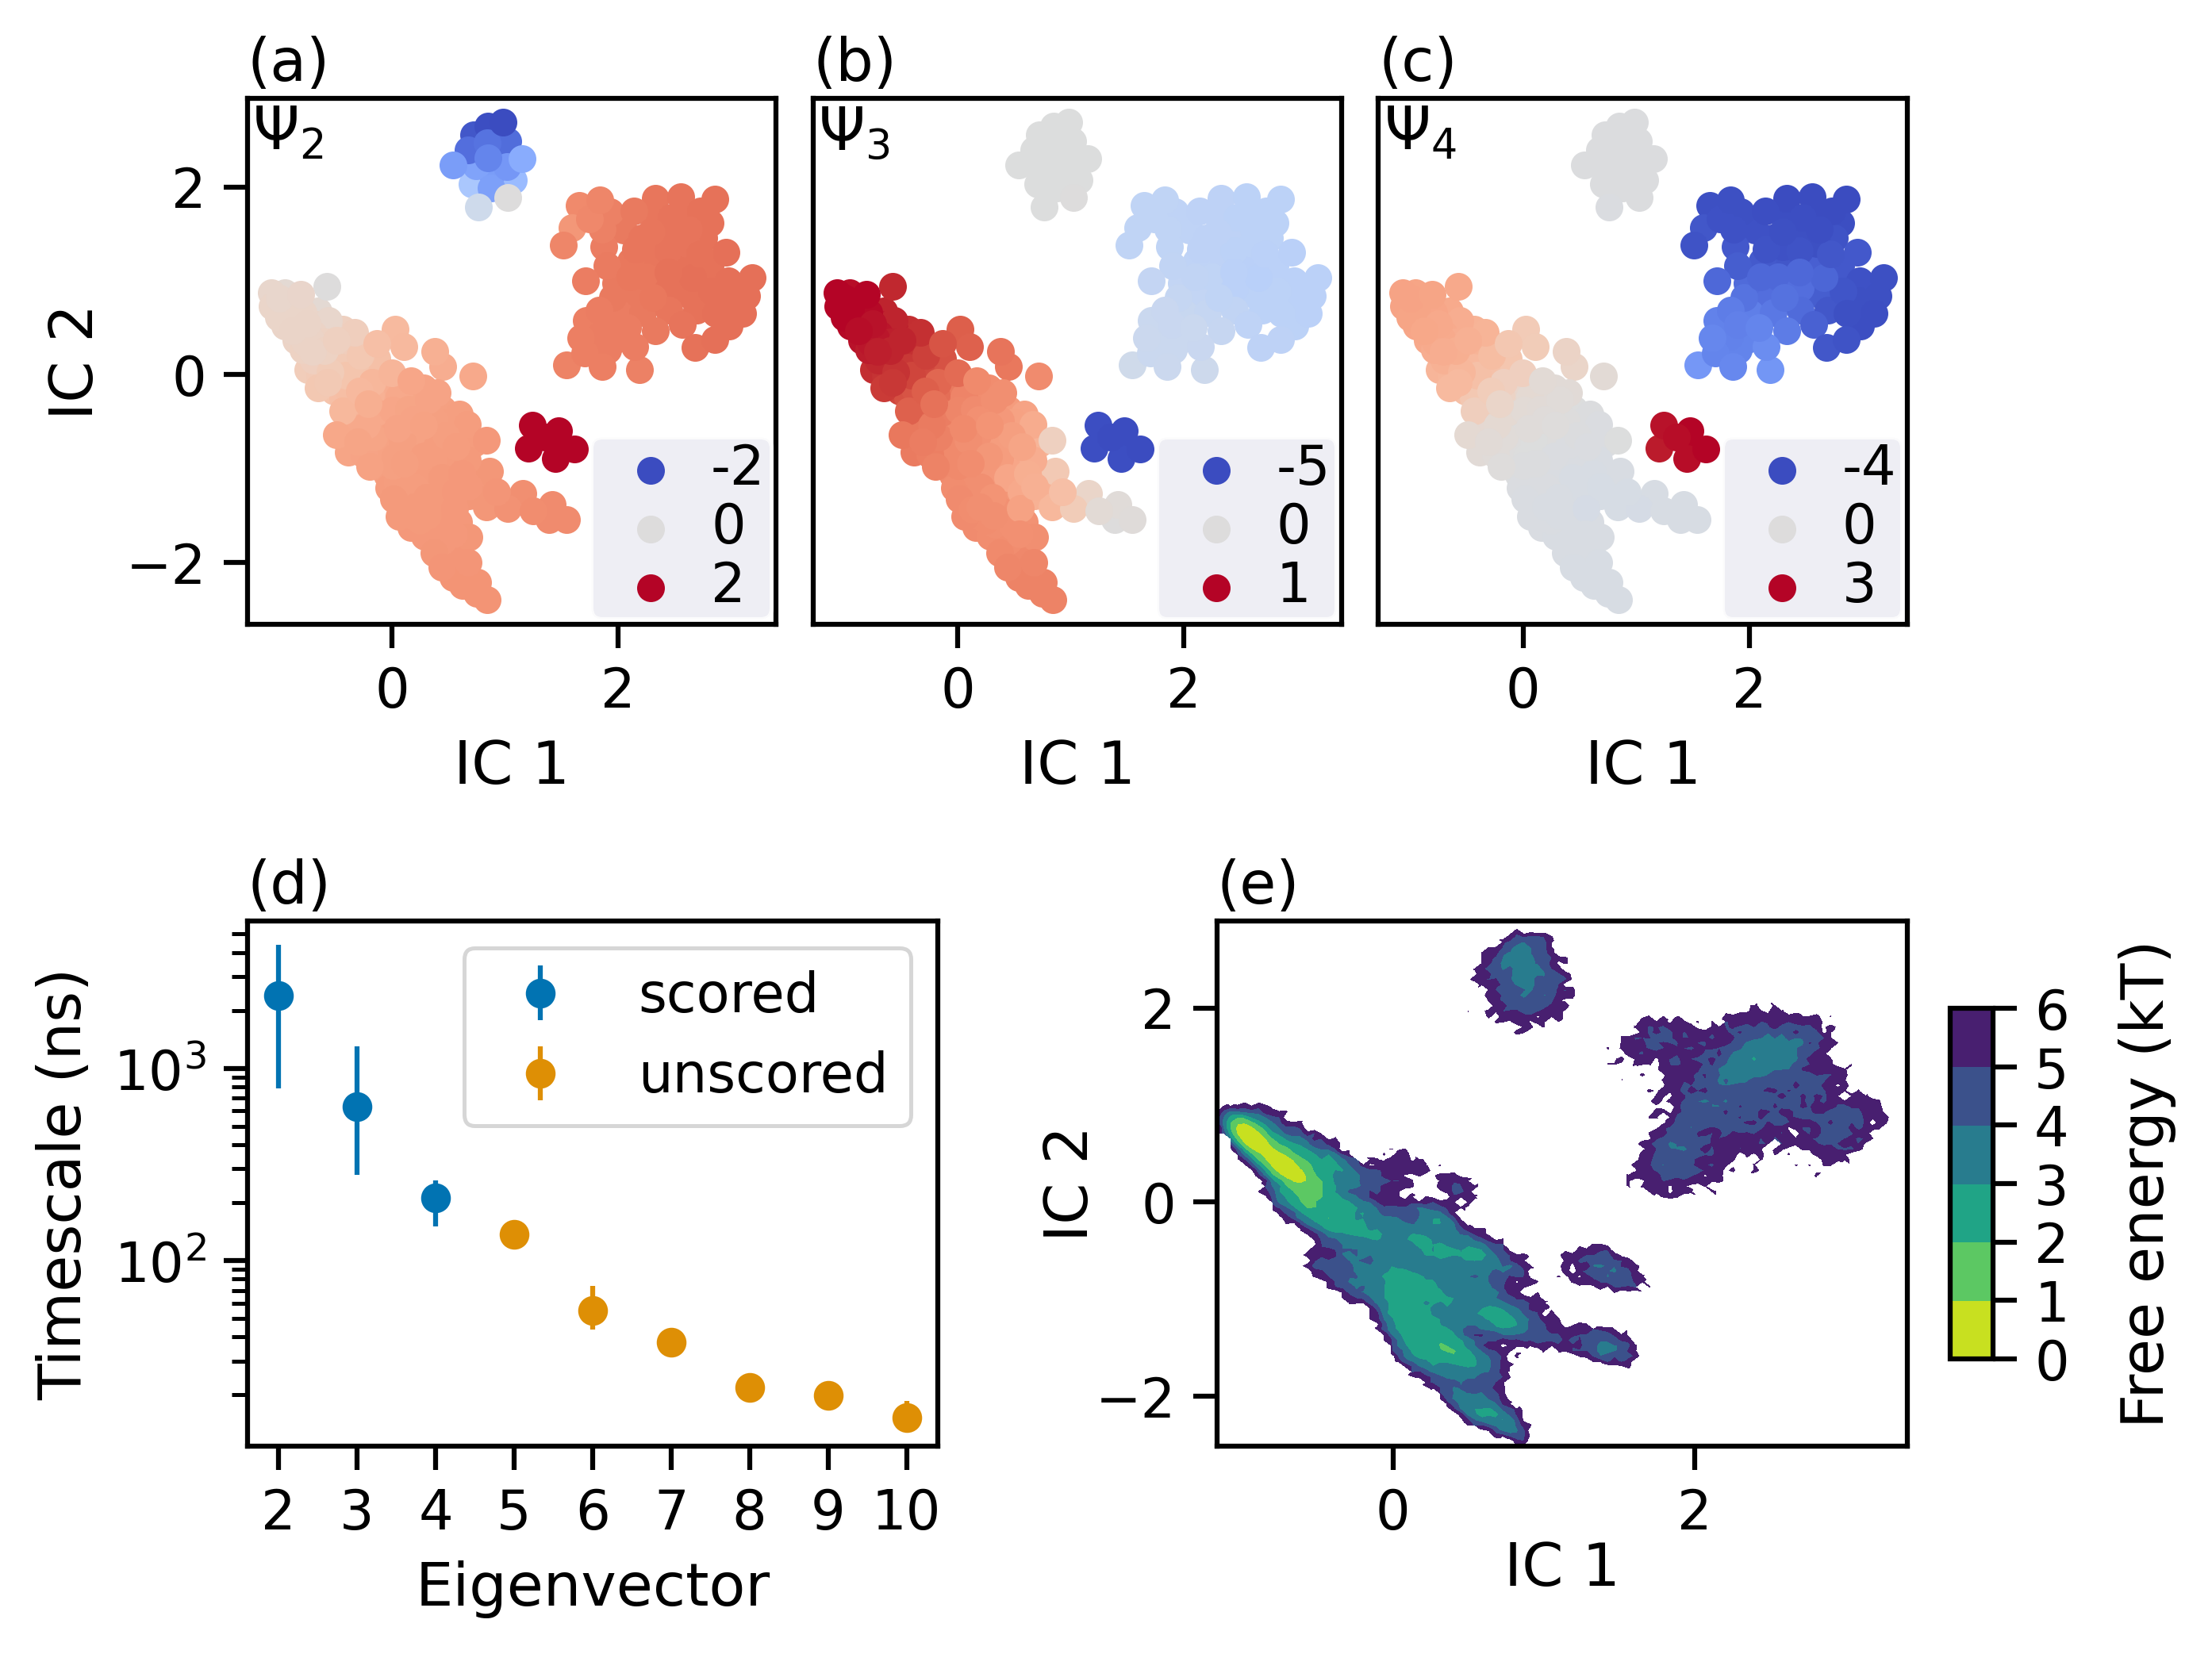
\includegraphics[width=0.7\textwidth]{chapters/msm_optimization/figures/aadh_msm_best.png}
    \label{fig:aadh_msm_best}
\end{figure}

\begin{figure}
    \centering
    \mycaption{Sensitivity 1: MSM of AADH with the same hyper-parameters as the base case  but with $\tau(\mathrm{MSM})=\SI{20}{\nano\second}$. See caption of figure \ref{fig:aadh_msm_best} for details. }
    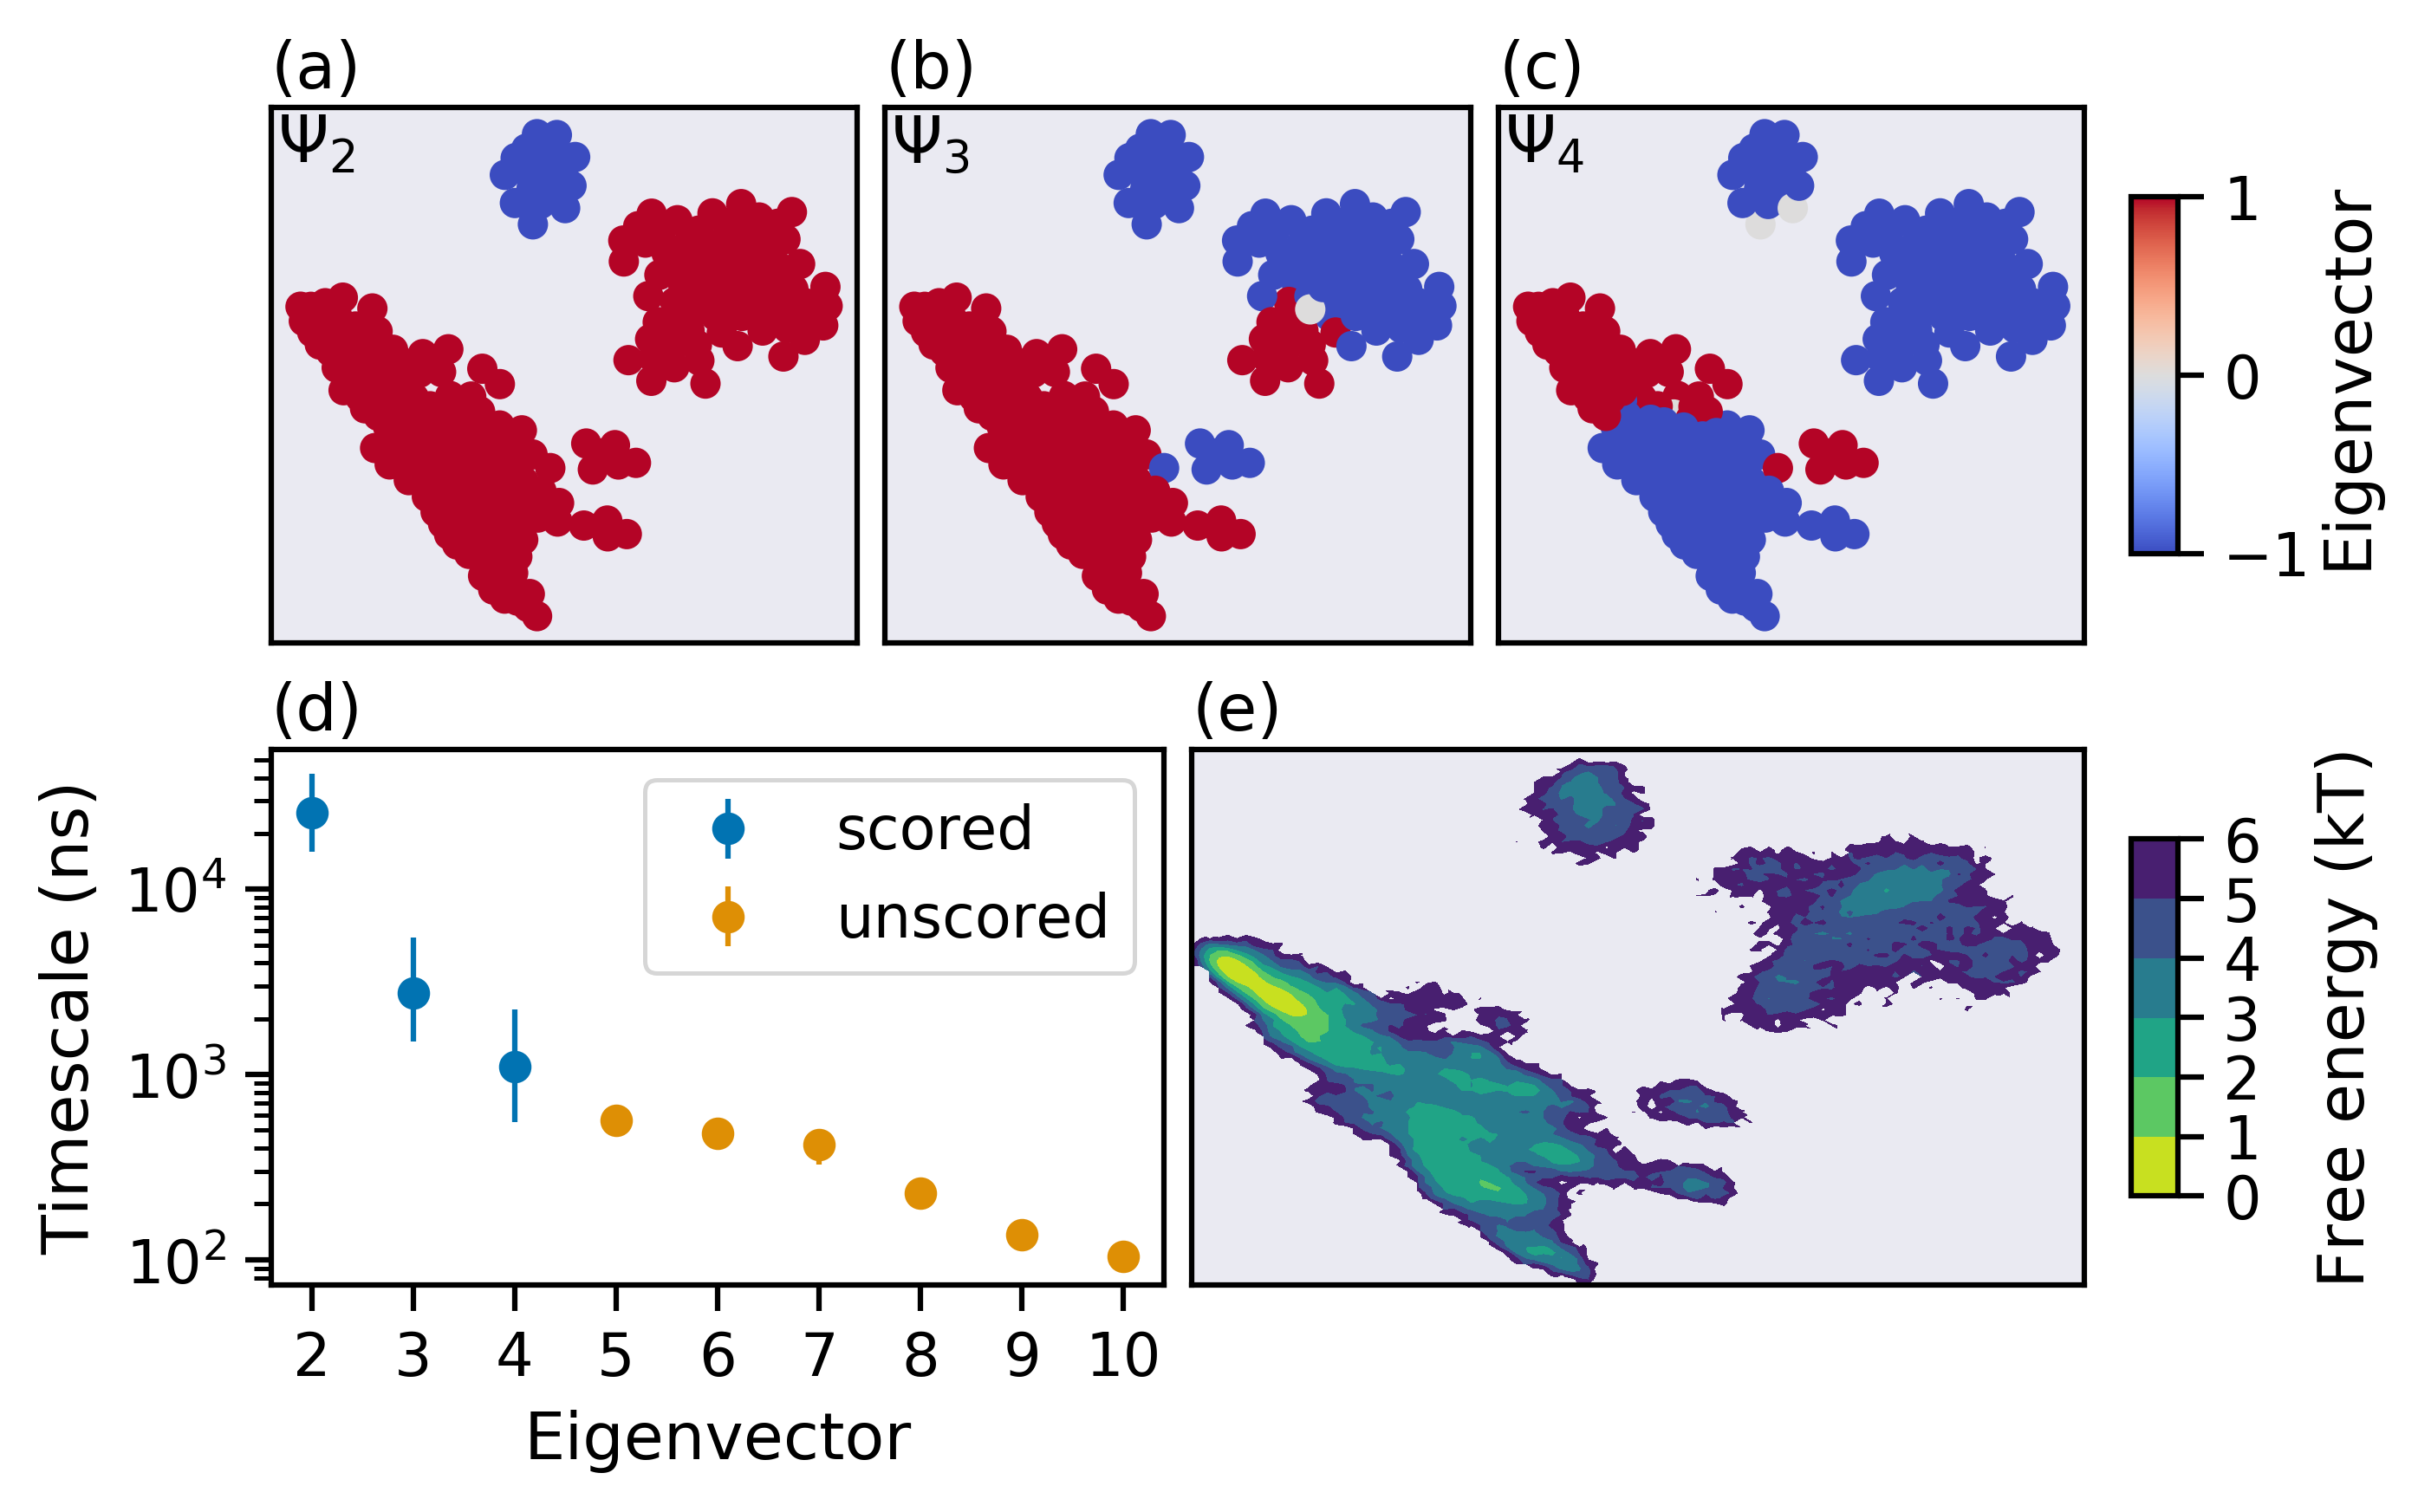
\includegraphics[width=0.7\textwidth]{chapters/msm_optimization/figures/aadh_msm_sens_1.png}
    \label{fig:aadh_msm_sens_1}
\end{figure}

Figure \ref{fig:aadh_msm_best} will serve as a base-case for a number of sensitivity analyses which are informed by the optimised response surface (figure \ref{fig:aadh_rsm_opt}) and eigenvalue spectrum (figure \ref{fig:aadh_its}).

Sensitivity 1 changed the MSM lag time from $\SI{2}{\nano\second}$ to $\SI{20}{\nano\second}$ and is shown in figure \ref{fig:aadh_msm_sens_1}. As expected the absolute values of the implied timescales have increased, as has the relative separation between $t_{2}$/$t_{3}$. The values of relaxation timescales are summarised in table \ref{tab:sens_ts}. The sign structure of the first and third relaxation process remains the same, but for the second and third relaxation process this has changed.  We can conclude that the first, definitely slow, relaxation process is robust with respect to it's sign structure. The second relaxation process which may or may not be dominant, changes its character as a function of the MSM lag time and so  $\tau(\mathrm{MSM}) = \SI{20}{\nano\second}$ will need to be included in the coarse graining analysis in chapter \ref{chap:hmm}. 

\begin{figure}
    \centering
    \caption{Sensitivity 2: MSM of AADH with the best hyper-parameters of with the interatomic distances feature ($\tau = \SI{1}{\nano\second}, m=2, n=110$) and $\tau(\mathrm{MSM}) \SI{2}{\nano\second}$. See caption of figure \ref{fig:aadh_msm_best} for details.}
    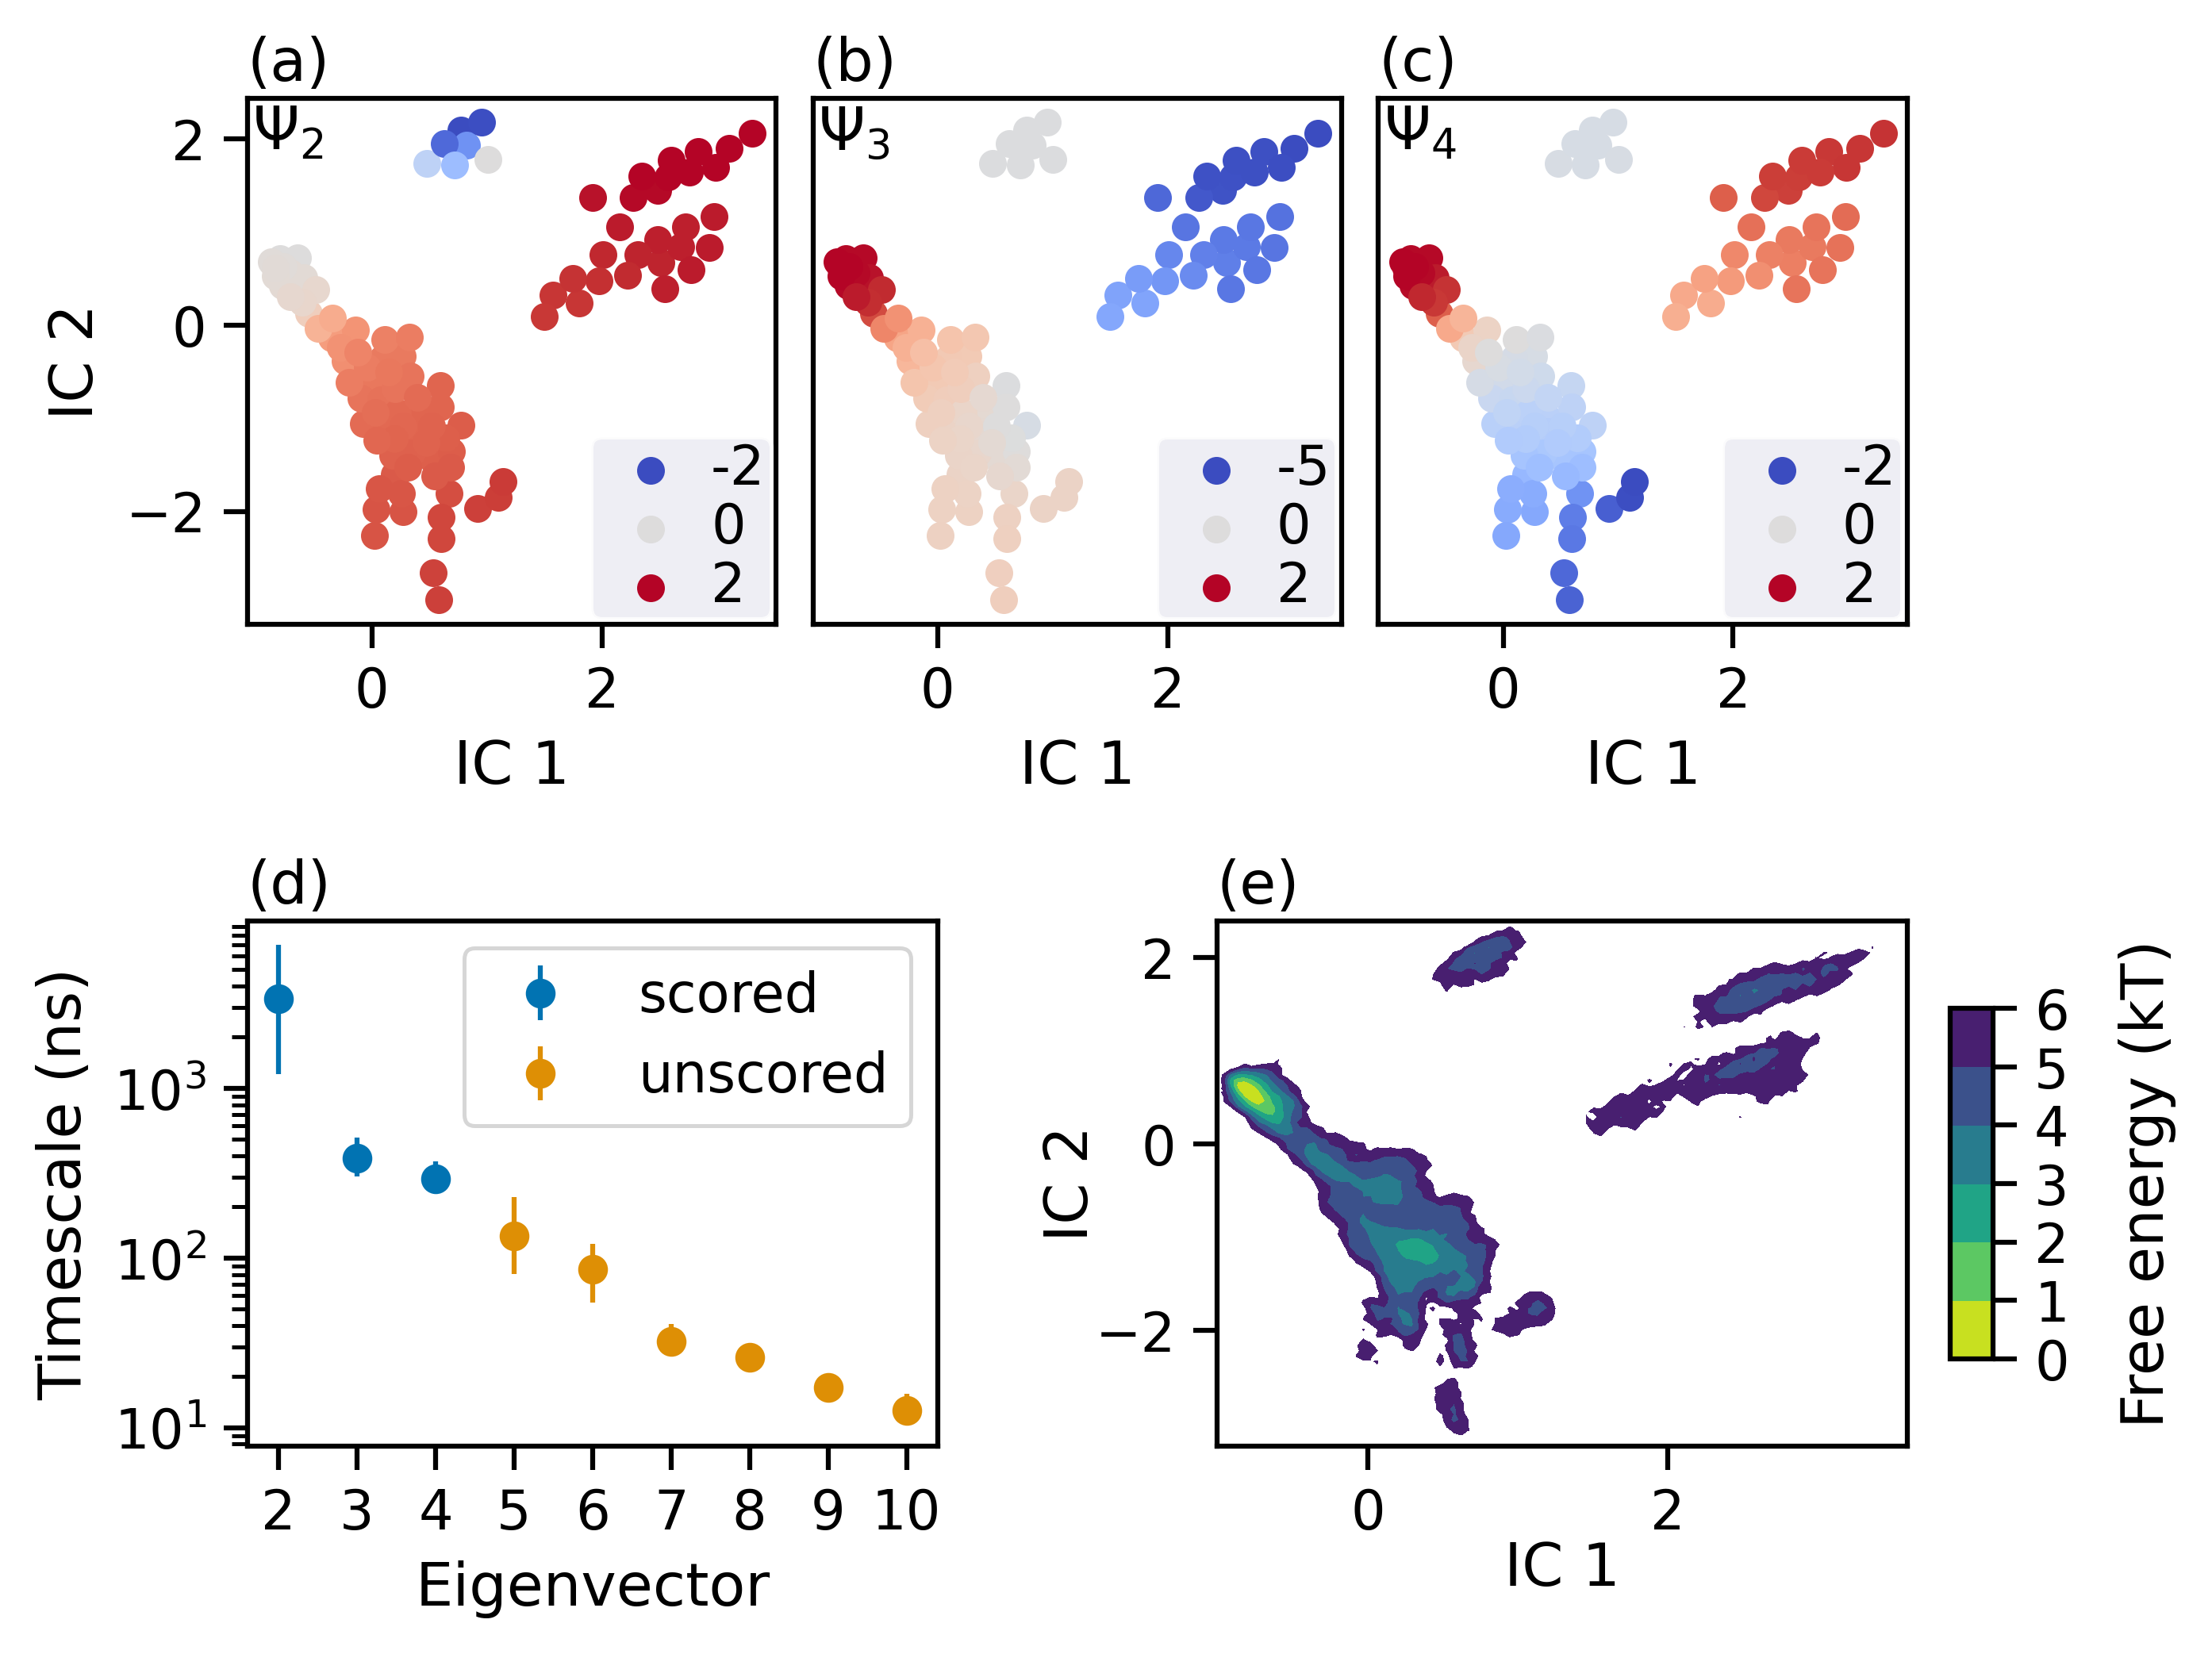
\includegraphics[width=0.8\textwidth]{chapters/msm_optimization/figures/aadh_msm_sens_2.png}
    \label{fig:aadh_msm_sens_2}
\end{figure}


Sensitivity 2 changed the hyper-parameters to the best performing set with the interatomic distances feature ($\tau = \SI{1}{\nano\second}, m=2, n=110$) and is shown in figure \ref{fig:aadh_msm_sens_2}.  This was justified because of the similarity in response values (incumbent: $\mu=3.56 \pm 0.18$, sensitivity 2: $\mu=3.44 \pm 0.35$). There is a clear similarity between sensitivity 2 and the base case in both the free energy surface and the first relaxation processes' timescale ($t_{2} = \SI{2.7}{\micro\second}$ cf.$t_{2} = \SI{2.2}{\micro\second}$ in the base case) and sign structure.  There is also a greater separation in timescales between $t_{2}$ and $t_{3}$ ($t_{2}/t_{3} \simeq 6$) than the base case ($t_{2}/t_{3} \simeq 2$). Taken together these two observations suggest that the interatomic distances resolve the first relaxation processes similarly but not the second relaxation process. 


\begin{figure}
    \centering
    \caption{Sensitivity 3: MSM of AADH with the same hyper-parameters of the MSM as the base case but a long TICA lag time $\tau = \SI{85}{\nano\second}$.  See caption of figure \ref{fig:aadh_msm_best} for details.}
    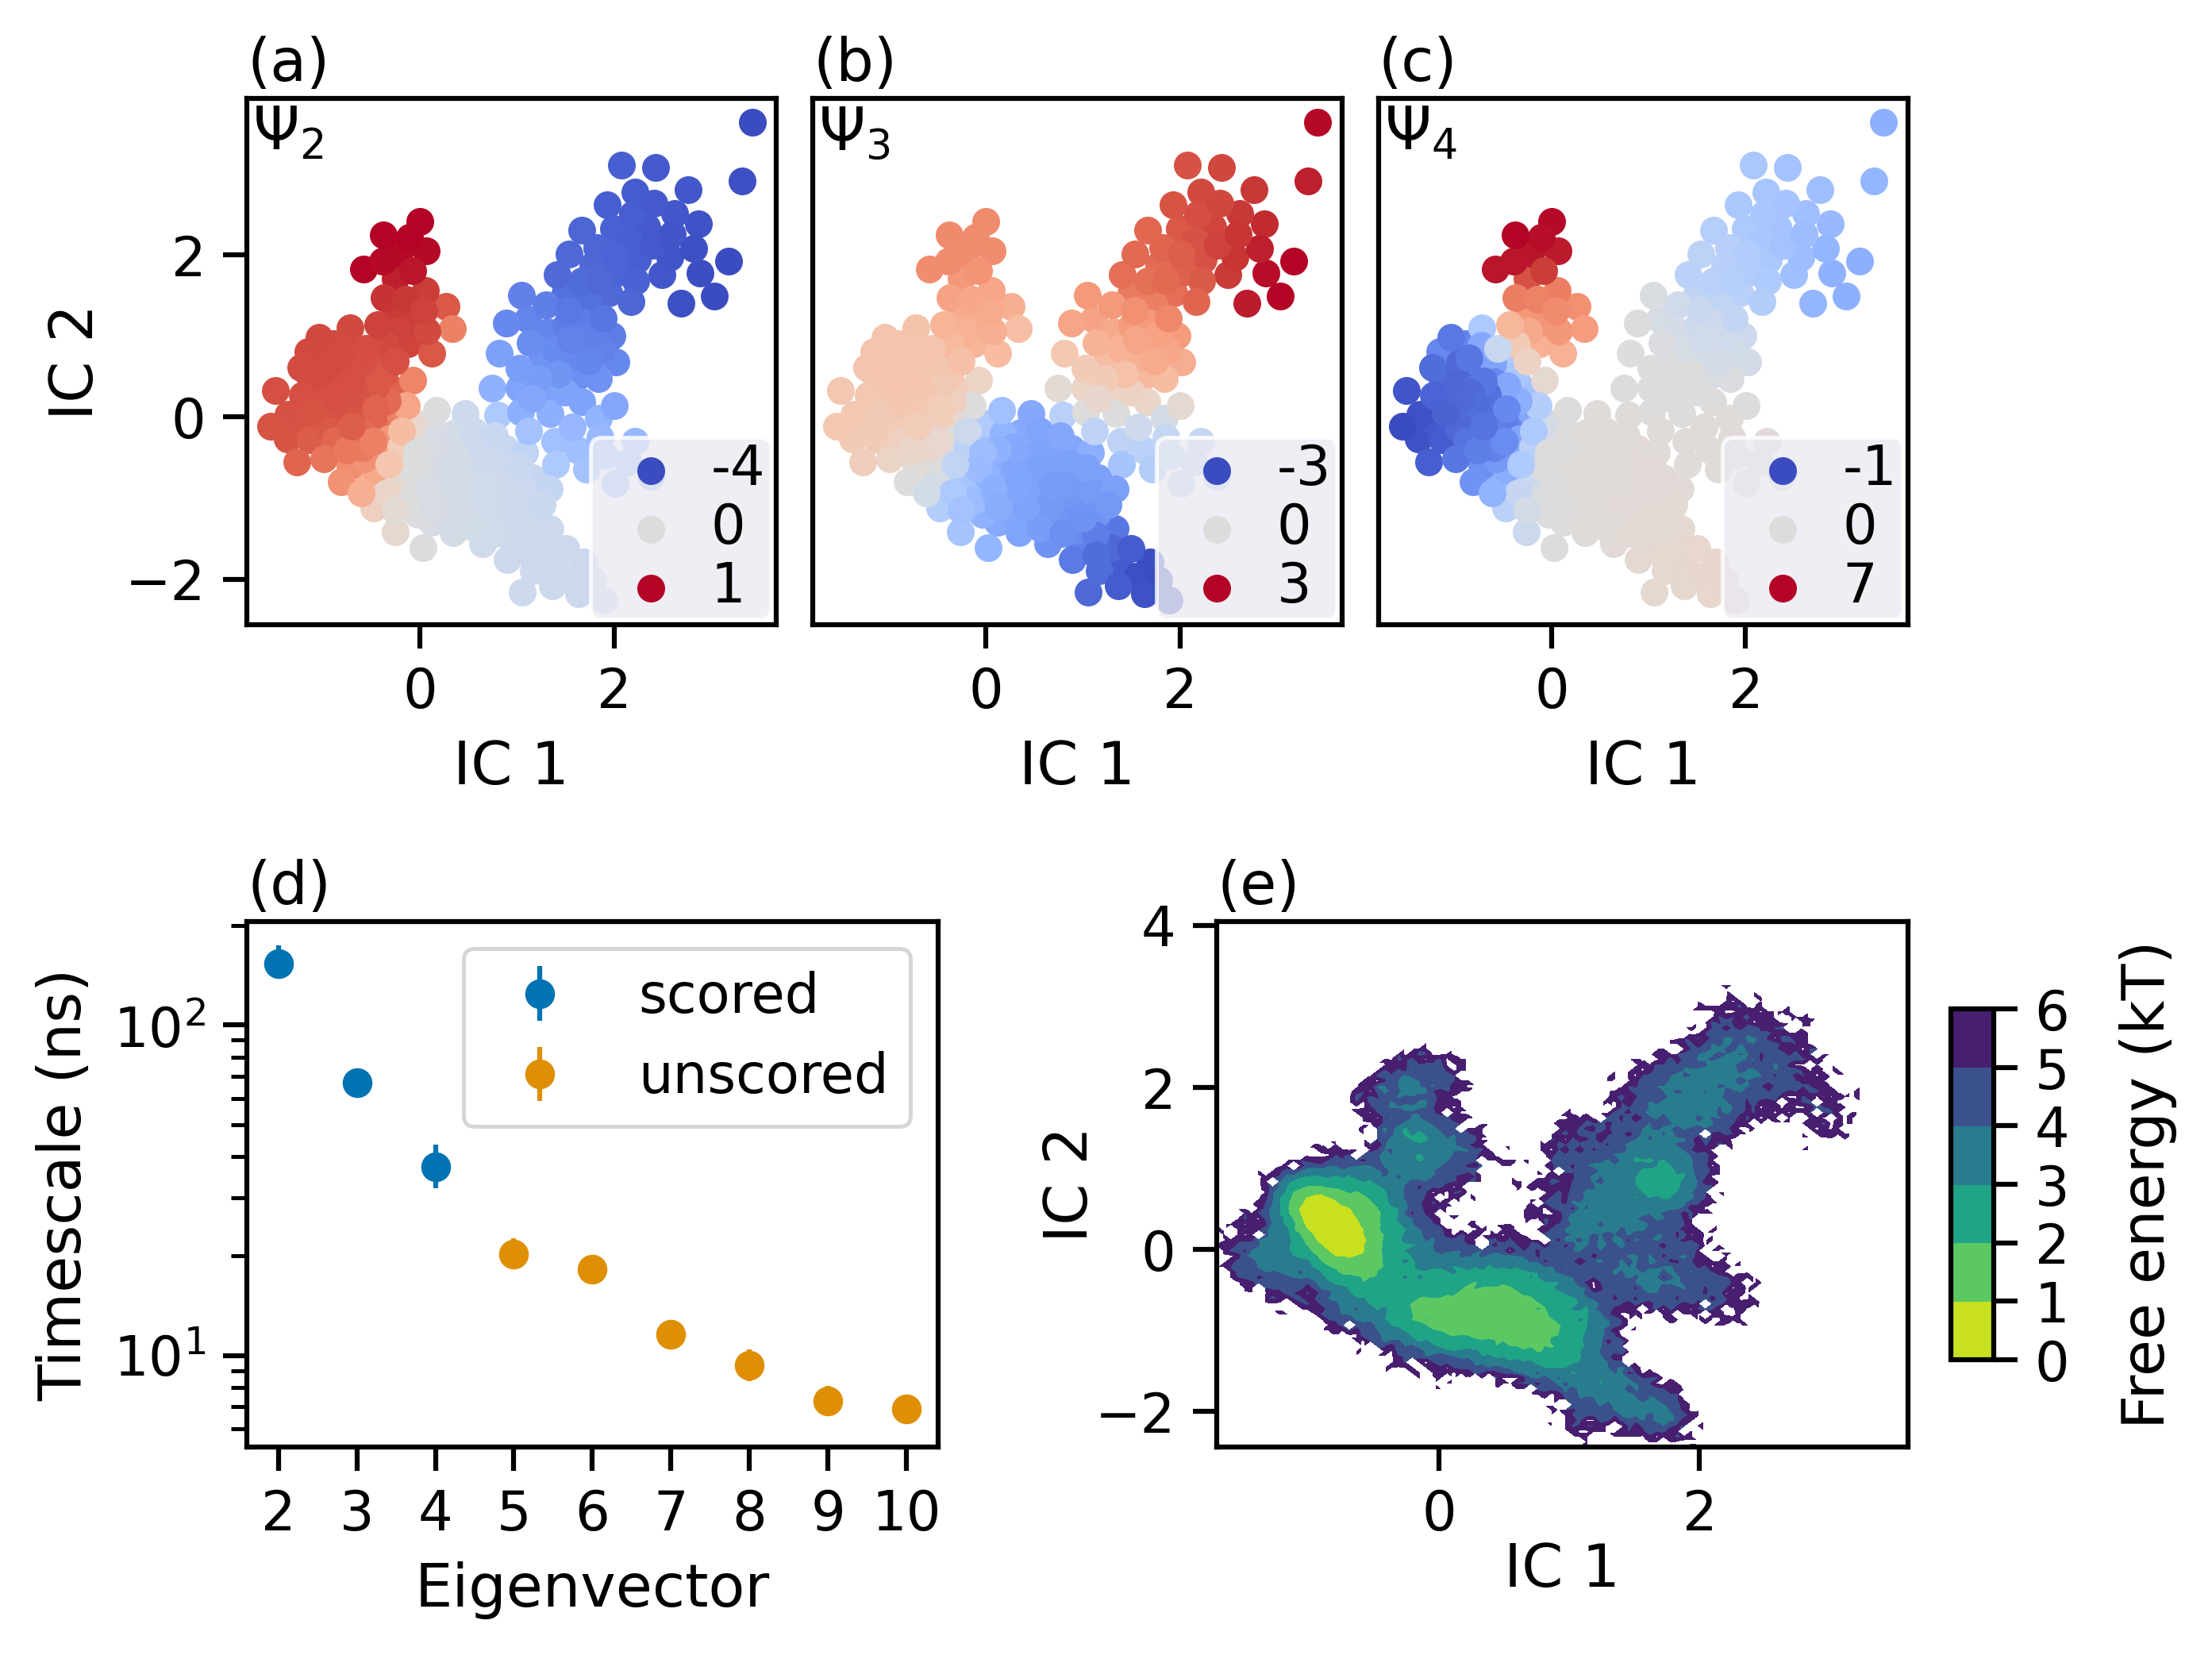
\includegraphics[width=0.8\textwidth]{chapters/msm_optimization/figures/aadh_msm_sens_3.png}
    \label{fig:aadh_msm_sens_3}
\end{figure}

\begin{figure}
    \centering
    \mycaption{Comparison of the first two TICA eigenvectors between base case, $\tau=\SI{10}{\nano\second}$ (blue) and sensitivity three $\tau=\SI{85}{\nano\second}$ (orange). The individual elements correspond to the weights associated with each of the $116$ dihedral features. Only the absolute values are shown. The elements were ordered according to the absolute value of the elements in the base case for each TICA component. The normalized overlap between the base case ($\mathbf{v}_{1}$) and sensitivity three ($\mathbf{v}_{2}$) is calculated as $\mathbf{v}_{1}\cdot\mathbf{v}_{2}/|\mathbf{v}_{1}||\mathbf{v}_{2}|$.}
    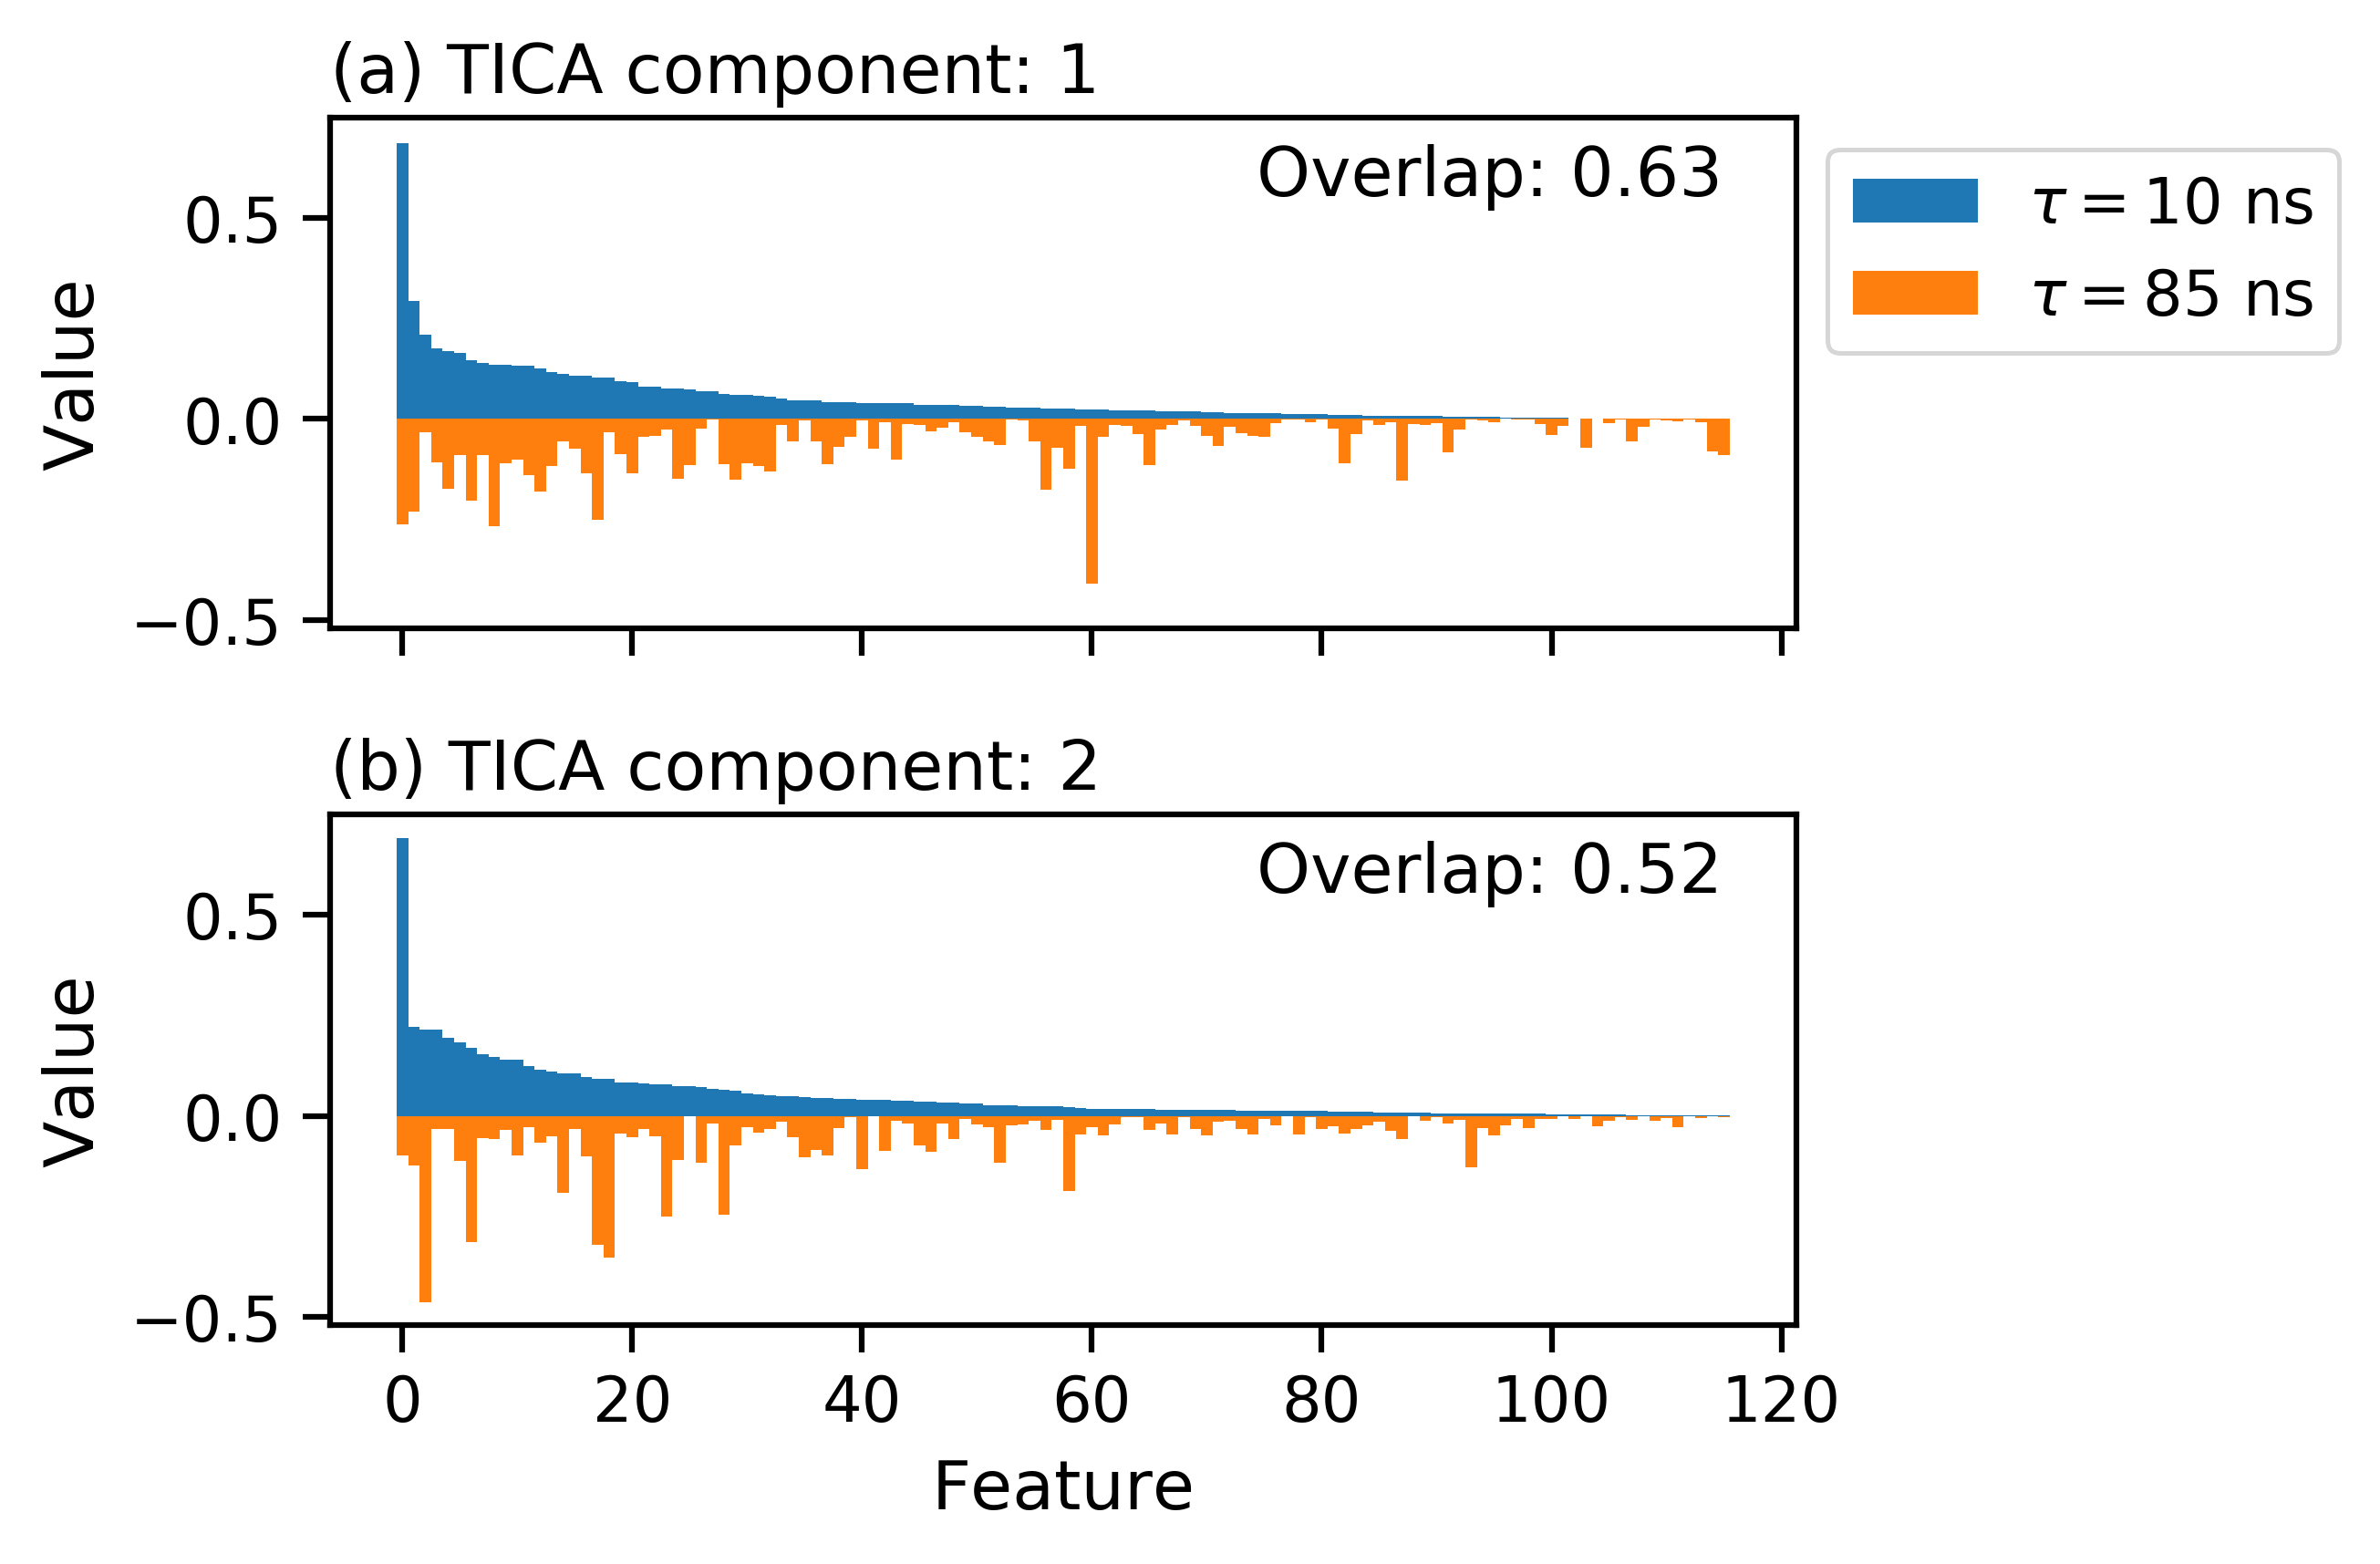
\includegraphics[width=0.8\textwidth]{chapters/msm_optimization/figures/aadh_msm_sens_3_tica.png}
    \label{fig:aadh_msm_sens_3_tica}
\end{figure}

Sensitivity 3, changed the value of $\tau$ to $\SI{85}{\nano\second}$ compared to the base case and is shown in figure \ref{fig:aadh_msm_sens_3}.   This value of $\tau$ was chosen because the response value at this point had the smallest  overlap with the incumbent (incumbent: $\mu=3.56 \pm 0.18$, sensitivity 3: $\mu=3.30 \pm 0.24$).  Here there is a distinct difference in the absolute values of the timescales and the free energy surface compared to the base case. To further delineate the difference between the two TICA representations, figure \ref{fig:aadh_msm_sens_3_tica} shows the difference between the first two TICA components. The  TICA components of the base case are shown in blue with the magnitude of the individual elements (corresponding to the $116$ dihedral features) ordered in decreasing value. The corresponding elements for this sensitivity are shown in orange with the sign flipped. The normalized overlap between the two TICA components of the base case and this sensitivity are $0.63$ and $0.56$  for the first and second TICA components respectively. This is due to the different weights attached to each dihedral feature. It is highly likely therefor that this represents a qualitatively and quantitatively different model. Where this change come in the response surface and and what the corresponding values of the response are will determine whether this an example of the Roshomon effect. 

\begin{table}
    \centering
    \mycaption{Mean implied timescales and $\SI{95}{\percent}$ credible intervals (in nanoseconds) of the relaxation processes 2 - 10 for the base case and three sensitivities.}

    \begin{tabular}{|l|l|l|l|l|}
    \hline
     &             Base Case &            Sensitivity 1 &         Sensitivity 2 &      Sensitivity 3 \\
    Process &                       &                          &                       &                    \\
    \hline\hline
    2       &  2,117 (1,033, 5,214) &  25,843 (15,913, 41,797) &  2,694 (1,352, 4,606) &   152 ( 138,  169) \\
    3       &     988 ( 479, 1,669) &     2,748 (1,510, 5,458) &      408 ( 312,  716) &    67 (  64,   71) \\
    4       &      231 ( 195,  276) &      1,101 ( 553, 2,256) &      304 ( 234,  397) &    36 (  31,   43) \\
    5       &      138 ( 129,  149) &         563 ( 497,  668) &      155 (  79,  252) &    20 (  19,   23) \\
    6       &       54 (  43,   73) &         482 ( 412,  566) &       80 (  52,  115) &    18 (  17,   20) \\
    7       &       38 (  33,   43) &         418 ( 327,  463) &       30 (  26,   38) &    12 (  11,   13) \\
    8       &       23 (  21,   26) &         228 ( 205,  249) &       25 (  22,   29) &     9 (   8,   10) \\
    9       &       21 (  18,   23) &         137 ( 115,  163) &       17 (  15,   18) &     7 (   7,    8) \\
    10      &       16 (  15,   19) &         105 (  99,  110) &       12 (  11,   15) &     7 (   6,    7) \\
    \hline
    \end{tabular}
    \label{tab:sens_ts}
\end{table}

{\huge This has been copied `as-is' from chapter \ref{chap:hmm}}
\section{HMMs}
\subsubsection{AADH}
The data for the AADH system comprise the MSMs and associated discrete trajectories of the base case and three sensitivities described in chapter \ref{chap:msm} section \ref{subsubsec:sensitivity_analysis}. The model specifications are tabulated here in table \ref{tab:aadh_final_msm_specs}. 

\begin{table}
    \centering
    \mycaption{Markov lag time and MSM hyper-parameters. These MSMs and the associated discrete trajectories form the data for the HMM coarse graining.}
    \begin{tabular}{|l|l|l|l|l|}
        \hline
        Parameter & Base case & Sensitivity 1 & Sensitivity 2 & Sensitivity 3 \\
        \hline\hline
        Markov lag time, $\tau(\textrm{MSM})$ & \SI{2}{\nano\second} &  \SI{20}{\nano\second}& \SI{2}{\nano\second}& \SI{2}{\nano\second} \\
        Feature, $\chi$ & $(\phi, \psi, \chi)$ & $(\phi, \psi, \chi)$ & $|\mathbf{r}_{1}-\mathbf{r}_2|$ & $(\phi, \psi, \chi)$ \\
        TICA lag time, $\tau$ & \SI{10}{\nano\second} & \SI{10}{\nano\second}&\SI{1}{\nano\second} &\SI{85}{\nano\second} \\
        TICA components, $m$ & $2$ & $2$ & $2$ & $2$ \\
        Cluster centres, $n$ & $310$ & $310$ & $110$ & $310$ \\
        \hline
    \end{tabular}
    \label{tab:aadh_final_msm_specs}
\end{table}



The state space of the HMMs was restricted to a reversibly connected set of  hidden states. This meant that for some stipulated values of $g$ the final model had $g^{\prime}<g$ hidden states. As this sub-setting was performed \emph{after} estimation, the degrees of freedom was still calculated using $g$. 

However, in the case of AADH the sub-setting of the state space meant re-scaling of the $\gamma_{i}(t)$ would necessary, negating the advantage of the first method, and so the second method was used. 

For AADH the information criteria were calculated for HMMs with $g = 2 - 20$ hidden states for each of the four different discretization specifications listed in table \ref{tab:aadh_final_msm_specs}.  The HMM with the smallest ICL was selected and estimated using a Bayesian hidden Markov model with two chains of  $1000$ burn-in steps and $1000$ sampling steps. The convergence of the transition matrix elements was checked using the Gelman-Rubin R-hat statistic. 

\section{Conformational landscape of AADH}


\section{Conclusions}
AADH is an important system for studying the effects of enzyme dynamics on catalysis due to the large kinetic isotope effect. Previous computational and experimental work determined the mechanism and estimated the free energy barriers using tryptamine as a substrate. The role of dynamics in explaining the temperature independent KIE in AADH is still unresolved. `Active dynamics` on the picosecond timescale have been suggested as facilitating tunneling, while  `passive dynamics', i.e. conformational dynamics, coupled with extensions of transition state theory, have also been suggested as explaining the behaviour of AADH's rate constant. To investigate the role of conformational dynamics in AADH, \SI{10}{\micro\second} of molecular dynamics simulations of the previously studied Schiff base intermediate were produced. A Markov lag time of $\tau=\SI{2}{\nano\second}$ and the number of dominant eigenvalues, $k=4$, were determined from an exploratory Markov state model. 

The validity of the simulations was limited however. An error in the preparation of the simulation resulted in the active site in the H chain missing an di-sulphide bond. The conformations of the H and D chains were radically different although surprisingly the H active site was more similar to the reactive conformations found in previous QM/MM studies. In addition, a number of unobserved residues were not modelled and there was correlation between each trajectory's initial configuration. Therefor a number of steps to improve this work: 

\begin{enumerate}
    \item Model the unobserved residues and fix the missing di-sulphide bonds in the crystal structure. 
    \item Solvate, energy minimize and equilibrate the initial structure. 
    \item From a long equilibration trajectory select $100$ configurations separated by \SI{10}{\nano\second} (the approximate Markov lag time from figure \ref{fig:its_d})), minimize and equilibrate these independently to create decorrelated initial configurations.
    \item  Use these initial configurations to seed $100$ production trajectories.
\end{enumerate}


